\documentclass[a4paper,12pt]{article}
\usepackage[utf8]{inputenc}
\usepackage[T2A]{fontenc}
\usepackage[russian]{babel}
\usepackage{amsmath}
\usepackage{colonequals}
\usepackage{amsfonts}
\usepackage{amssymb}
\usepackage[linesnumbered,boxed]{algorithm2e}
\usepackage{mathtools}
\usepackage{graphicx}
\usepackage{float}
\numberwithin{equation}{section}
\def\Xint#1{\mathchoice
	{\XXint\displaystyle\textstyle{#1}}%
	{\XXint\textstyle\scriptstyle{#1}}%
	{\XXint\scriptstyle\scriptscriptstyle{#1}}%
	{\XXint\scriptscriptstyle\scriptscriptstyle{#1}}%
	\!\int}
\def\XXint#1#2#3{{\setbox0=\hbox{$#1{#2#3}{\int}$}
		\vcenter{\hbox{$#2#3$}}\kern-.5\wd0}}
\def\ddashint{\Xint=}
\def\dashint{\Xint-}
%--- Number Sets ---
\newcommand{\N}{\mathbb N}
\newcommand{\R}{\mathbb R}
\newcommand{\Z}{\mathbb Z}
\newcommand{\Q}{\mathbb Q}

\newcommand{\defeq}{\colonequals}
\newcommand{\dd}{d}
\newcommand{\Ln}{\mathrm{Ln}\,}
\newcommand{\Arg}{\mathrm{Arg}\,}
\newcommand{\fext}{\varphi}
\newcommand{\fextp}{\tilde{\fext}}
\newcommand{\fextpp}{\bar{\fext}}
\newcommand{\ZZ}{\in \Z\setminus\{0\}}
\newcommand{\W}{W^H}

\newtheorem{Theorem}{Теорема}
\newtheorem{Lemma}{Лемма}
\newtheorem{Proposition}{Утверждение}
\newtheorem{Corollary}{Следствие}
\newtheorem{Remark}{Замечание}
\newtheorem{Definition}{Определение}
\newtheorem{Assumption}{Условие}
\newtheorem{problem}{Теорема}
\newtheorem{proof}{Доказательство}
\begin{document}
	
	\begin{titlepage}
		
		\newcommand{\HRule}{\rule{\linewidth}{0.5mm}} % Defines a new command for the horizontal lines, change thickness here
		
		\center % Center everything on the page
		
		%----------------------------------------------------------------------------------------
		%	HEADING SECTIONS
		%----------------------------------------------------------------------------------------
		
		\textsc{\LARGE Санкт-Петербургский государственный университет}\\[1.5cm] % Name of your university/college
		\textsc{\Large Кафедра теории вероятностей и математической статистики}\\[0.5cm] % Major heading such as course name
		\textsc{\large Курсовая работа}\\[0.5cm]
		%----------------------------------------------------------------------------------------
		%	TITLE SECTION
		%----------------------------------------------------------------------------------------
		\HRule \\[0.6cm]
		{ \Large \bfseries Cравнительный анализ алгоритмов моделирования дробного Броуновского движения}\\[0.4cm] % Title of your document
		\HRule \\[1.0cm]
		
		%----------------------------------------------------------------------------------------
		%	AUTHOR SECTION
		%----------------------------------------------------------------------------------------
		
		\begin{minipage}{0.4\textwidth}
			\begin{flushleft} \large
				\emph{Студент:}\\
				\textsc{Рагозин} Р.А. % Your name
			\end{flushleft}
		\end{minipage}
		~
		\begin{minipage}{0.4\textwidth}
			\begin{flushright} \large
				\emph{Научный руководитель:} \\
				\textsc{Русаков} О.В. % Supervisor's Name
			\end{flushright}
		\end{minipage}\\[2cm]
		
		%\Large \emph{Студент:}\\
		%Роман \textsc{Рагозин}\\[3cm] % %Your name
		
		
		%----------------------------------------------------------------------------------------
		%	LOGO SECTION
		%----------------------------------------------------------------------------------------
		
		
\includegraphics[width=100px]{Spbu-logo.png}\\[2cm] % Include a department/university logo - this will require the graphicx package
		
		
		%----------------------------------------------------------------------------------------
		%	DATE SECTION
		%----------------------------------------------------------------------------------------
		
		{\large 20 мая 2020 г.} % Date, change the \today to a set date if you want to be precise
		
		
		\vfill
		
		%----------------------------------------------------------------------------------------
		
	\end{titlepage}
	\newpage
	
	\section{Введение}
	Темой данной работы является моделирование дробного броуновского движения(дбд). Наиболее простое описание дбд следующее
	\begin{Definition}
		Дробное броуновское движение --- это центрированная случайная гауссовская функция $\W(t)$, $t\geq 0$ с нулевым начальным значением, которая имеет ковариационную функцию 
		\begin{align}
		\begin{split}\label{cov}
		K(s,t)\defeq cov(\W(s), \W(t)) = \frac{1}{2}\bigr(s^{2H}+t^{2H}-|s-t|^{2H}\bigr),
		\end{split}
		\end{align}
		где параметр $H \in (0,1]$ называется коэффициентом самоподобия или парметром Херста. 
	\end{Definition}
	Несложно заметить, что при $H = \frac{1}{2}$ данный процесс превращается в броуновское движение с нулевым начальным состоянием. Это следует из того, что $\min(s,t) = s+t - |s-t|$. Таким образом, функция ковариации и функция математического ожидания будут совпадать, а как известно, гауссовский процесс опредлеяется именно этими двумя функциями. 
	
	Также заметим, что при $H=1$ этот процесс имеет простой вид $\W(t) = tY$, где $Y$--- стандартная случайная величина. Значит этот процесс имеет линейные траектории, проходящие через точку $(1, \mathcal{N}(0,1))$. 
	
	Гауссовский процесс $\W(t)$ имеет непрерывную модификацию и обладает следующим свойством самоподобия 
	\begin{align}
	\begin{split}\label{selfsimilarity}
	\W(at) \overset{d}{=} a^H\W(t), \quad \forall a>0.
	\end{split}
	\end{align}
	Для начала докажем свойство самоподобия. Для начала заметим, что в левой и правой частях стоят гауссвские процессы. Значит осталось проверить, что совпадают их функции матожидания и функция ковариации. С первой функцией все очевидно, так как в обоих случаях это тождественный ноль. Покажем, что совпадают функции ковариации. 
	\begin{align}
	\begin{split}
	cov(\W(at), \W(as)) &= \frac{1}{2}\bigr((as)^{2H}+(at)^{2H}+ |as-at|^{2H} \bigr)  \\ &= a^{2H} cov(\W(s), \W(t))  \\ &=  cov(a^H\W(s), a^H\W(t)). 
	\end{split}
	\end{align}
	Таким образом, свойство самоподобия доказано. Теперь покажем, что процесс имеет непрерывную модификацию. Именно ее мы будем моделировать. Для доказательства непрерывности воспользуемся критерием Колмогорова, а именно подберем параметры $\varepsilon>0$, $K>0$ и $\beta>0$ такие что, для всех $s<t$ выполнено 
	\begin{align}
	\begin{split}\label{Kolmogorov}
	\mathbb{E}|\W(t)-\W(s)|^{\beta} \leq K |t-s|^{1+\varepsilon}.
	\end{split}
	\end{align} 
	Воспользуемся свойством самоподобия и получим
	\begin{align}
	\begin{split}
	\mathbb{E}|\W(t)-\W(s)|^{\beta} = \mathbb{E}\left|\left(\frac{t}{s}\right)^H\W(s)-\W(s)\right|^{\beta} = \frac{|t-s|^{H\beta}}{s^{H\beta}}\mathbb{E}|\W(s)|^{\beta}. 
	\end{split}
	\end{align}
	$\W(s)$--- гауссовская случайная величина с нулевым матожиданием и дисперсией $\mathbb{D}\W(s) = s^{2H}$. Тогда $\mathbb{E}|\W(s)|^{2n} = s^{2Hn} (2n-1)!!$, где $n \in \N$. Тогда возьмем в качестве $\beta = 2n$ и получим 
	\begin{align}
	\begin{split}
	\mathbb{E}|\W(t)-\W(s)|^{2n} = (2n-1)!! |t-s|^{2Hn}. 
	\end{split}
	\end{align}
	Достаточно взять $n$ настолько большим, что $2Hn>1$. Также из критерия Колмогорова будет с вероятностью 1 следовать гельдеровость порядка $\gamma<\frac{2Hn-1}{2n} = H-\frac{1}{2n}$. Так как это верно для любого $n \geq n_0$, то с вероятностью 1 будет гельдеровость порядка $\gamma<H$. 
	
	В данной работе будут рассмотрены два варианта моделирования дбд. Во второй главе будут приведены алгоритм и его теооретическое доказательство. Далее, в третьей главе будут приведены результаты работы алгоритма, а именно графики выборочных траекторий, и что-то еще. В четвертой главе будет произведен анализ работы алгоритмов и их сравнение.  
	\section{Алгоритмы}
	\subsection{Первый алгоритм}
	Первый вариант моделирования основан на дробном броуновском шуме(дбш), который задается последовательностью случайных велицин
	\begin{align}
	\begin{split}
	X_j = \W(j+1)-\W(j).
	\end{split}
	\end{align}
	Из определения дбд следует, что дбш это последовательность центрированных гауссовских случайных величин с ковариационной функцией 
	\begin{align}
	\begin{split}
	cov(X_n, X_{n+j}) &= \mathbb{E}(\W(n+1)-\W(n))(\W(n+j+1)-\W(n+j))\\ &= K(n+1, n+j+1) +K(n, n+j) \\ &- K(n+1, n+j)- K(n, n+j+1) \\ &= \frac{1}{2} \biggr[(n+1)^{2H} + (n+j+1)^{2H} \\ &-|n+1+j-n-1|^{2H} + n^{2H} + (n+j)^{2H} \\ &- |n+j-n|^{2H} - (n+1)^{2H} - (n+j)^{2H} \\ &+ |n+j-n-1|^{2H} n^{2H}-(n+j+1)^{2H} + |n+j+1-n|^{2H}  \biggr] \\ &= \frac{1}{2}\left(-|j|^{2H}-|j|^{2H}+|j-1|^{2H}+|j+1|^{2H} \right)  \\ &= \frac{1}{2}\left(|j-1|^{2H}- 2|j|^{2H}+|j+1|^{2H} \right).
	\end{split}
	\end{align}
	Представим алгоритм моделирования дбш. Пусть $\xi_k$, $k \in \Z$--- последовательность независимых стандартно распределеных случайных величин, $M>m$--- натуральные числа. Построим дбш следующим образом
	\begin{align}
	\begin{split}
	X_j = \frac{1}{\sqrt{m}C(H)}\sum_{n=1}^{Mm}K_H\left(\frac{n}{m}\right) \xi_{jm-n}, \quad j = 1,2,\ldots, 
	\end{split}
	\end{align}
	где функция $K_H(x)$ имеет вид
	\begin{align}
	\begin{split}
	K_H(x) = 
	\begin{cases}
	x^{H-1/2} - (x-1)^{H-1/2}, & x>1\\
	x^{H-1/2}, & 0<x\leq 1. 
	\end{cases}
	\end{split}
	\end{align}
	\begin{Theorem}
		$0<H<1$. Последовательность $X_j$, построенная выше, является приближением дробного броуновского шума. При $H=\frac{1}{2}$, последовательность $X_j$ в точости является дбш. 
	\end{Theorem}
	\textbf{Доказательство.} \quad Известно, что дробный броуновский шум имеет вид(см. \cite{Sam}, стр. 332)
	\begin{align}
	\begin{split}\label{integral}
	Y_j = \frac{1}{C(H)}\int_{-\infty}^{j+1} \biggr((j+1-x)_{+}^{H-1/2} - (j-x)_{+}^{H-1/2}  \biggr)M(\dd x),
	\end{split}
	\end{align}
	где 
	\begin{align}
	\begin{split}
	C(H) = \sqrt{\int_0^{\infty} \bigr((1+x)^{H-1/2}-x^{H-1/2} \bigr)^2 \dd x + \frac{1}{2H} },
	\end{split}
	\end{align}
	$M(dx)$--- случайная мера, такая что $M(A) \sim \mathcal{N}(0, \mu(A))$, где $\mu$--- мера Лебега. 
	
	Заметим, что выбор константы $C(H)$ обеспечивает единичную дисперсию для случайных величин $Y_j$, $j \in \N$. Действительно, 
	\begin{align}
	\begin{split}
	C^2(H)\mathbb{E}Y_j^2 &=  \mathbb{E}\left(\int_{-\infty}^{j+1} \bigr((j+1-x)_{+}^{H-1/2} - (j-x)_{+}^{H-1/2}  \bigr)M(\dd x)\right)^2 \\ &= \int_{-\infty}^{j+1} \bigr((j+1-x)_{+}^{H-1/2} - (j-x)_{+}^{H-1/2}  \bigr)^2 \dd x\\ &= \int_{-\infty}^{j} \bigr((j+1-x)^{H-1/2} - (j-x)^{H-1/2}  \bigr)^2 \dd x \\ &+ \int_{j}^{j+1} (j+1-x)^{2H-1} \dd x. 
	\end{split}
	\end{align} 
	В первом интеграле сделаем замену переменной $t = j-x$. А второй интеграл легко считается. Это будет $\frac{1}{2H}$. Тогда получим
	\begin{align}
	\begin{split}
	C^2(H)\mathbb{E}Y_j^2 = \int_{0}^{\infty} \bigr((t+1)^{H-1/2} - t^{H-1/2}  \bigr)^2 \dd t + \frac{1}{2H}. 
	\end{split}
	\end{align} 
	Поделим на $C^2(H)$ и получим, что $\mathbb{E}Y_j^2 = 1$. 
	
	Возьмем большое число $M \in \N$ и число $m \in \N$. Рассмотрим равномерное разбиение отрезка $[0, M]$, т.е. разбиение вида $\frac{i}{m}$, $i = 1, \ldots, mM$. Рассморим следующую случайную величину 
	\begin{align}
	\begin{split}
	Z(j,M) = \frac{1}{C(H)}\int_{j+1-M}^{j+1} \biggr((j+1-x)_{+}^{H-1/2} - (j-x)_{+}^{H-1/2}  \biggr)M(\dd x).
	\end{split}
	\end{align}  
	Воспользуемся свойством изометрии и получим
	\begin{align}
	\begin{split}
	\mathbb{E}(X_j-Z(j,M))^2 \\ &= \frac{1}{C^2(H)}\int_{-\infty}^{j+1-M}\biggr((j+1-x)_{+}^{H-1/2} - (j-x)_{+}^{H-1/2}  \biggr)^2 \\ \dd x \to 0, \, M \to \infty.  
	\end{split}
	\end{align}  
	Таким образом, есть сходимость $Z(j,M)$ к $Y_j$ при $M \to \infty$ в среднеквадратичном, а значит и по вероятности и по распределению. 
	
	Рассмотрим частичные суммы $Z(j,M)$. 
	\begin{align}
	\begin{split}
	Q(j, M, m) &= \frac{1}{C(H)} \sum_{k=1}^{mM} \biggr[(j+1-(j+1-k/m))_{+}^{H-1/2} \\ &- (j-(j+1-k/m))_{+}^{H-1/2}\biggr] M([\frac{k-1}{m}, \frac{k}{m}))\\ &= \frac{1}{C(H)} \sum_{k=1}^{mM} \biggr[\left(\frac{k}{m}\right)_{+}^{H-1/2} - \left(\frac{k}{m}-1\right)_{+}^{H-1/2}\biggr] M\left(\bigr[\frac{k-1}{m}, \frac{k}{m}\bigr)\right). 
	\end{split}
	\end{align}
	Заметим, что $(\frac{k}{m})_{+}^{H-1/2} - (\frac{k}{m}-1)_{+}^{H-1/2} = K_H(\frac{k}{m})$. Нам известно, что $M([\frac{k-1}{m}, \frac{k}{m}))$ имеет нормальное распредление с нулевым средним и дисперсией равной $1/m$. Тогда
	\begin{align}
	\begin{split}
	Q(j, M, m) = \frac{1}{\sqrt{m}C(H)} \sum_{k=1}^{mM} K_H(\frac{k}{m})\xi_{jm-n}, 
	\end{split}
	\end{align}
	где $\xi_{jm-n}$--- независимые, нормальные величины с нулевым матожиданием и единичной дисперсией. 
	
	Покажем, что при $H=1/2$ полученные случайные величины действительно будут дробным броуновским шумом. Для начала заметим, что $C(H)=1$. Так как $X_j$ являются линейными комбинациями гауссовских случайных величин, то и сами являются гауссовскими случайными величинами. Значит они определяются своими средними и автоковариационной функцией. Так как $\xi_k$--- стандартные гауссовские величины, то $\mathbb{E}X_j = 0$ для любого $l = 1,2,\ldots$. Осталось посчитать функцию автоковариации.
	\begin{align}
	\begin{split}
	m\mathbb{E}X_{j+l}X_j = \mathbb{E}\left(\sum_{n=1}^{Mm}K_H\left(\frac{n}{m}\right) \xi_{jm-n}\right)\left(\sum_{n=1}^{Mm}K_H\left(\frac{n}{m}\right) \xi_{(j+l)m-n}\right).
	\end{split}
	\end{align}
	Раскроем скобки и воспользуемся независимостью $\xi_k$. 
	\begin{align}
	\begin{split}
	m\mathbb{E}X_{j+l}X_j &= \sum_{p = lm+1}^{Mm}K_H\left(\frac{p-lm}{m}\right)K_H\left(\frac{p}{m}\right)\mathbb{E}\xi_{(j+l)m-p}^2 \\ &= \sum_{p = lm+1}^{Mm}K_H\left(\frac{p-lm}{m}\right)K_H\left(\frac{p}{m}\right).  
	\end{split}
	\end{align}
	Так как $H = 1/2$, то функция $K_H(x)$ имеет простой вид 
	\begin{align}
	\begin{split}
	K_H(x) = 
	\begin{cases}
	0, & x>1\\
	1, & 0<x\leq 1. 
	\end{cases}
	\end{split}
	\end{align}
	Для начала рассмотрим случай когда $l\geq 1$. Тогда $K_H\left(\frac{p}{m}\right) = 0$ для любого $p \geq lm+1$. Значит при $l \geq 1$ верно, что $\mathbb{E}X_jX_{j+l} = 0$, что и будет для шумов броуновского движения. 
	
	Рассмотрим случай, когда $l = 0$, т.е. мы должны вычислить $\mathbb{E}X_j^2$. Для шумов броуновского движения известно, что $\mathbb{E}X_j^2 = 1$ для всех $j$. В нашей задаче мы получаем 
	\begin{align}
	\begin{split}
	m\mathbb{E}X_j^2 =  \sum_{n=1}^{Mm}K_H^2\left(\frac{n}{m}\right) = \sum_{n=1}^{m}K_H^2\left(\frac{n}{m}\right) = \sum_{n=1}^{m}1 = m. 
	\end{split}
	\end{align} 
	$\Box$
	
	\textbf{Реализация алгоритма} \quad Производится равномерное разбиение интервала на $T$ частей. Каждому узлу разбиения, начиная с первого, приписывается нормированное значение дбд. Нормирующие коэффициенты дбш легко вычисляются в соответствие с длиной шага разбиения путем применения соотношения самоподобия $\eqref{selfsimilarity}$. Далее, для получения непрерывной траетории дбд, значения в узлах линейно экстраполируются. 
	
	В алгоритме параметр $M$ отвечает за "память" процесса, а парметр $m$ --- за "настоящее" процесса. Рекомендуется, чтобы $M$ было больше $m$ в 10-15 раз, и $M$ примерно ровнялось $T$. Вполне удовлетворительные результаты получаются уже при $M=T=500$, $m=30$.
	\begin{Remark}
		Данный алгоритм требует генерирования $m(T+M-1)$ независимых одинаково распределенных случайных величин. Для реализации броуновского движения требуется лишь $T$ н.о.р.с.в, а для дбд с $H=1$ всего одной. Таким образом, при $H=1/2$ или $H=1$ лучше использовать другие алгоритмы. 
	\end{Remark}
	\subsection{Второй алгоритм}
	Пусть $(\Omega, \mathfrak{F}, \mathbb{P})$--- вероятностное пространство, на котором заданы все случайные величины. Пусть $\Pi_1(s)$, $s \geq 0$--- стационарный пуассоновский процесс с единичной интенсивностью, $(\xi) = \xi_0, \xi_1, \ldots$--- последовательность случайных величин. Будем называть такую последовательность образующей. Пусть $\lambda = \lambda(\omega)$, $\omega \in \Omega$--- неотрицательная (п.н.) случайная величина с функцией распределения $F_{\lambda}(x)$, $x\geq 0$. Будем считать, что $\Pi_1(s)$, $(\xi)$ и $\lambda$ взаимно незавиимы. 
	\begin{Definition}
		Пуассоновский субординатор со случайной интенсивностью $\lambda(\omega)$ для последовательности $(\xi)$, или дважды стохастический псевдо пуассоновский процесс со случайной интенсивностью $\lambda(\omega)$ --- это случайный процесс $\psi(s)$, $s \geq 0$, определенный равенством 
		\begin{align}
		\begin{split}\label{subor}
		\psi(s) = \psi_{\lambda}(s) = \psi_{\lambda(\omega)}(s) = \xi_{\Pi_{\lambda(\omega)}(s)}, 
		\end{split}
		\end{align} 
		где 
		\begin{align}
		\begin{split}\label{poisson}
		\Pi_{\lambda(\omega)}(s) = \Pi_1(\lambda(\omega)s) = \Pi_1(\lambda s). 
		\end{split}
		\end{align}
	\end{Definition}
	Процесс $\psi$, определенный в \eqref{subor} будем называть PSI(Poisson Stochastic Index) процессом. 
	
	Приведем несколько утверждений, доказательство которых описано в статье(см. \cite{Rusakov}). 
	\begin{Lemma}
		Пусть $(\xi)$--- последовательность независимых одинаково распределенных случайных величин. Тогда субординатор $\psi_{\lambda(\omega)}(t)$---  стационарный процесс в узком смысле. Значит он может быть продолжен на всю вещественную прямую. 
	\end{Lemma}
	\begin{Lemma}
		Пусть $\mathbb{D}\xi_0 = 1$. Тогда автоковариационная функция совпадает с преобразованием Лапласа $L_{\lambda}(t)$, $t \geq 0$ функции распределения $\lambda(\omega)$, а именно 
		\begin{align}
		\begin{split}
		cov(\psi_{\lambda}(v), \psi_{\lambda}(v+s)) = \int_0^{\infty} \exp(-st)\dd F_{\lambda}(t) =: L_{\lambda}(s). 
		\end{split}
		\end{align}   
	\end{Lemma}
	\begin{Lemma}
		Введем следующий интеграл 
		\begin{align}
		\begin{split}\label{integralPSI}
		\Psi(t) = \int_0^t \xi_{\Pi_{\lambda}(u)} \dd u. 
		\end{split}
		\end{align}
		Тогда ковариация проинтегрированного PSI процесса вычисляется следующим образом 
		\begin{align}
		\begin{split}
		cov(\Psi(s), \Psi(t)) = \sigma_0^2 \int_0^t\int_0^s L_{\lambda}(|x-y|)\dd x \dd y, 
		\end{split}
		\end{align}
		где $s, t \geq 0$, $\sigma_0^2 = \mathbb{D}\xi_0$, $\sigma_0>0$.  
	\end{Lemma}
	\begin{Definition}
		Случайная величина $X$ имеет гамма распределение с параметром формы $\varkappa$ и парметром масштаба $\theta$, если 
		\begin{align}
		\begin{split}
		\frac{\dd}{\dd x}\mathbb{P}(X<x) = \frac{x^{\varkappa-1}}{\theta^{\varkappa}\Gamma(\varkappa)} \exp\left(-\frac{x}{\theta}\right)\mathbb{I}_{x>0}. 
		\end{split}
		\end{align}
		Будем обозначать это так: $X \sim \Gamma(\varkappa, \theta)$. 
	\end{Definition}
	\begin{Proposition}
		Пусть $(\xi)$--- последовательность независимых одинаково распределенных случайные величин с $\mathbb{E}\xi_0 = \mu$, $\mu \in \R$ и с $\mathbb{D}\xi_0 = \sigma_0^2$, $\sigma_0>0$. Пусть $\Pi_1(t)$--- стационарный пуассоновский процесс с единичной интенсивностью, $t \geq 0$. Пусть $\lambda(\omega) \sim \Gamma(\varkappa, \theta)$. 
		
		Предположим, что $(\xi)$, $\Pi_1(t)$ и $\lambda$ взаимно независимы. Определим процесс $\psi_{\lambda}(t)$ по формуле \eqref{subor} и процесс $\Psi(t)$, определенный по формуле \eqref{integralPSI}. Тогда 
		
		1) Если $\varkappa \ne 1$ и $\varkappa \ne 2$, то 
		\begin{align}
		\begin{split}
		cov(\Psi_{\lambda}(t), \Psi_{\lambda}(s)) &= \frac{\sigma_0^2}{(1-\varkappa)(2-\varkappa)\theta^{\varkappa}}\times \biggr( (t+1/\theta)^{2-\varkappa} \\ &+ (s+1/\theta)^{2-\varkappa} -(|t-s| +  1/\theta)^{2-\varkappa}\\ &-2(2-\varkappa)\min(s,t )(1/\theta)^{1-\varkappa}-(1/\theta)^{2-\varkappa}\biggr);
		\end{split}
		\end{align}
		
		2) Если $\varkappa = 2$, то 
		\begin{align}
		\begin{split}
		cov(\Psi_{\lambda}(t), \Psi_{\lambda}(s)) &= \frac{\sigma_0^2}{\theta^2} \biggr( \ln(|t-s|+1/\theta) \\ &- \ln(t+1/\theta)- \ln(s+1/\theta)+2\theta\min(s,t)-\ln \theta \biggr);
		\end{split}
		\end{align}
		
		3) Если $\varkappa = 1$, то 
		\begin{align}
		\begin{split}
		cov(\Psi_{\lambda}(t), \Psi_{\lambda}(s)) &= \frac{\sigma_0^2}{\theta} \biggr( -(|t-s|+1/\theta)\ln(|t-s|+1/\theta) \\ &+ (t+1/\theta)\ln(t+1/\theta)+ (s+1/\theta)\ln(s+1/\theta) \\ &+ 2\ln \theta \min(s,t) +\ln \theta/\theta -2\min(s,t)  \biggr);
		\end{split}
		\end{align}
	\end{Proposition}
	\begin{Theorem}
		Пусть $(\xi)$--- последовательность независимых одинаково распределенных случайные величин с $\mathbb{E}\xi_0 = 0$ и с 
		\begin{align}
		\begin{split}
		\mathbb{D}\xi_0 = \mathbb{D}\xi_0(\varkappa, \theta) = \frac{1}{2}(2-\varkappa)(1-\varkappa)\theta^{\varkappa},
		\end{split}
		\end{align}
		где $0<\varkappa<1$, $\theta>0$--- фиксированные числа. 
		
		Пусть $\Pi_1(t)$--- стационарный пуассоновский процесс с единичной интенсивностью, $t \geq 0$. Пусть $\lambda(\omega) \sim \Gamma(\varkappa, \theta)$. 
		
		Предположим, что $(\xi)$, $\Pi_1(t)$ и $\lambda$ взаимно независимы. Определим процесс $\psi_{\lambda}(t)$ по формуле \eqref{subor} и процесс $\Psi_{\varkappa, \theta}(t)$, определенный по формуле \eqref{integralPSI}. 
		
		Тогда ковариационная функция процесса $\Psi(t)$ сходится к ковариационной функции дробного броуновского движения равномерно на любом компакте в $[0,T]$ при стремлении парметра $\theta$ к бесконечности. А именно, 
		\begin{align}
		\begin{split}
		cov(\Psi_{\varkappa, \theta}(t), \Psi_{\varkappa, \theta}(s)) \to \frac{1}{2}(s^{2H} + t^{2H}-|s-t|^{2H}), \quad \theta \to \infty,
		\end{split}
		\end{align} 
		где $H = 1-\varkappa/2 \in (1/2, 1)$--- параметр Херста. 
	\end{Theorem}
	Пусть $\{\Psi_{\varkappa, \theta}(t)^{[j]}\}$, $j \in \N$--- независимые копии процесса $\{\Psi_{\varkappa, \theta}(t)$, $t \geq 0$. 
	\begin{Theorem}
		\begin{align}
		\begin{split}
		\frac{1}{\sqrt{N}}\sum_{j=1}^{N}\Psi_{\varkappa, \theta}(t)^{[j]} \Rightarrow W_{\varkappa, \theta}(t), \, t\geq 0, 
		\end{split}
		\end{align}
		где под знаком $\Rightarrow$ понимается слабая сходимость распределений, а $W_{\varkappa, \theta}(t)$--- начинающийся в нуле, центрированный гауссовский процесс со стационарными приращениями.  
		
		При этом, ковариационная функция процесса $W_{\varkappa, 
			\theta}(t)$ имеет вид
		\begin{align}
		\begin{split}
		cov(W_{\varkappa, 
			\theta}(t), W_{\varkappa, 
			\theta}(s)) &= \frac{1}{2}\biggr( (t+1/\theta)^{2-\varkappa} + (s+1/\theta)^{2-\varkappa}-(|t-s| +  1/\theta)^{2-\varkappa}\\&-2(2-\varkappa)\min(s,t )(1/\theta)^{1-\varkappa}-(1/\theta)^{2-\varkappa}\biggr). 
		\end{split}
		\end{align}
	\end{Theorem} 
	\begin{Corollary}
		Ковариационная функция процесса $W_{\varkappa, 
			\theta}(t)$ сходится к ковариационной функции дробного броуновского движения равномерно на любом компакте в $[0,T]$ при стремлении парметра $\theta$ к бесконечности. А именно, 
		\begin{align}
		\begin{split}
		cov(W_{\varkappa, 
			\theta}(t), W_{\varkappa, 
			\theta}(s)) \to \frac{1}{2}(s^{2H} + t^{2H}-|s-t|^{2H}), \quad \theta \to \infty,
		\end{split}
		\end{align} 
		где $H = 1-\varkappa/2 \in (1/2, 1)$--- параметр Херста. 
	\end{Corollary}
	\begin{Theorem}
		Пусть $\varkappa = 1$ и $(\xi)$--- н.о.р.с.в. с дисперсией $\mathbb{D}\xi_0 = \mathbb{D}\xi_0(\theta) = \frac{\theta}{2\ln \theta}$, $\theta>1$ или $\varkappa >1$ и $\mathbb{D}\xi_0 = \mathbb{D}\xi_0(\varkappa, \theta) = \frac{(\varkappa-1)\theta}{2}$, $\theta>0$. Тогда ковариация проинтегрированного PSI процесса сходится к ковариации броуновского движения при $\theta \to \infty$:
		\begin{align}
		\begin{split}
		cov(\Psi_{\varkappa, \theta}(t), \Psi_{\varkappa, \theta}(s)) \to \min(s,t).
		\end{split}
		\end{align}
		При этом, сходимость равномерна на каждом компакте в $[0,T]$. 
	\end{Theorem}
	\textbf{Реализация алгоритма} \quad Сначала зафиксируем параметр Херста $H \in (1/2, 1)$. Смоделируем с.в. $\lambda$, которая имеет гамма распределение с параметром формы $\varkappa = 2-2H$ и парметром масштаба $\theta \gg 1$(Например, можно брать $\theta = 100, 1000, 10000$ и т.д.). Выберем число $T>0$(в данной работе было взято $T = 1$ для всех экспериментов). Затем смоделируем пуассоновский процесс, интенсивности $\lambda$ на отрезке $[0,T]$. Далее моделируем неоходимое число с.в. $\xi_k$, $k =0, \ldots, L$. Отцентрируем и отнормируем с.в. $\xi_k$, $k = 0, \ldots, L$ так, чтобы они удовлетворяли условиям теоремы~2. На последнем шаге смоделируем PSI процесс и посчитаем от него интеграл. 
	\begin{Remark}
		Данный алгоритм требует реализации гамма распределенной случайной величины с нецелым параматером. Данная задача не имеет простого решения, но при этом число операций не зависит от $\theta$. Затем надо моделировать $L$ случайных величин. $L$--- случайное число. Оценим его математическим ожиданием. Будем считать, что $L$ эквивалентно $T\varkappa \theta$. Таким образом, требуется генерирование порядка $\varkappa\theta$ случайных величин. Это дает преимущество, если $H$ близко к 1. 
	\end{Remark}
	\subsection{Моделирование распределений}
	\subsubsection{Нормальное распределение}
	
	Рассмотрим $\mathbf{z} = (\xi, \eta)$ стандартный гауссовский вектор, т.е. $p_{\mathbf{z}}(x,y) = \frac{1}{2 \pi} \exp \left(-\frac{x^2 + y^2}{2} \right)$. Если мы перейдём к полярным координатам $x=r \sin \varphi$, $y= r \cos \varphi$, то:
	
	\begin{equation}
		p_{\mathbf{z}}(r , \phi) = \frac{r}{2 \pi} \exp \left(-\frac{r^2}{2} \right).
	\end{equation}
	
	Таким образом, $\Arg (\xi+i \eta) $ равномерно распределён на $[0, 2 \pi)$, а $r = |\xi+i \eta|$ имеет плотность $p_{|\mathbf{z}|}(r) =  r\exp \left(-\frac{r^2}{2} \right)$ и  $F_{|\mathbf{z}|}(t) = 1-\exp \left(-\frac{t^2}{2} \right)$. . Но по формуле обращения $\xi = \sqrt{-2 \ln \alpha}$, где $\alpha$ имеет равномерное распределение на $[0,1]$. Таким образом, будем моделировать нормальную величину следующим образом:
	
	$
	\begin{array}{l}
	\xi = \sqrt{-2 \ln \alpha_1} \cos \, 2 \pi \alpha_2;\\
	\eta = \sqrt{-2 \ln \alpha_1} \sin \, 2 \pi \alpha_2.\\
	\end{array}
	$
	
	где $\alpha_1, \alpha_2$ независимы и равномерно распределены на $[0,1]$.
	
	Алгоритм ниже иллюстрирует принцип работы $\texttt{Norm}$
	
	\begin{algorithm}[H]
		\SetAlgoLined %% Это соединяет линиями логические части
		%% алгоритма типа if-then-else
		
		\KwData{ Генератор равномерного на $[0,1]$ распределения \texttt{RANDOM()} с независимыми вызовами}
		
		\KwResult{ Вектор $( x_1, x_2 )$ имеющий стандартное нормальное распределение} %% результат работы программы
		
		$\alpha_1$ \texttt{ = RANDOM()}
		
		$\alpha_2$ \texttt{ = RANDOM()}
		
		$x_1$  = $\sqrt{-2 \ln \alpha_1} \cos \, 2 \pi \alpha_2$
		
		$x_2$  = $\sqrt{-2 \ln \alpha_1} \sin \, 2 \pi \alpha_2$
		
		\caption{Схема работы \texttt{Norm}}
		% \label{alg:generalGP}
	\end{algorithm}
	\subsubsection{Гамма-распределение}
	
	Также нам потребуется смоделировать с.в. $\xi$, имеющую гамма-распределение. В данном случае нужно моделировать гамма-распределение с параметром формы $\varkappa =2-2H$, где $H \in (1/2,1)$. Значит $\varkappa \in (0,1)$. Также вспомним, что если $\lambda \sim \Gamma(\varkappa, 1)$, то $\theta \lambda \sim \Gamma(\varkappa, \theta)$. Значит достаточно реализовать алгоритм для гамма-распределения с парметром масштаба $\theta = 1$.     
	
	Докажем одно полезное утверждение. Оно позволяет сократить число генерируемых с.в. в случае когда $H = 3/4$. 
	\begin{Proposition}\label{3}
		Пусть $N$  имеет стандартное нормальное распределение, тогда  $\frac{1}{2}N^2 \sim \Gamma(1/2, 1)$
	\end{Proposition}
	\begin{proof}
		Пусть $x\in (0;+\infty)$
		\begin{align}
		\begin{split}
		\mathbb{P}(\frac{1}{2}N^2<x) &= \mathbb{P}(N^2<2x) = \mathbb{P}(N \in (-\sqrt{2x},\sqrt{2x}))\\ &=\frac{1}{\sqrt{2\pi}} \int_{-\sqrt{2x}}^{\sqrt{2x}}e^{-\frac{t^2}{2}}dt = \frac{2}{\sqrt{2\pi}}\int_{0}^{\sqrt{2x}}e^{-\frac{t^2}{2}}dt. 
		\end{split}
		\end{align} 
		Найдем плотность данной случайной величины
		\begin{align}
		\begin{split}
		p(x) = \frac{d}{dx}  \frac{2}{\sqrt{2\pi}}\int_{0}^{\sqrt{2x}}e^{-\frac{t^2}{2}}dt = \frac{2}{\sqrt{2\pi}}e^{-\frac{2x}{2}}\frac{1}{\sqrt{2x}} = \frac{1}{\sqrt{\pi}}x^{1-\frac{1}{2}}e^{-x}.
		\end{split}
		\end{align}
		Таким образом,  $\frac{1}{2}N^2 \sim $ Gamma($\frac{1}{2},$ 1).
	\end{proof} 
	
	Для построения гамма-распределения воспользуемся улучшенным алгоритмом Вадувы. Обоснование алгоритма приведено в книге $\cite{Devroye}$, стр. 415.  
	
	\begin{algorithm}[H]
		\SetAlgoLined %% Это соединяет линиями логические части
		%% алгоритма типа if-then-else
		
		\KwData{ Число $\varkappa \in (0,1)$, генератор равномерного на $[0,1]$ распределения \texttt{RANDOM()} с независимыми вызовами}
		
		\KwResult{ $X$ имеющая распределение $\Gamma(\varkappa, 1)$ } %% результат работы программы
		\If{$\varkappa = \frac{1}{2}$}{
			
			N = Norm()
			
			$X = \frac{1}{2}N^2$
			
		}
		
		\If{$\varkappa \ne 1/2$}{
			$c = \frac{1}{\varkappa}$
			
			$d = \varkappa^{\frac{\varkappa}{1-\varkappa}}(1-\varkappa)$
			
			Accept = False
			
			\While{ Not Accept}{
				Z = $-\ln(\texttt{RANDOM()})$	
				
				E = $-\ln(\texttt{RANDOM()})$
				
				$X = Z^{c}$
				
				Accept = [Z+E$\leq$ d+$X$]
			}
			
		}
		\caption{Схема работы $
			\Gamma(\varkappa,1)$}
		% \label{alg:generalGP}
	\end{algorithm}
	\subsubsection{Моделирование пуассоновского процесса с постоянной интенсивностью $\lambda$}
	Рассмотрим пуассоновский процесс $\Pi_{\lambda}(t)$, где $t \geq 0$. 
	
	Обозначим через $\tau_k$ длину участка, на котором $\Pi_{\lambda}(t)$ равен $k$, $k = 0,1,2,\ldots$. Известно, что $\tau_k$ имеют экспоненциальное распределение с плотностью $\lambda e^{-\lambda t}\mathbb{I}_{t>0}$, $t\geq 0$. Таким образом, достаточно уметь моделировать экспоненциальные случайные величины.
	
	Пусть случайная величина $\xi$ имеет экспоненциальное распределение, т.е. $\mathbb{P}(\xi < x) = 1-e^{\lambda x}$, $x \geq 0$. Тогда по лемме Смирнова $1 - e^{\lambda \xi}$ имеет равномерное на $[0,1]$ распределение. Таким образом, $\xi = -\frac{\log(1-\alpha)}{\lambda}$, где $\alpha$ имеет равномерное на $[0,1]$ распределение, но тогда и $1-\alpha$ имеет равномерное на $[0,1]$ распределение, а это значит, что $\xi = -\frac{\log \alpha}{\lambda}$. 
	
	\begin{algorithm}[H]
		\SetAlgoLined %% Это соединяет линиями логические части
		%% алгоритма типа if-then-else
		
		\KwData{ Генератор равномерного на $[0,1]$ распределения \texttt{RANDOM()} с независимыми вызовами, интенсивность $\lambda$, число $T>0$}
		
		\KwResult{ Массив Array точек роста пуассоновского процесса $\Pi_{\lambda}(t)$} %% результат работы программы
		
		$\alpha$ \texttt{ = RANDOM()}
		
		$\sigma = -\frac{\log \alpha}{\lambda}$
		
		Array <- $\sigma$
		
		\texttt{while} $(\sigma < T)$:
		
		$\alpha_1$ \texttt{ = RANDOM()}
		
		$\sigma = \sigma - \log \alpha_1/\lambda$
		
		Array <- $\sigma$
		
		\texttt{end}
		
		\caption{Схема построения точек роста пуассоновского процесса на [0,T]}
		% \label{alg:generalGP}
	\end{algorithm}
	\section{Результаты моделирования}
	\subsection{Первый алгоритм}
	Ниже представлены графики 100 траекторий дробного броуновского движения, смоделированных первым алгоритмом с параметрами: $T=M=250$, $m=15$:
	\begin{figure}[H]
		\minipage{0.49\textwidth}
		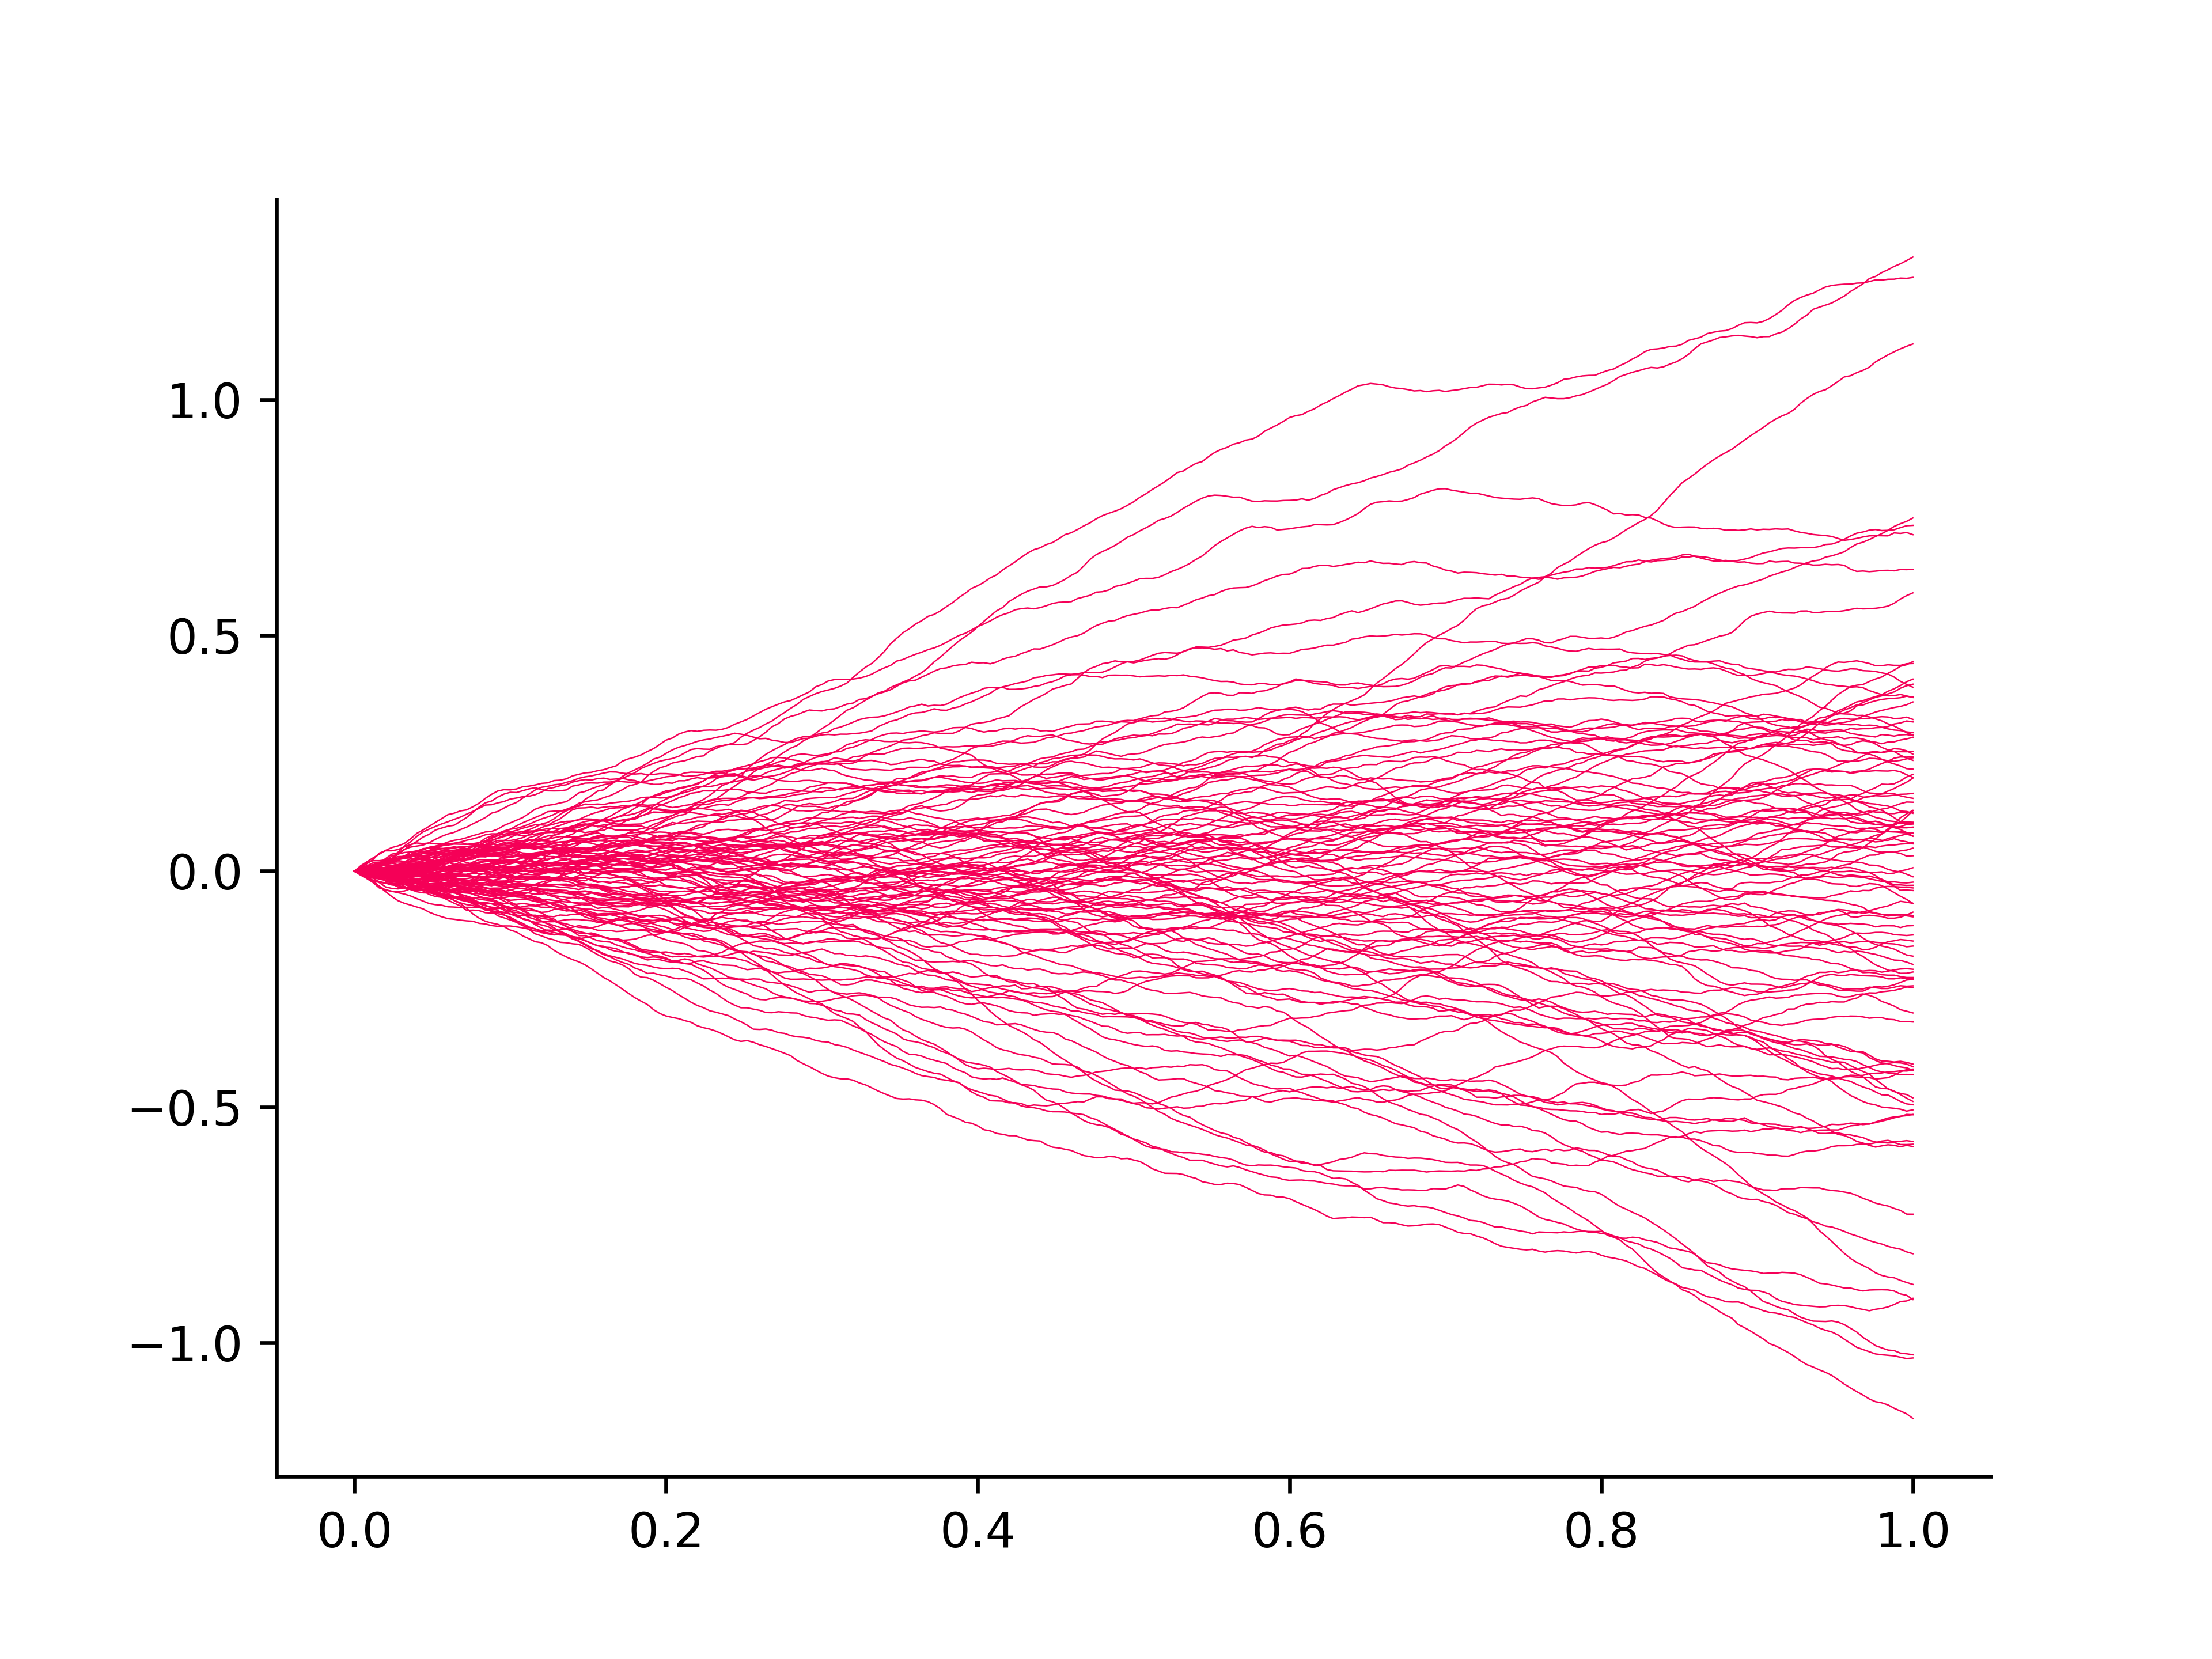
\includegraphics[scale=0.4]{image-1-95.png}
		\caption{H=0.95}
		\endminipage\hfill
		\minipage{0.49\textwidth}
		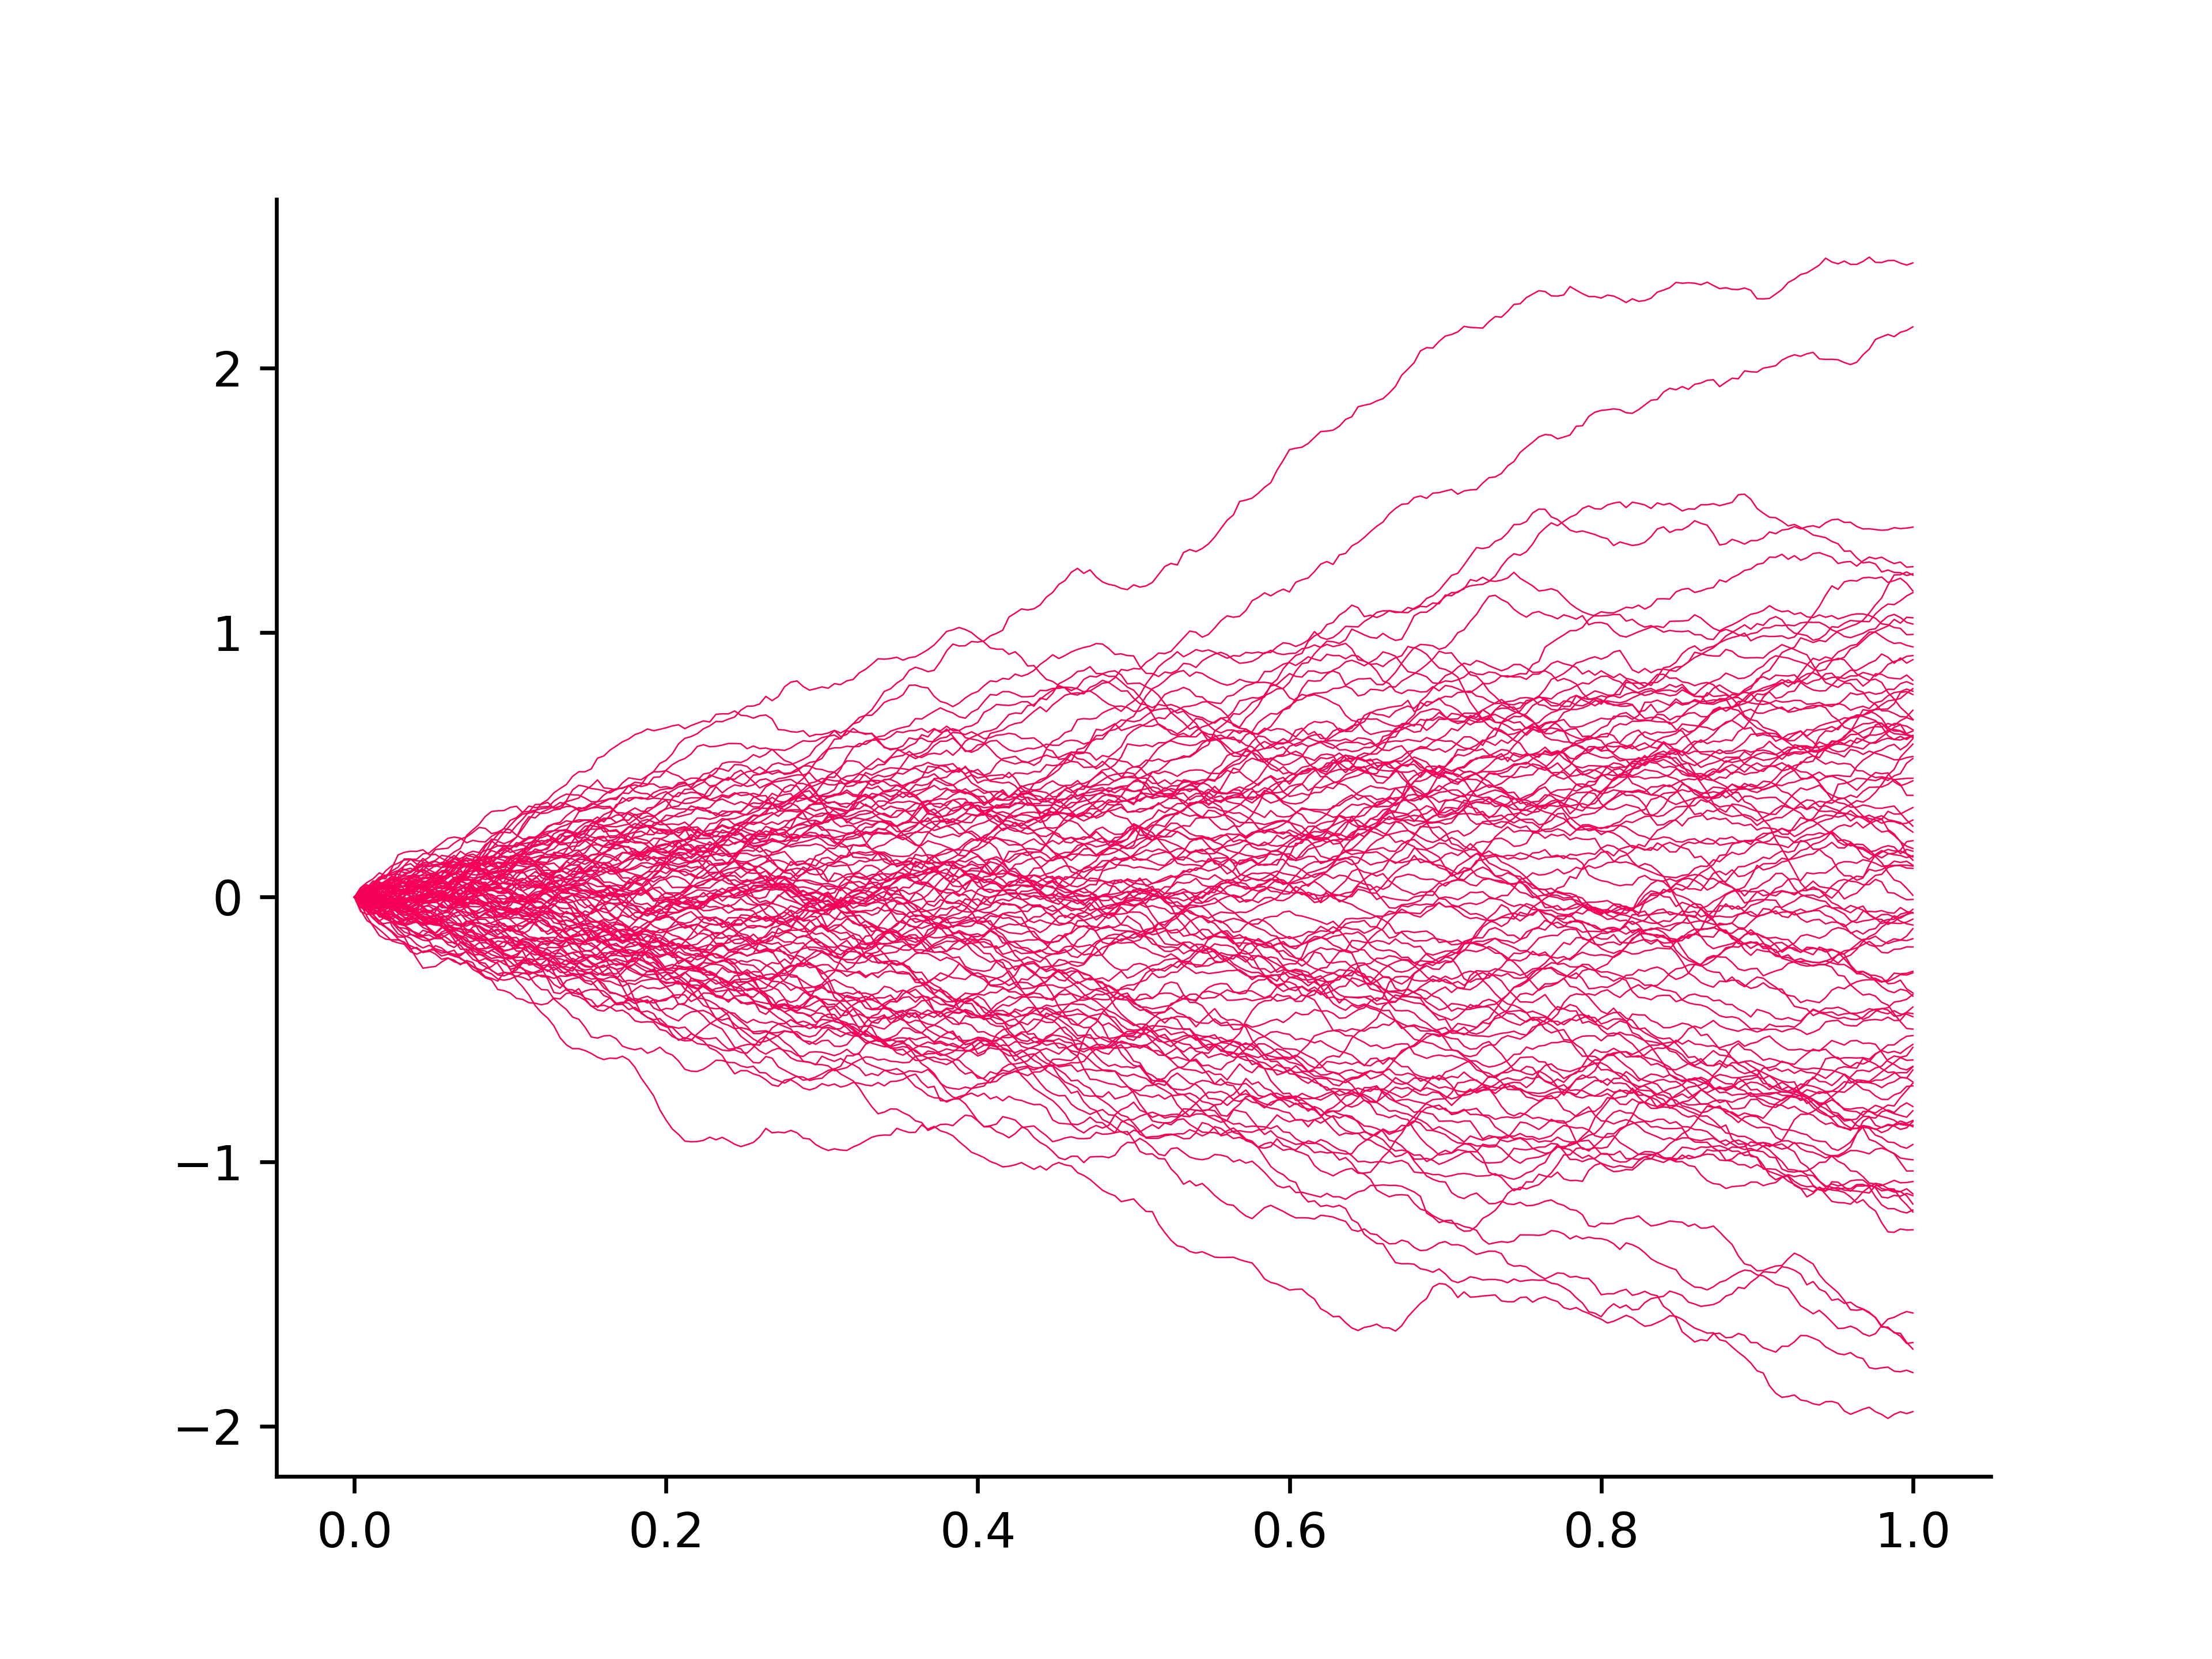
\includegraphics[scale=0.4]{image-1-75.png}
		\caption{H=0.75}
		\endminipage\hfill
	\end{figure}
	
	\begin{figure}[H]
		\minipage{0.49\textwidth}
		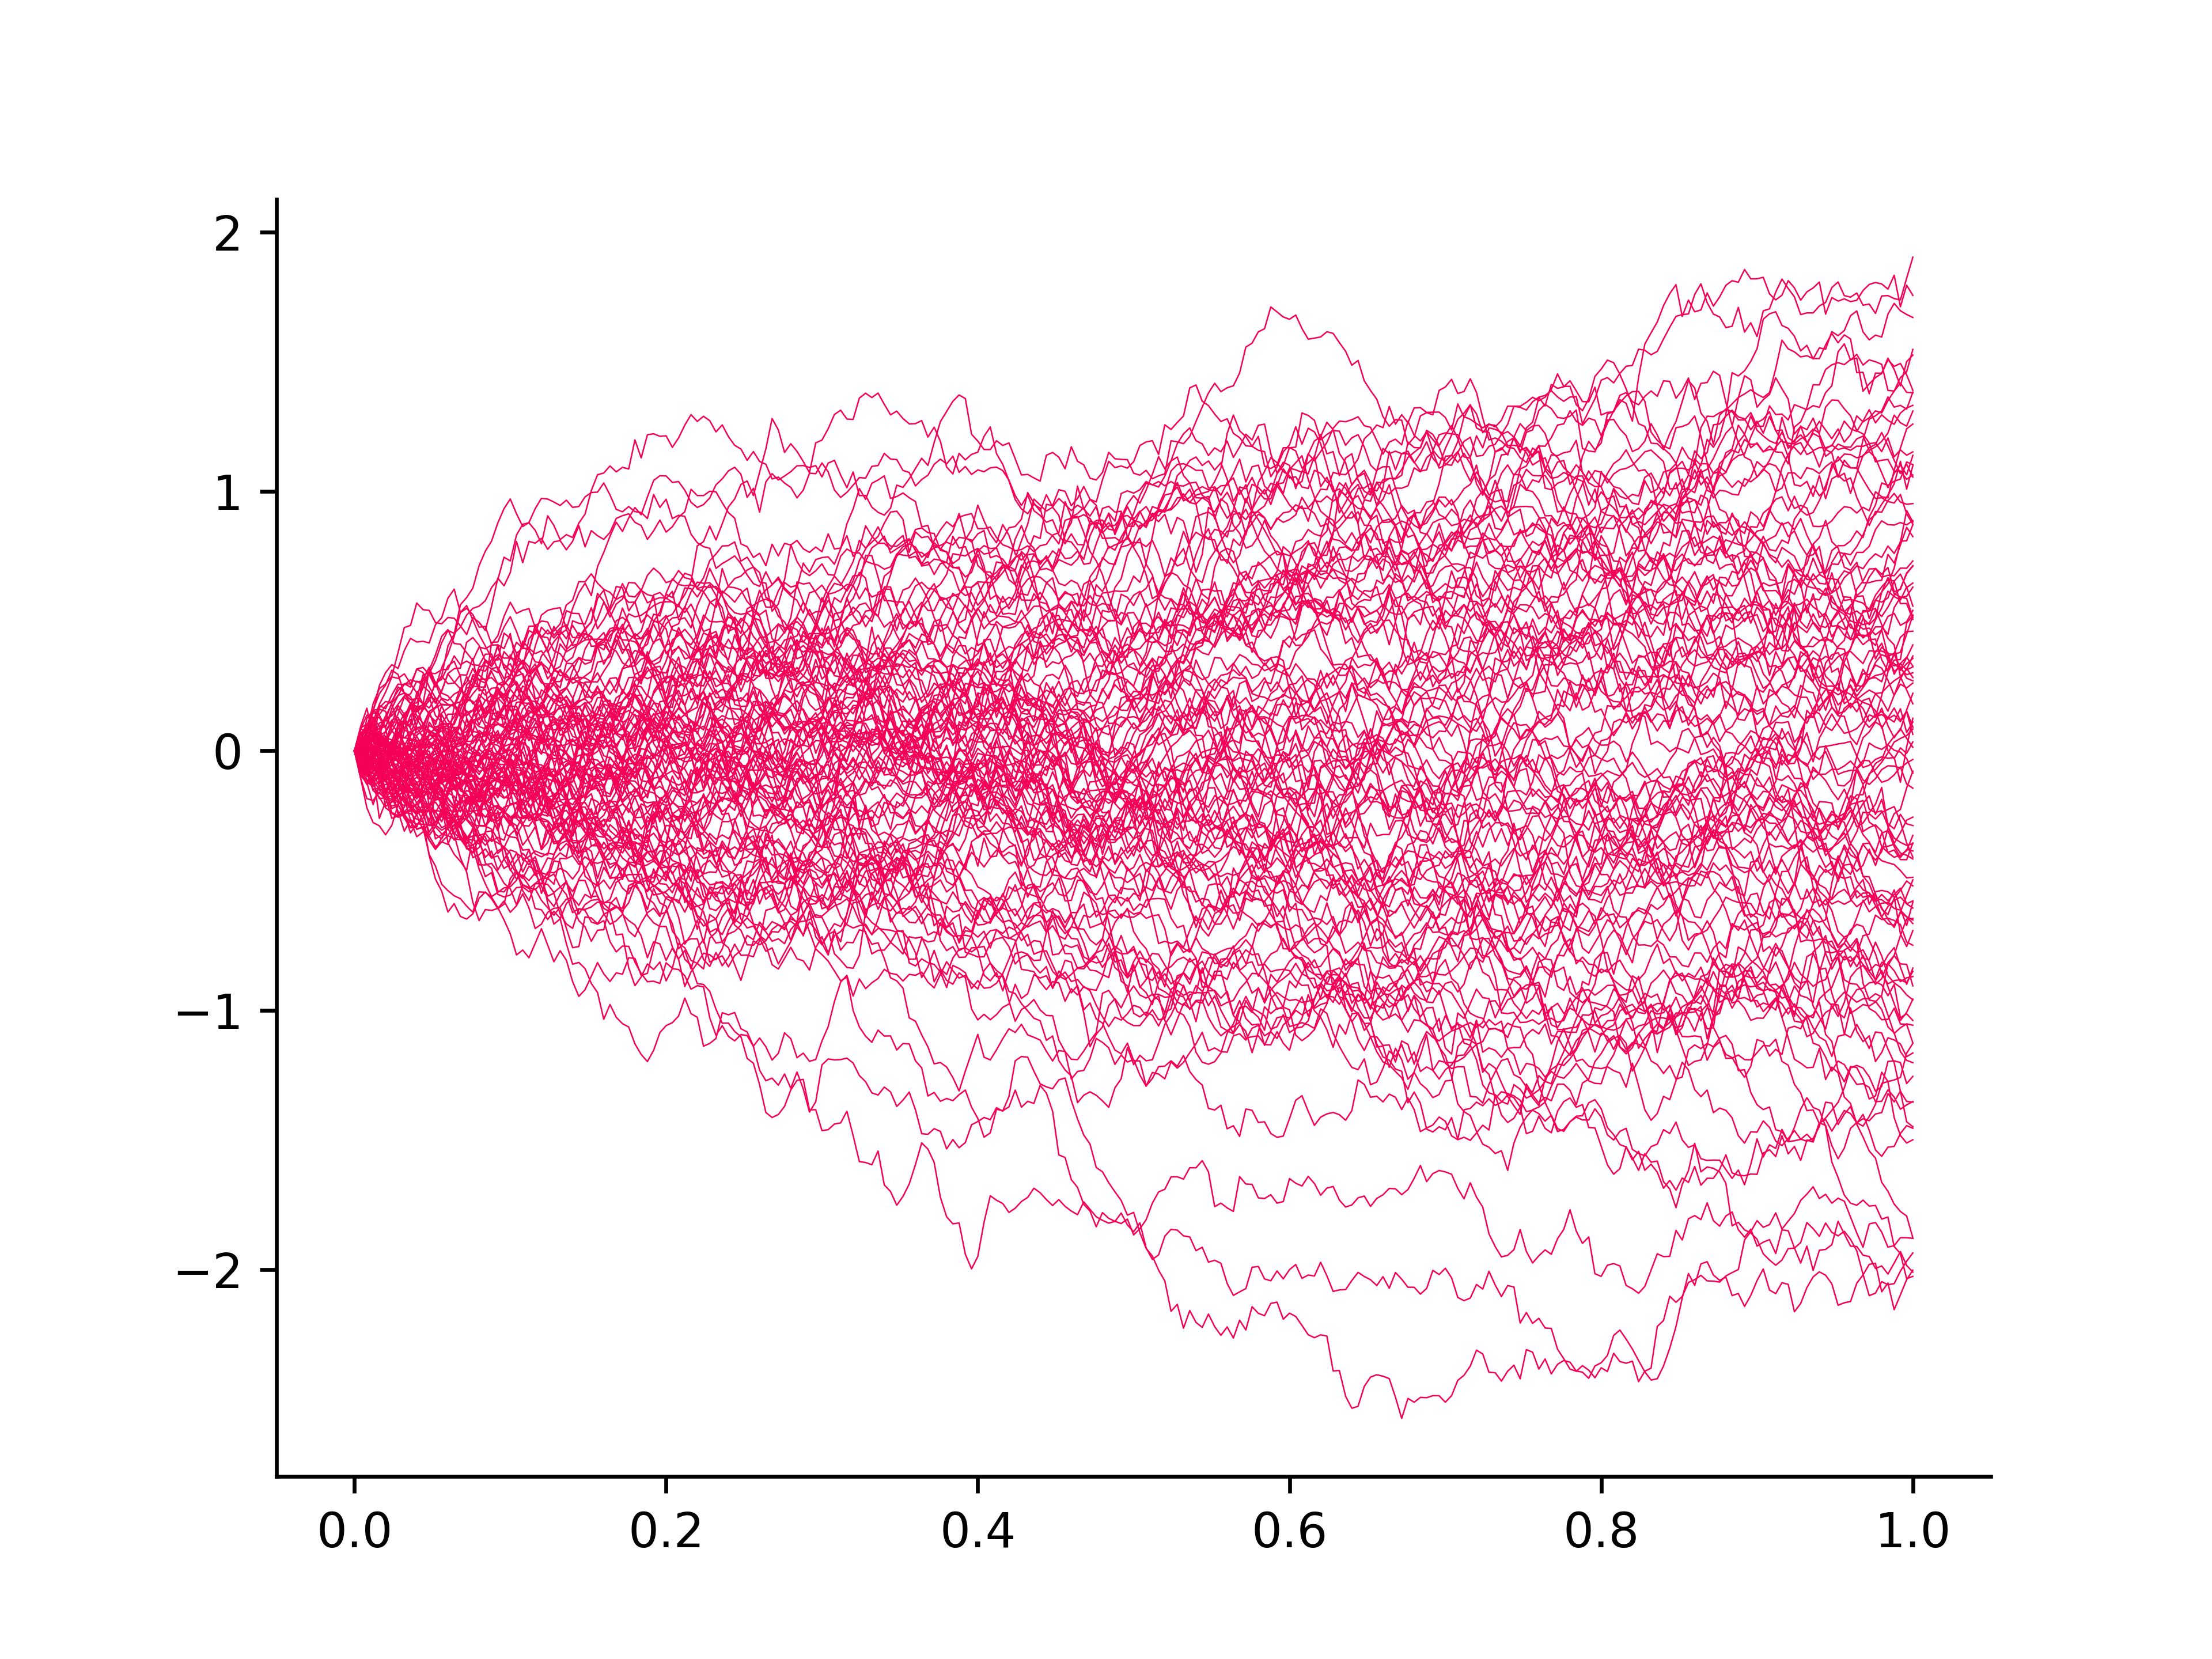
\includegraphics[scale=0.4]{image-1-55.png}
		\caption{H=0.55}
		\endminipage\hfill
		\minipage{0.49\textwidth}
		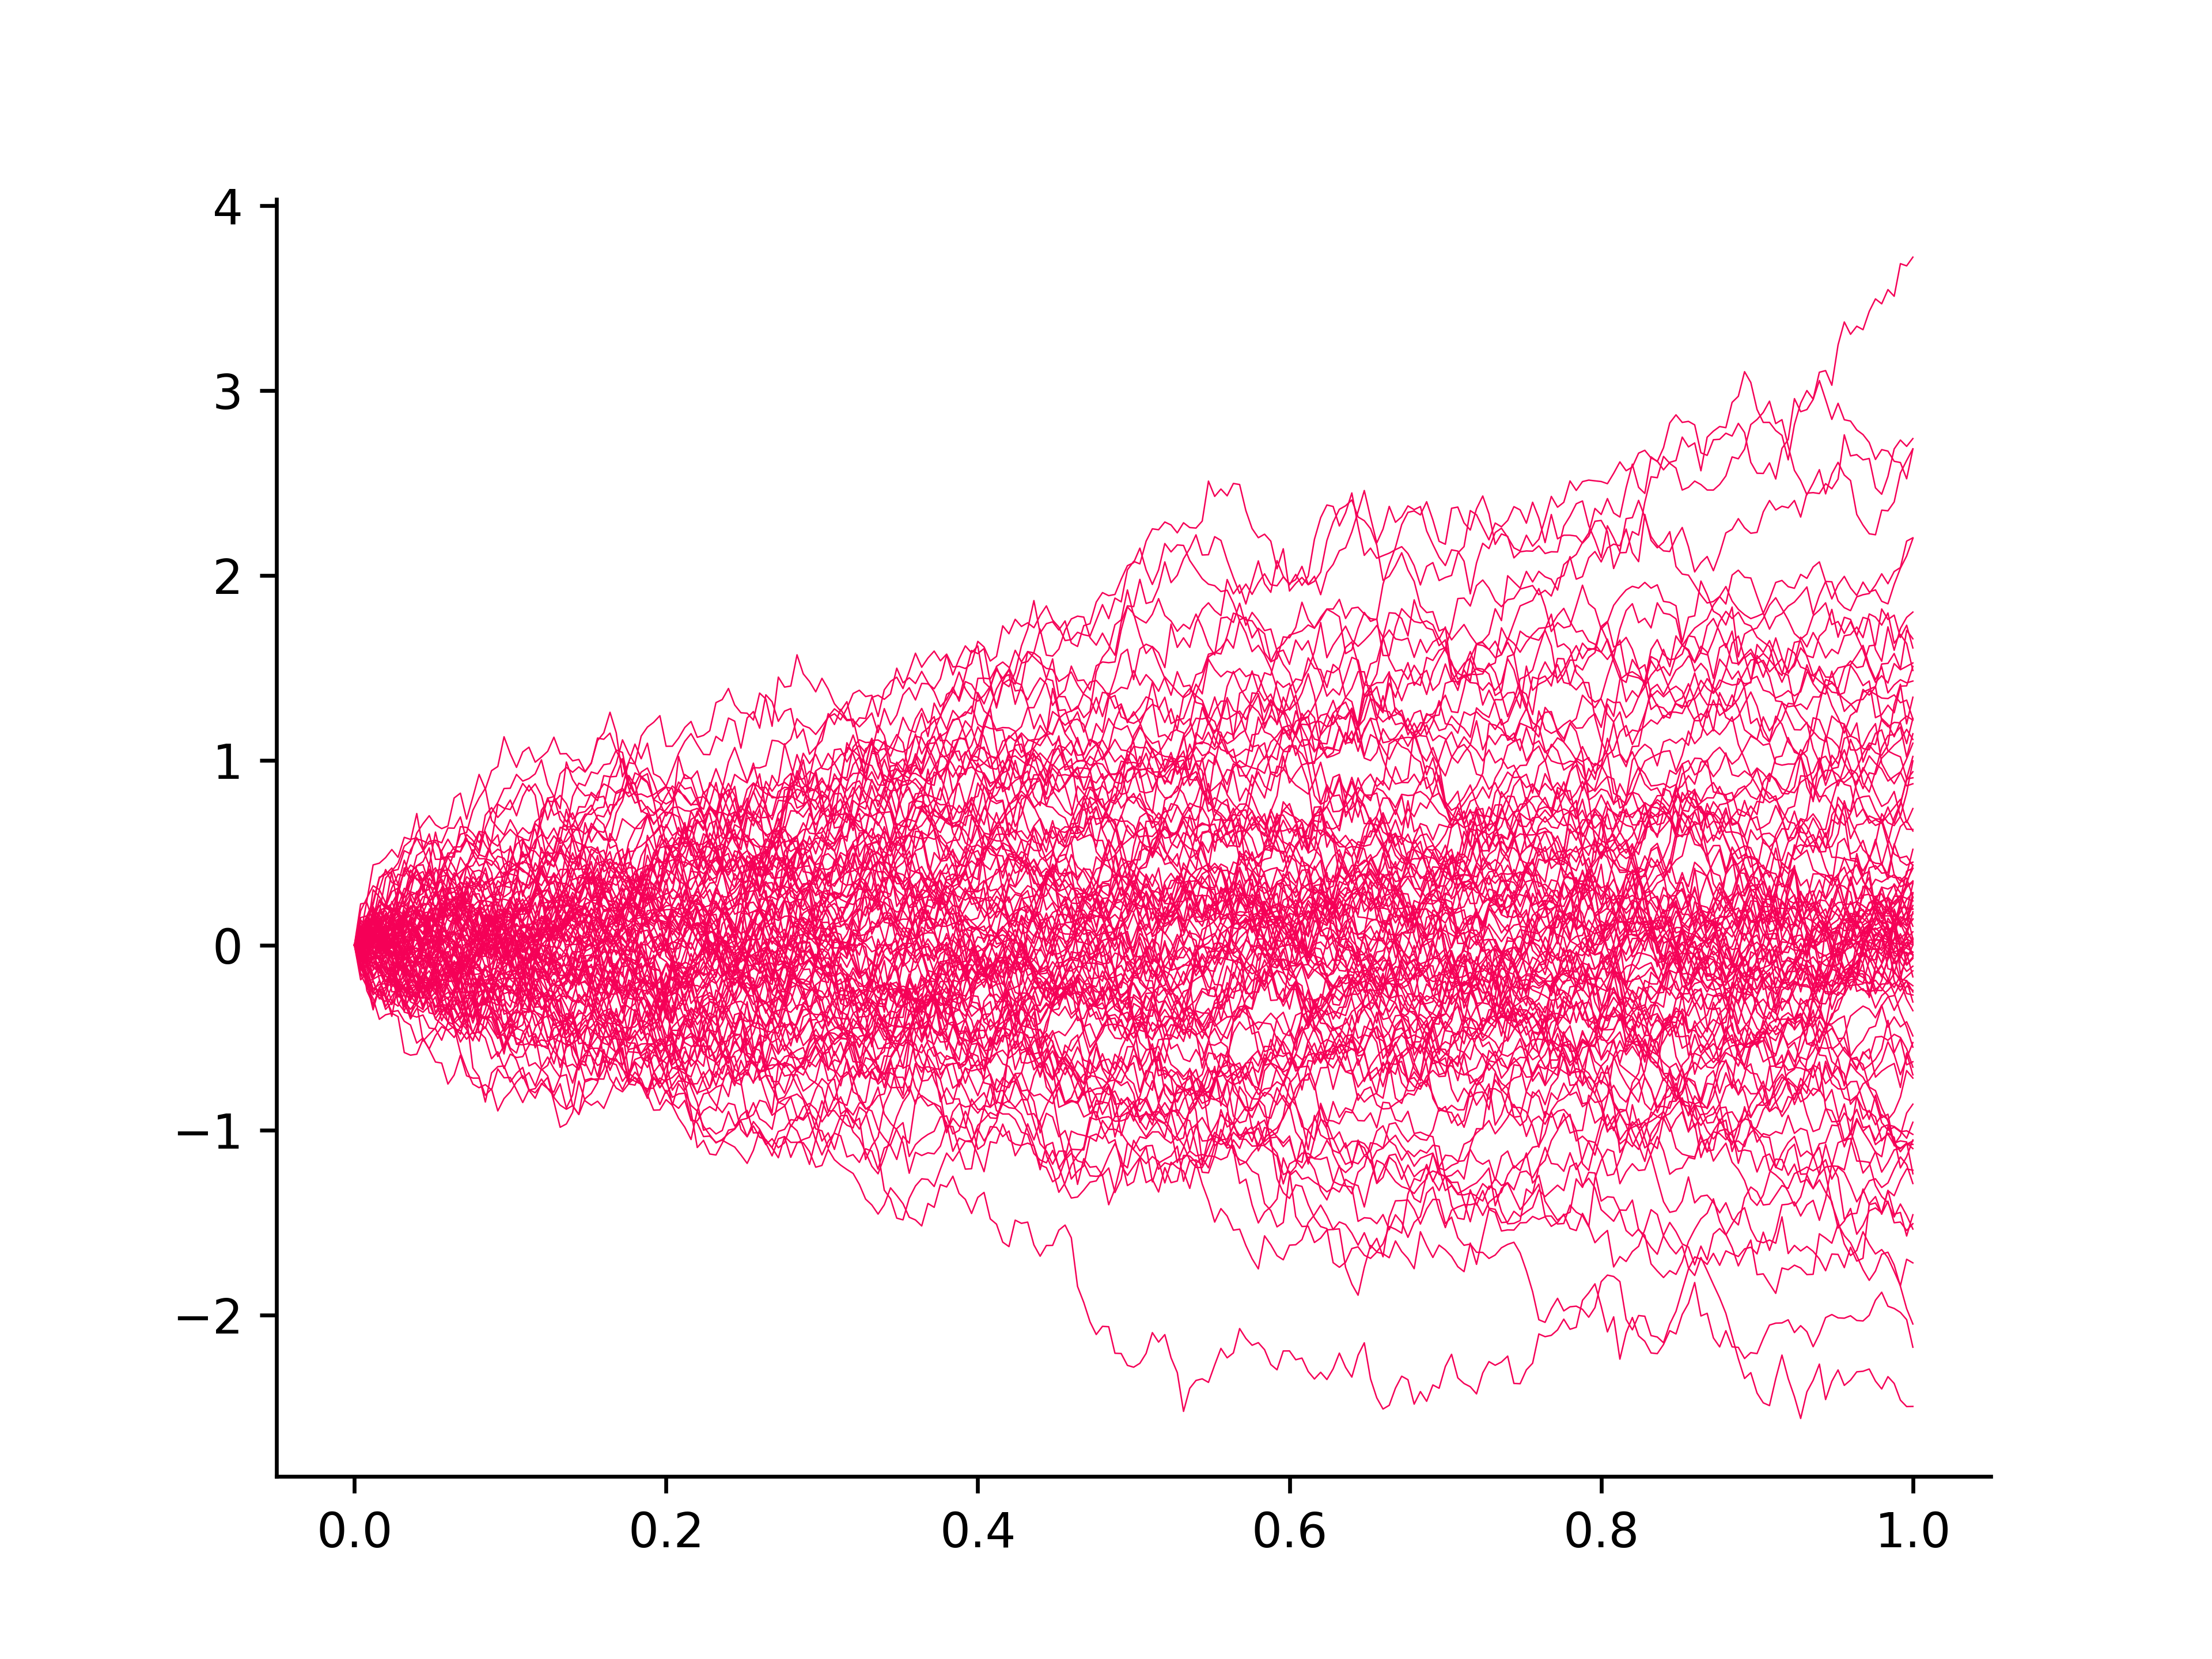
\includegraphics[scale=0.4]{image-1-45.png}
		\caption{H=0.45}
		\endminipage\hfill
	\end{figure}
	
	\begin{figure}[H]
		\minipage{0.49\textwidth}
		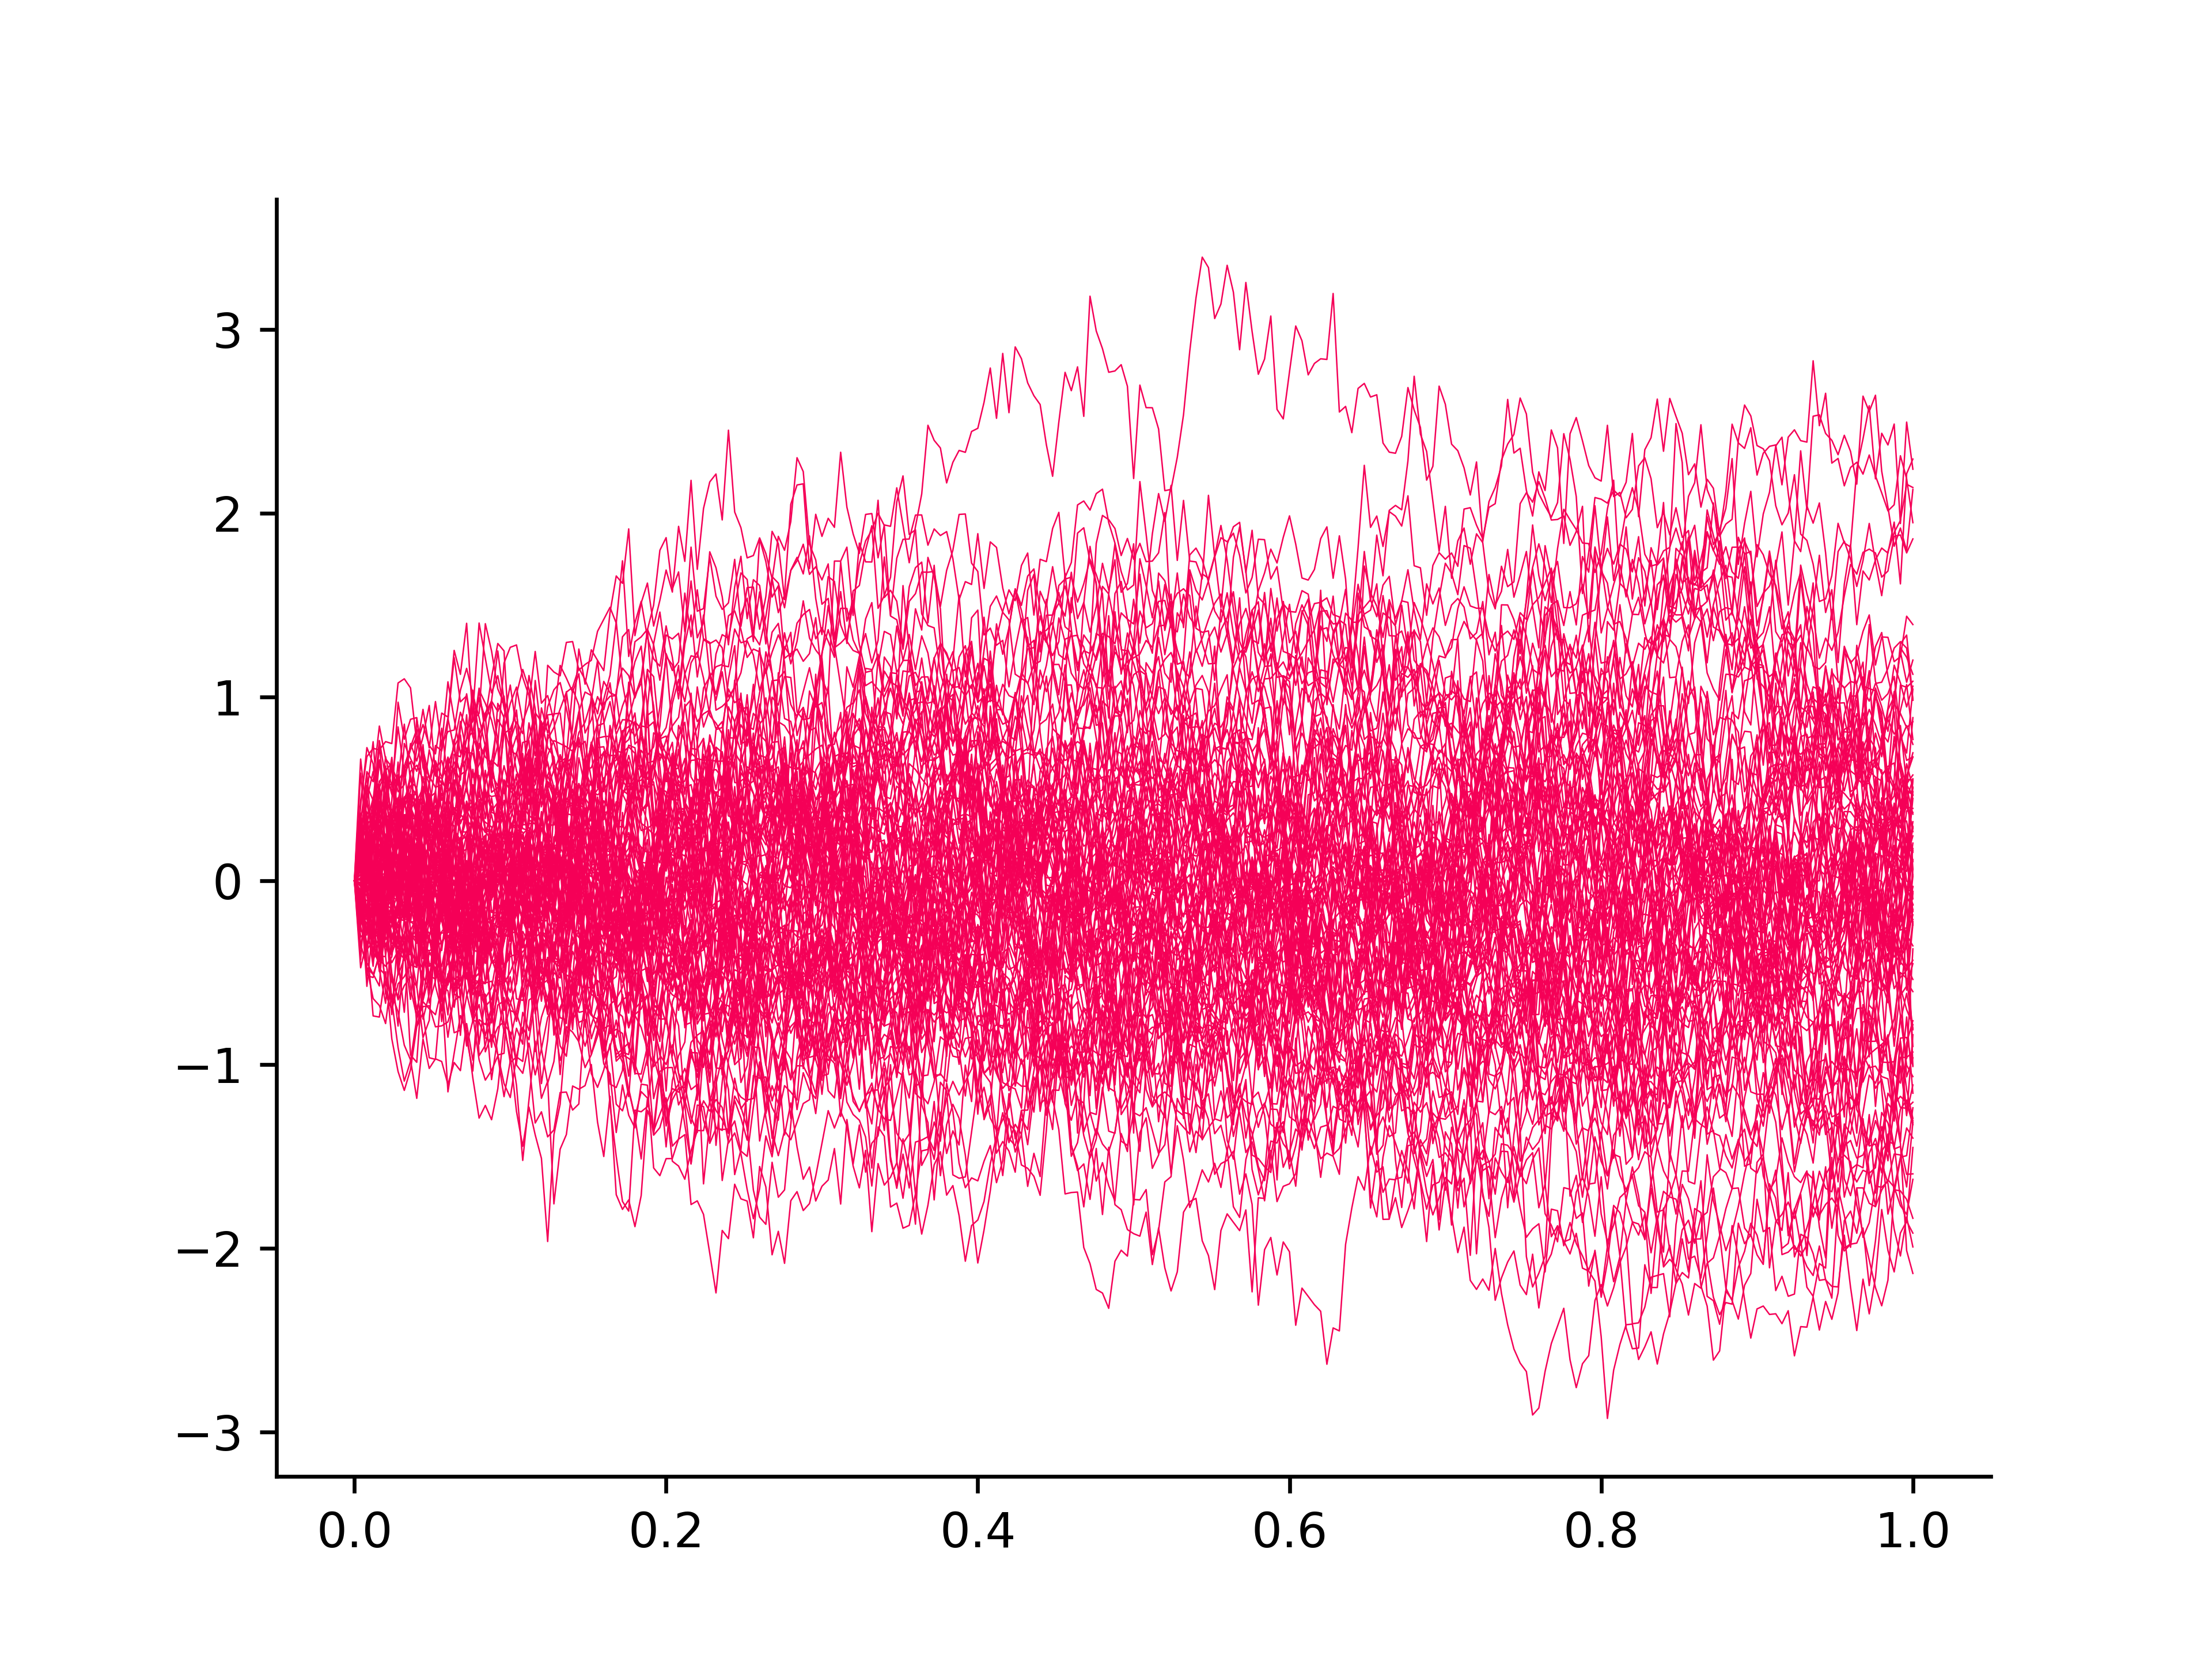
\includegraphics[scale=0.4]{image-1-25.png}
		\caption{H=0.25}
		\endminipage\hfill
		\minipage{0.49\textwidth}
		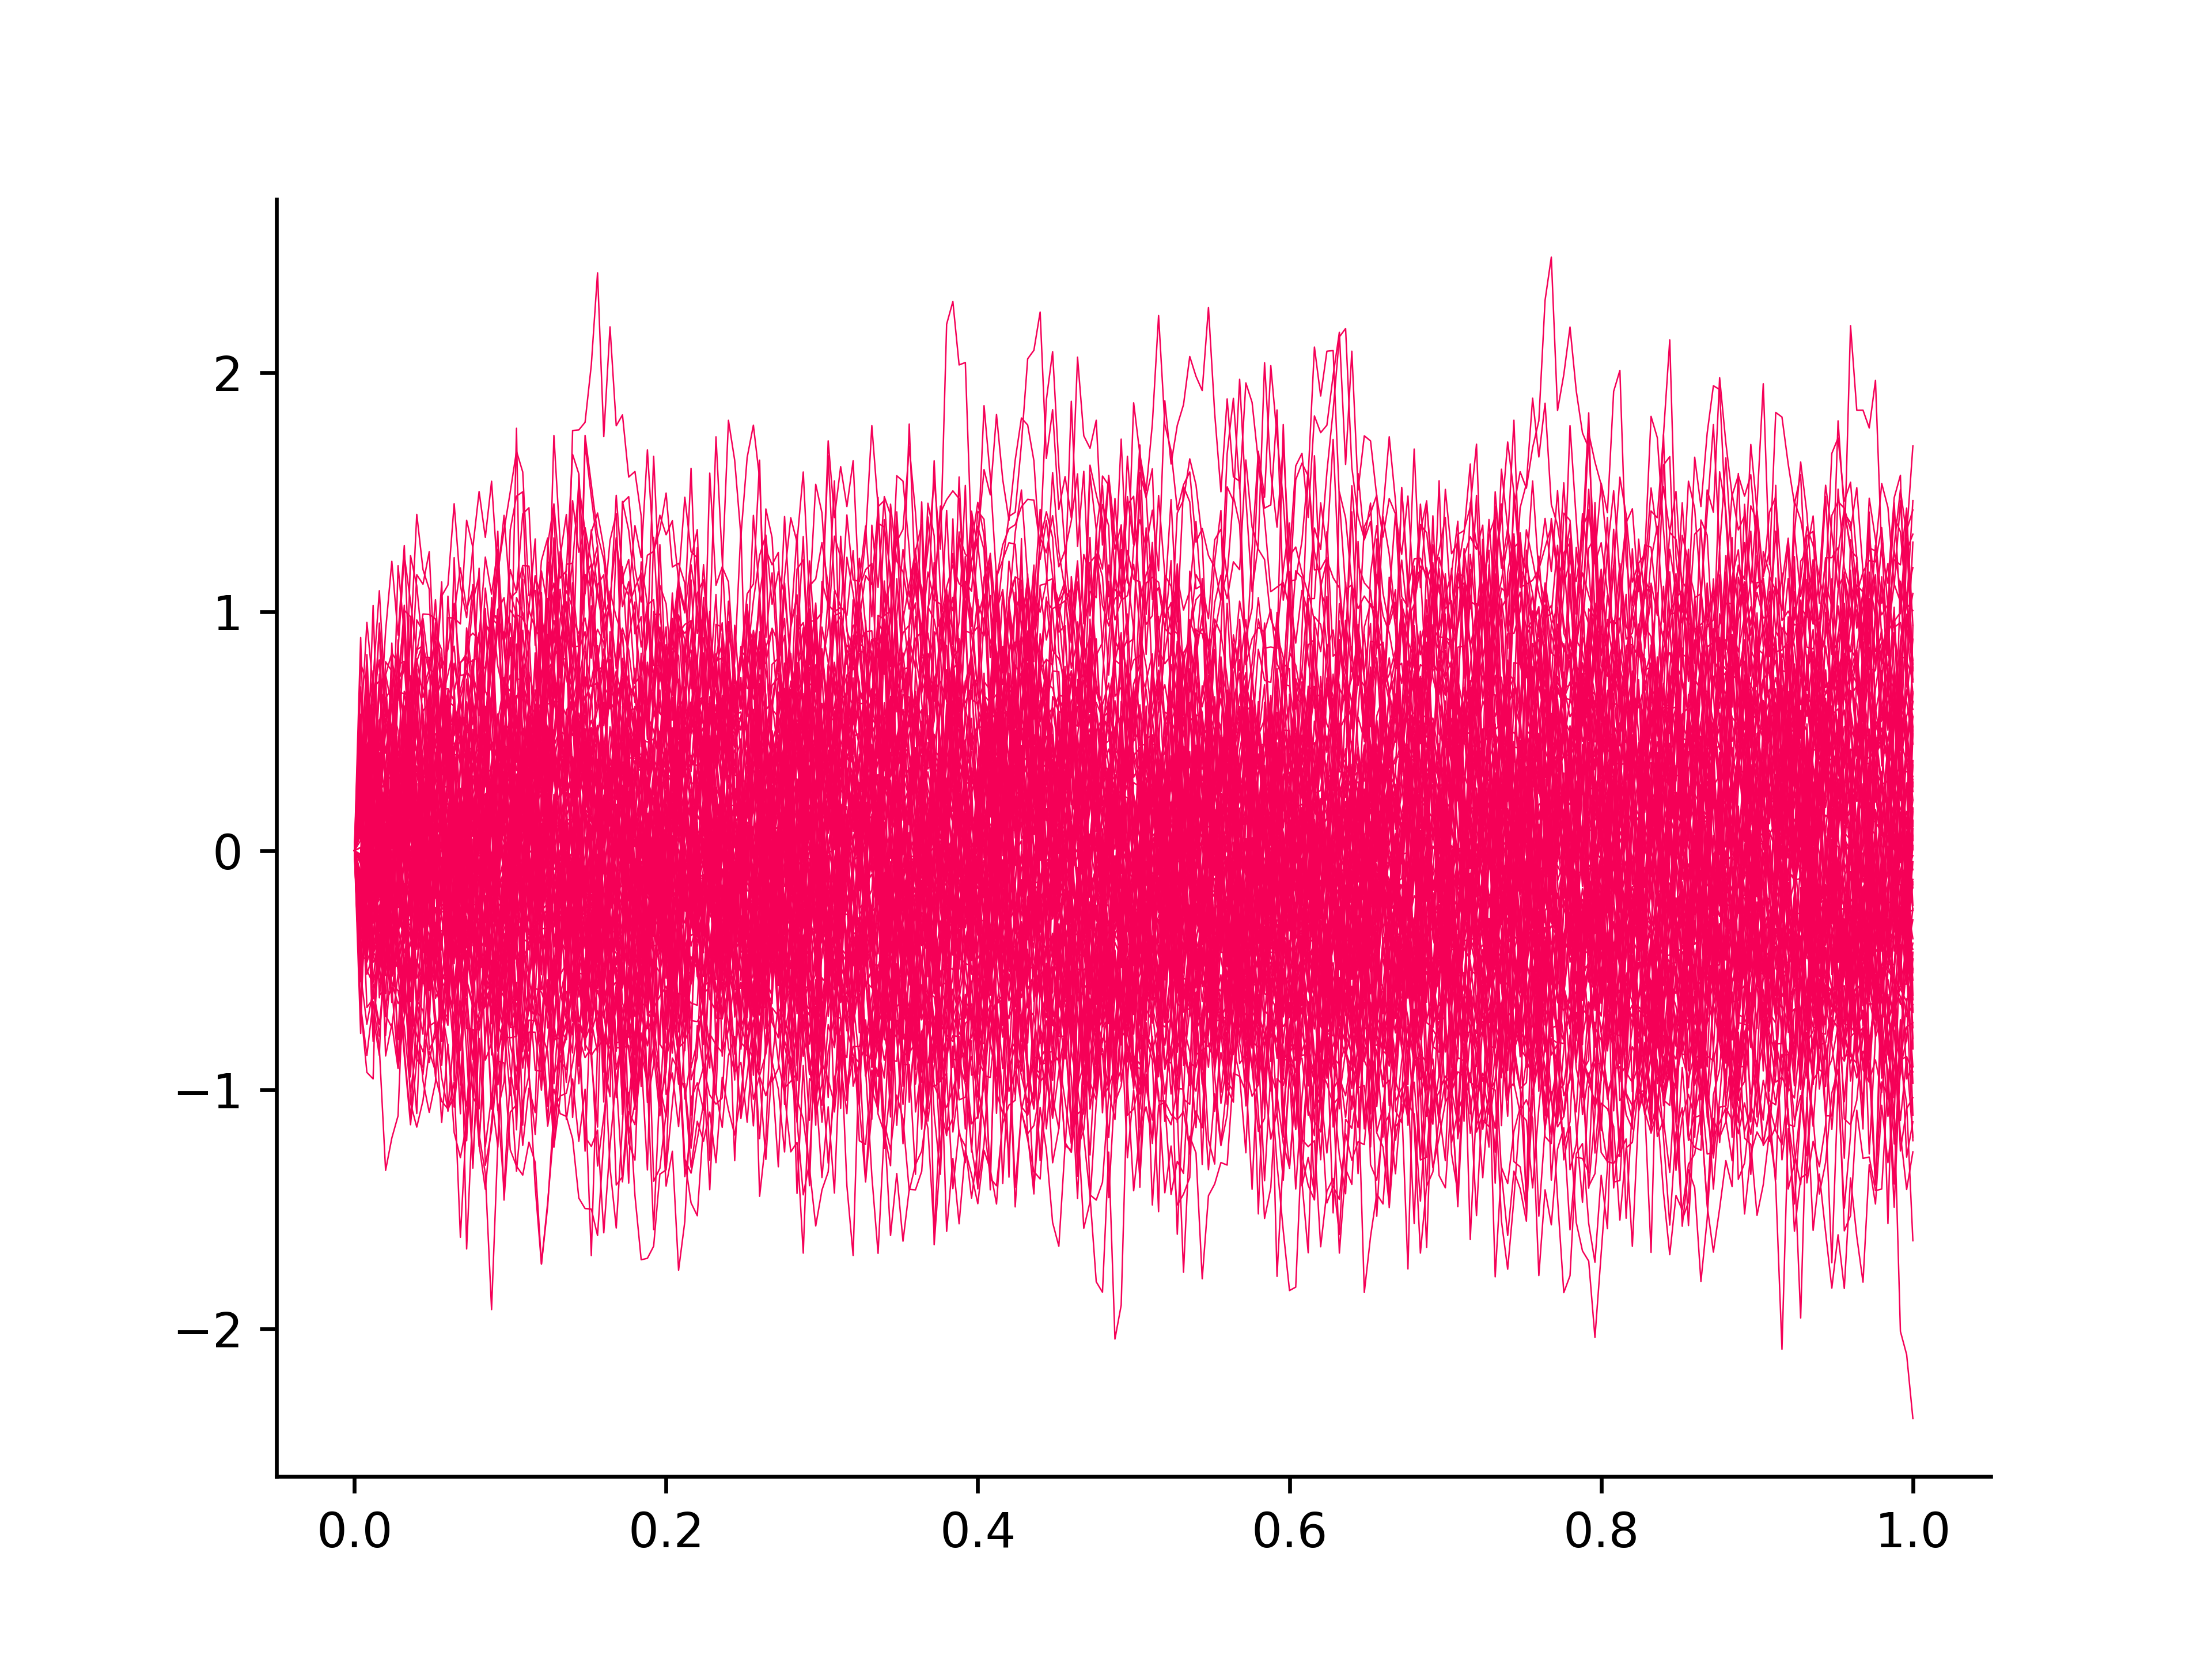
\includegraphics[scale=0.4]{image-1-05.png}
		\caption{H=0.05}
		\endminipage\hfill
	\end{figure}
	
	Не сложно вычислить выборочный коэффициент ковариации:
	\begin{figure}[H]
		\minipage{0.49\textwidth}
		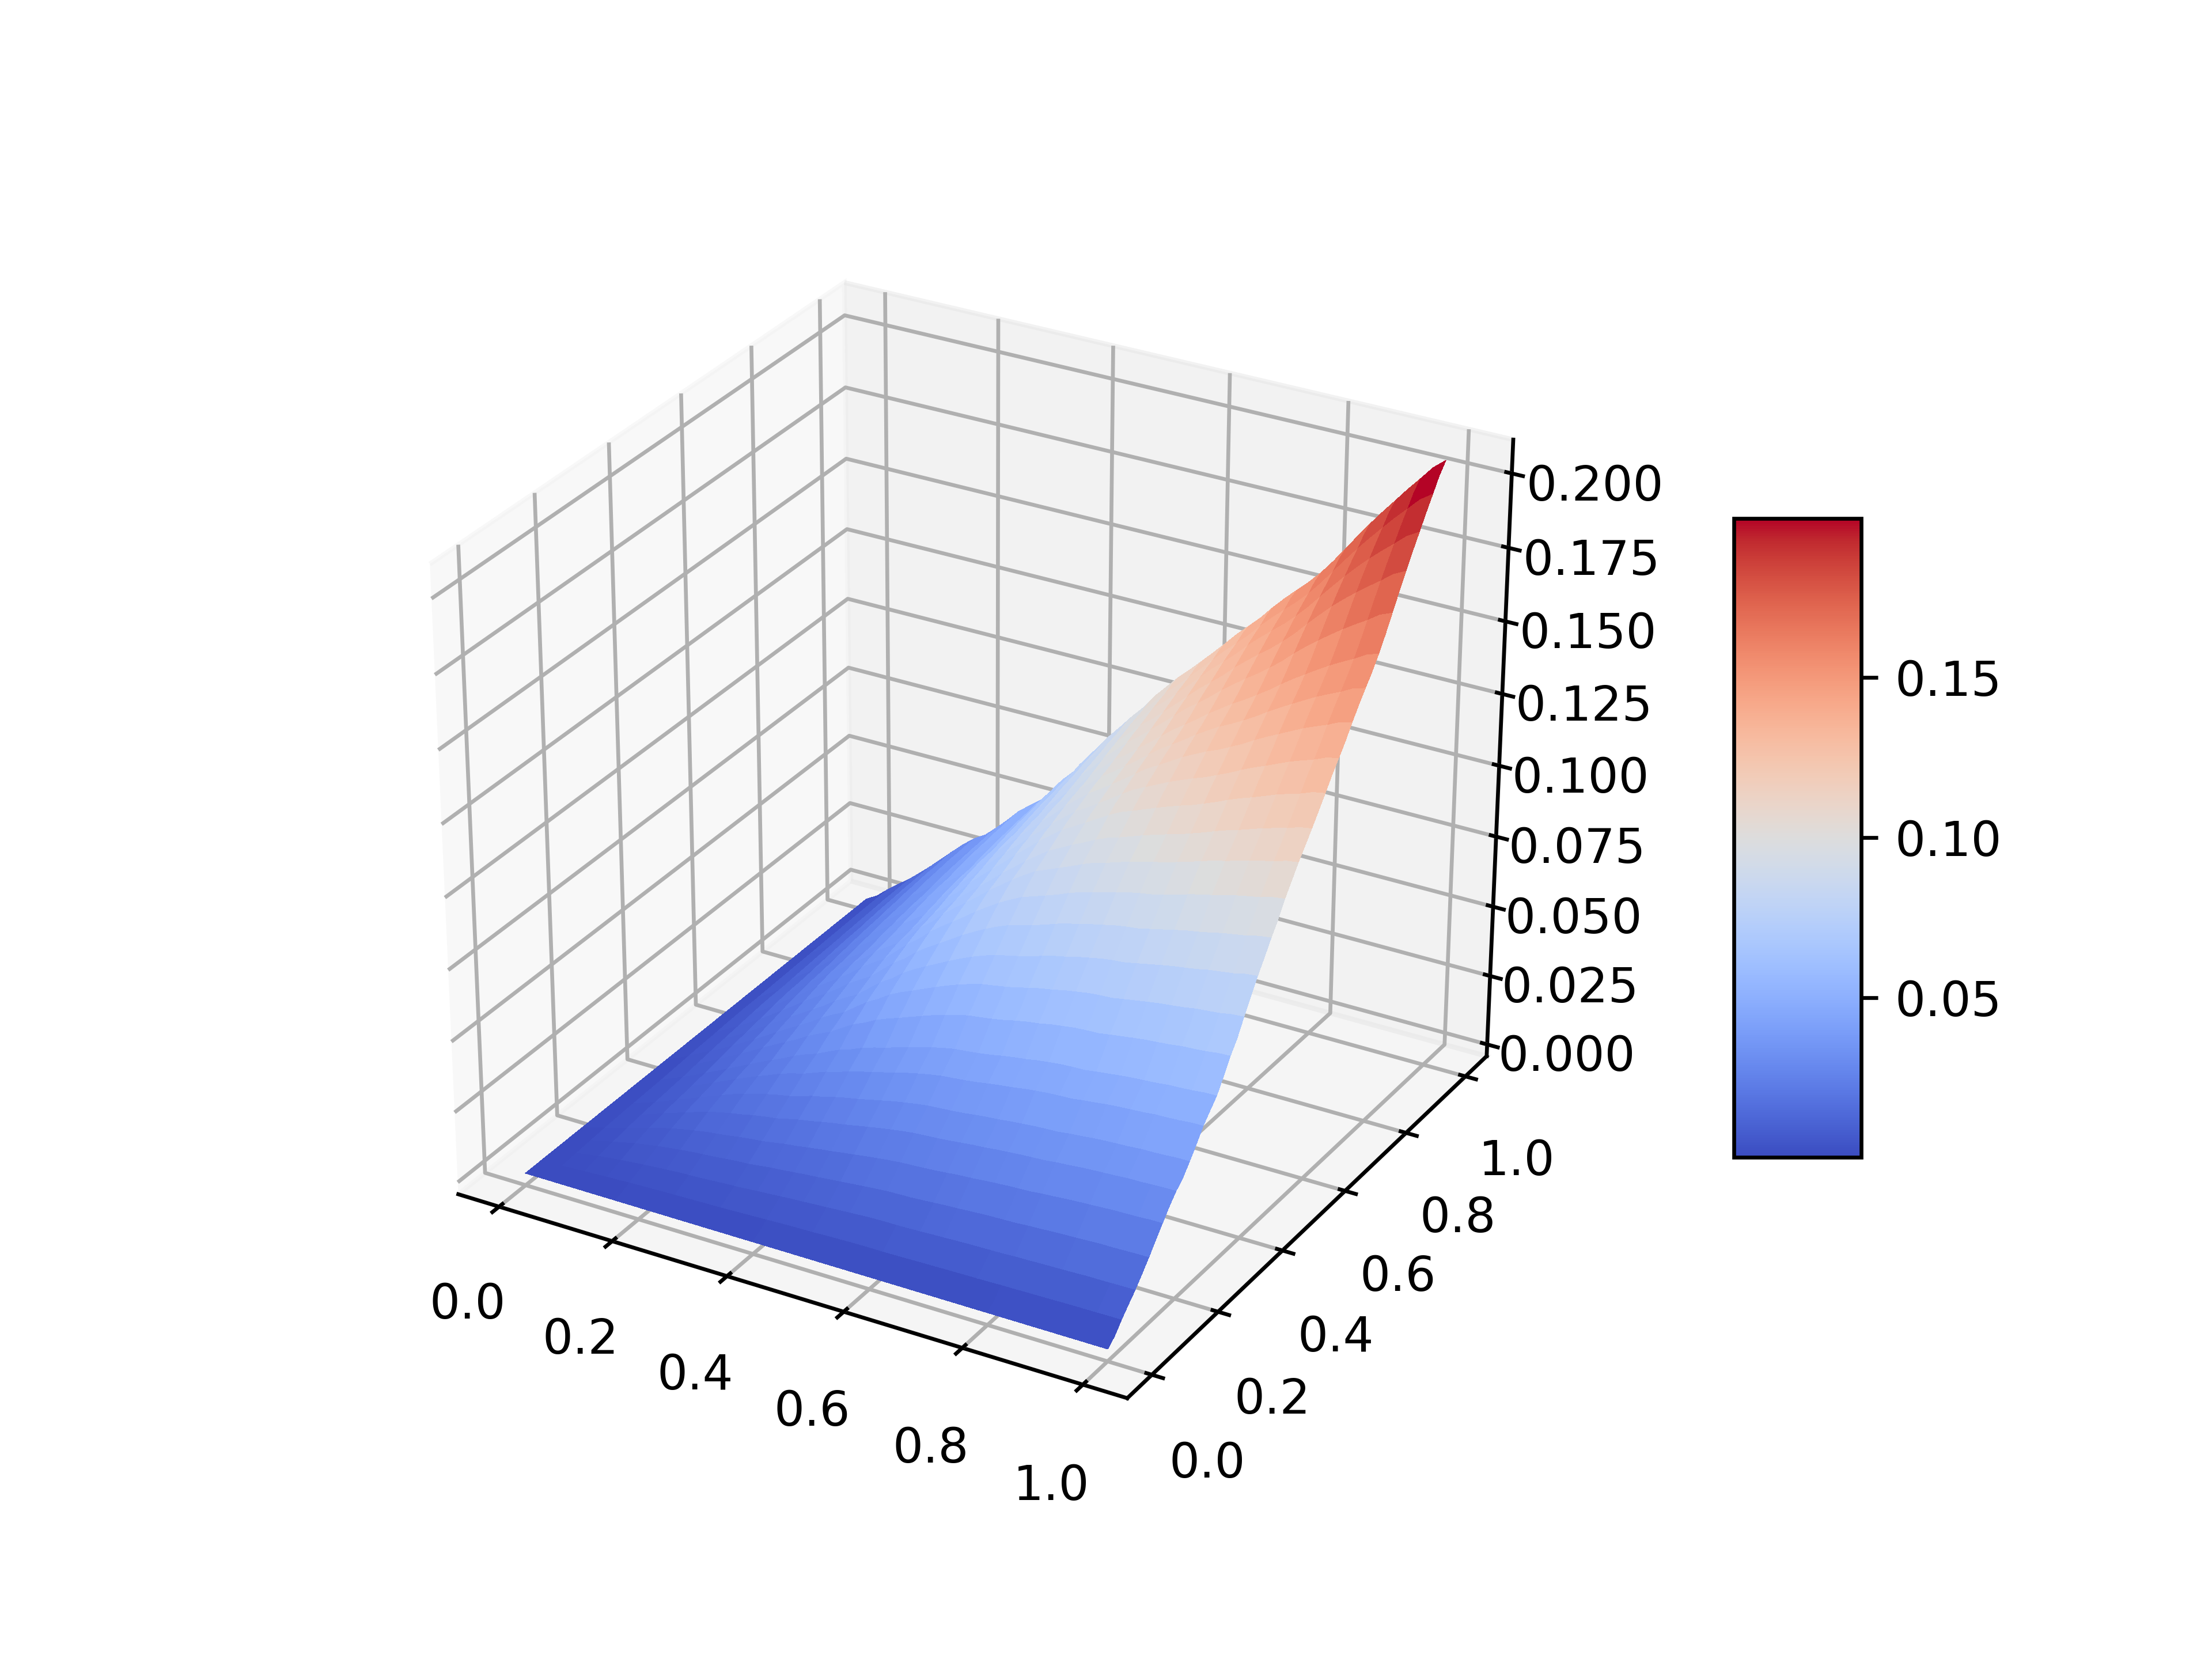
\includegraphics[scale=0.4]{covariance-1-95.png}
		\caption{H=0.95}
		\endminipage\hfill
		\minipage{0.49\textwidth}
		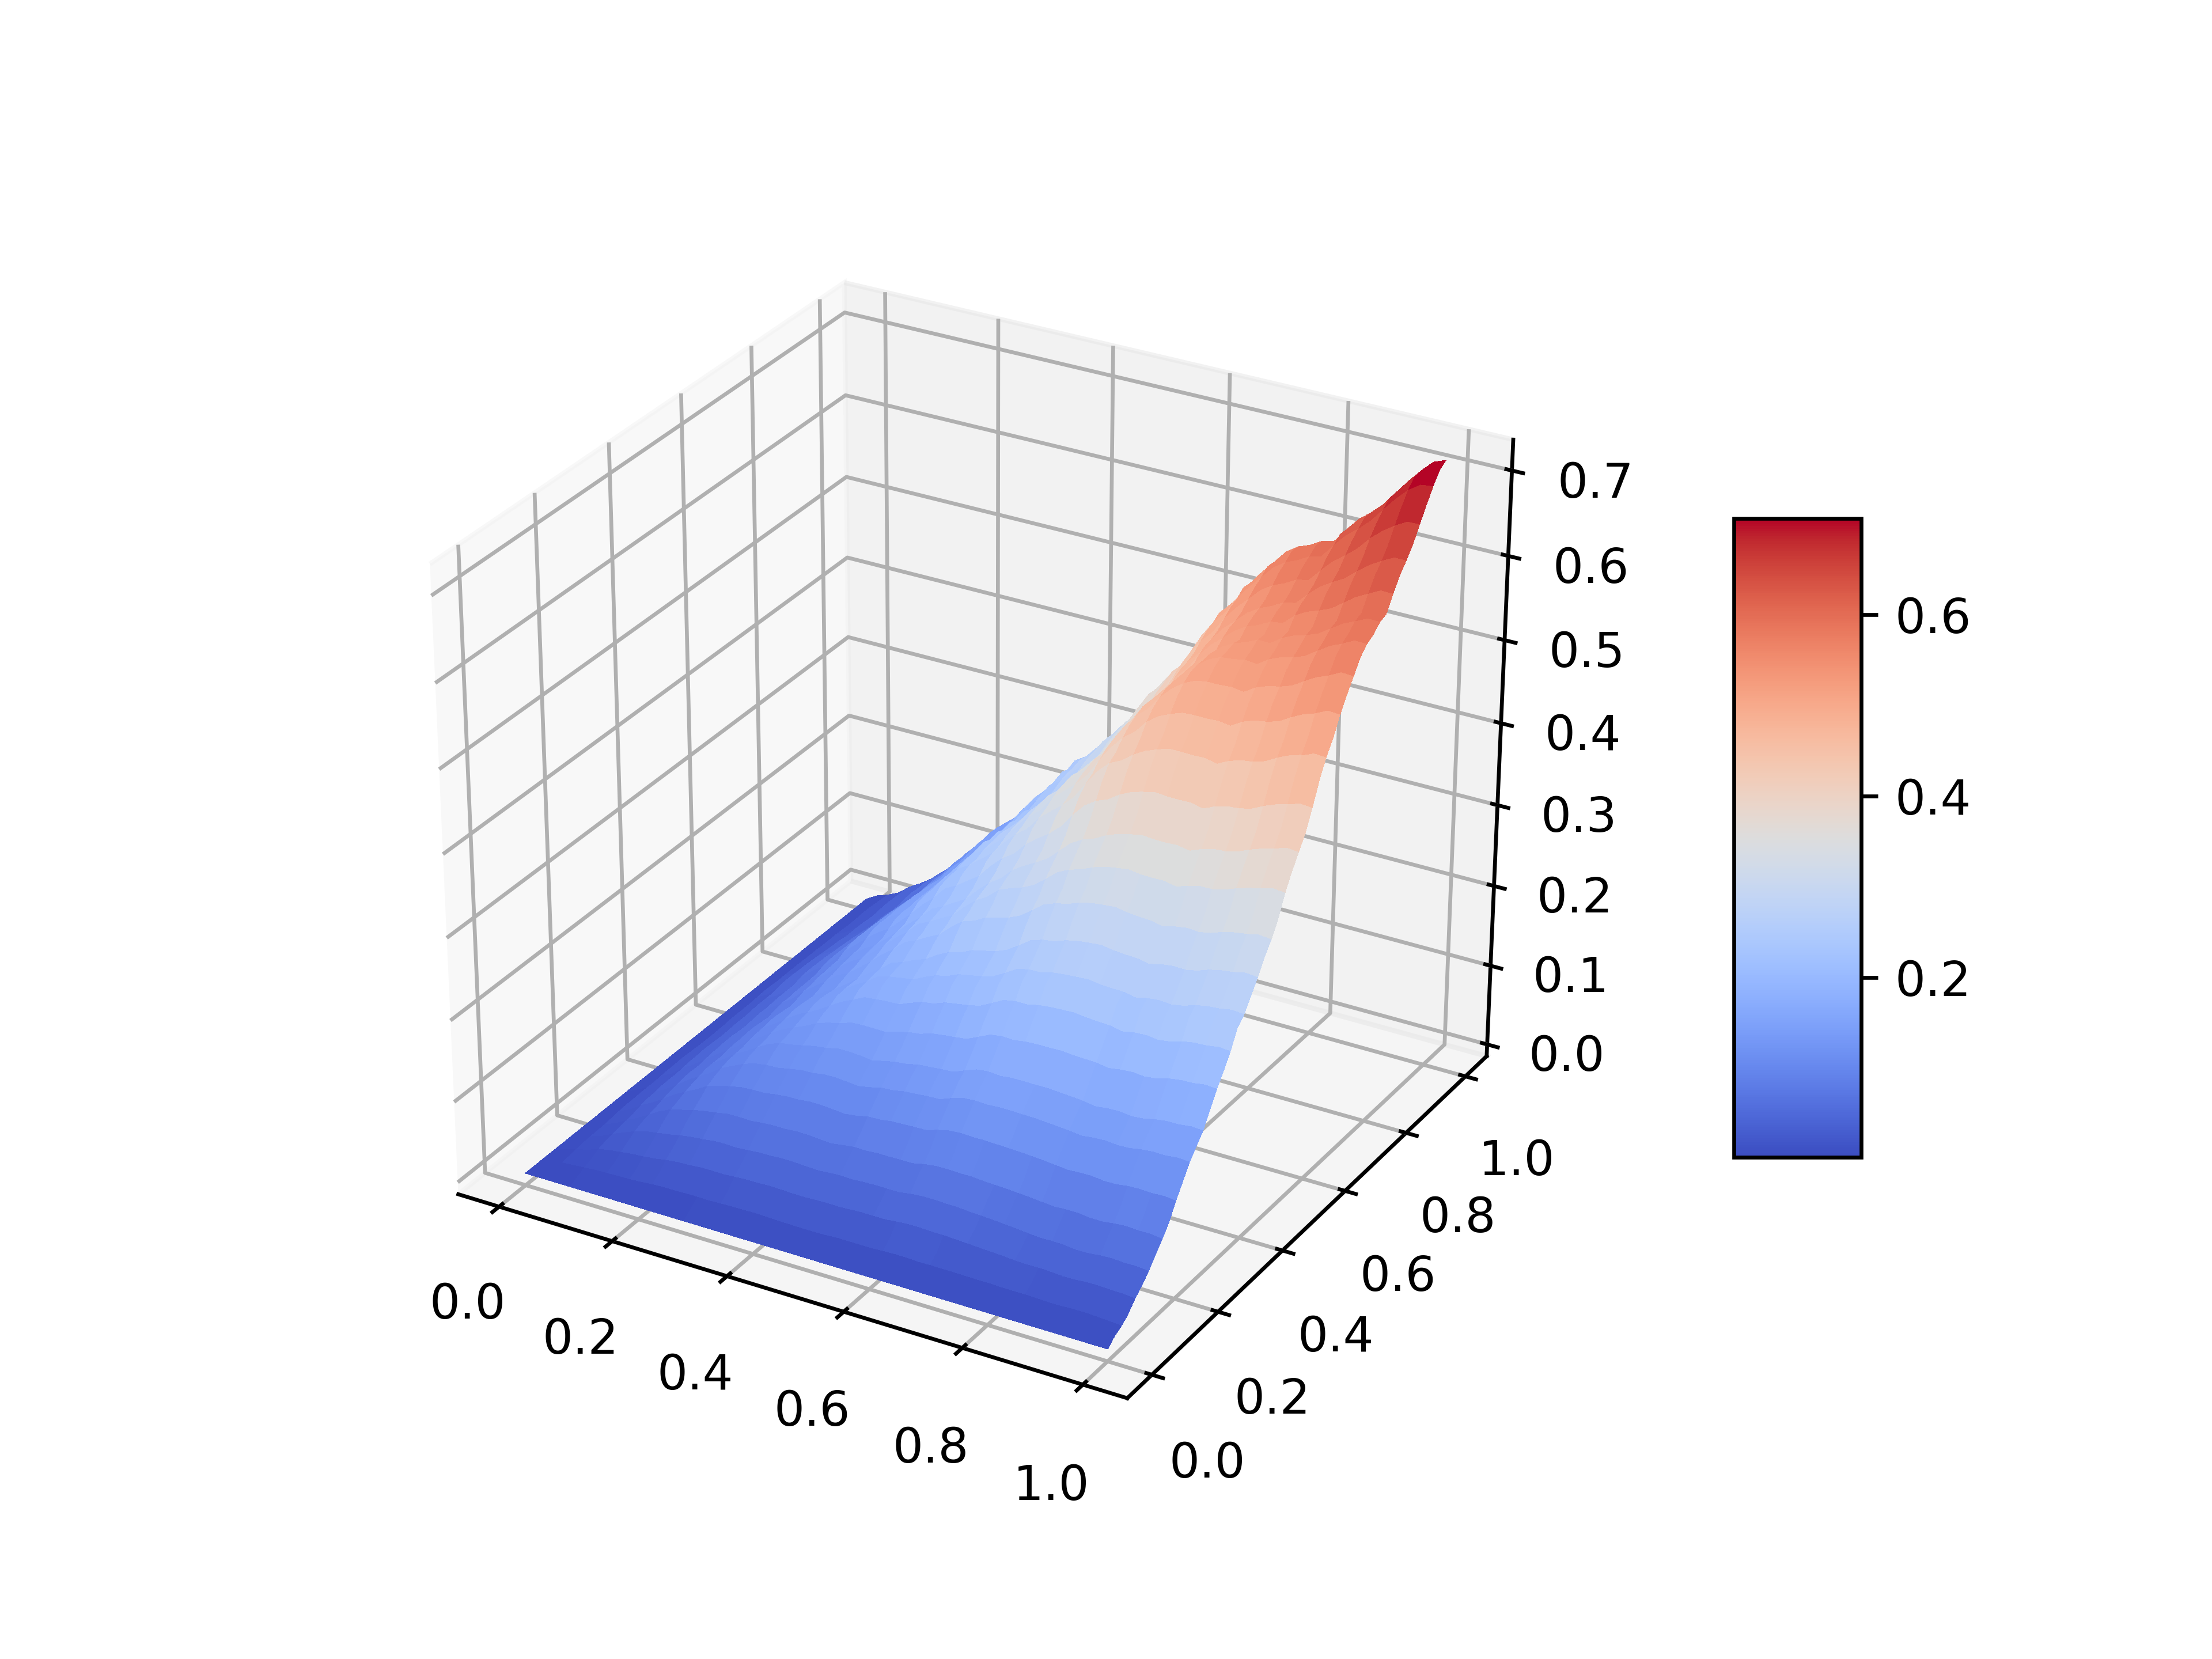
\includegraphics[scale=0.4]{covariance-1-75.png}
		\caption{H=0.75}
		\endminipage\hfill
	\end{figure}
	
	\begin{figure}[H]
		\minipage{0.49\textwidth}
		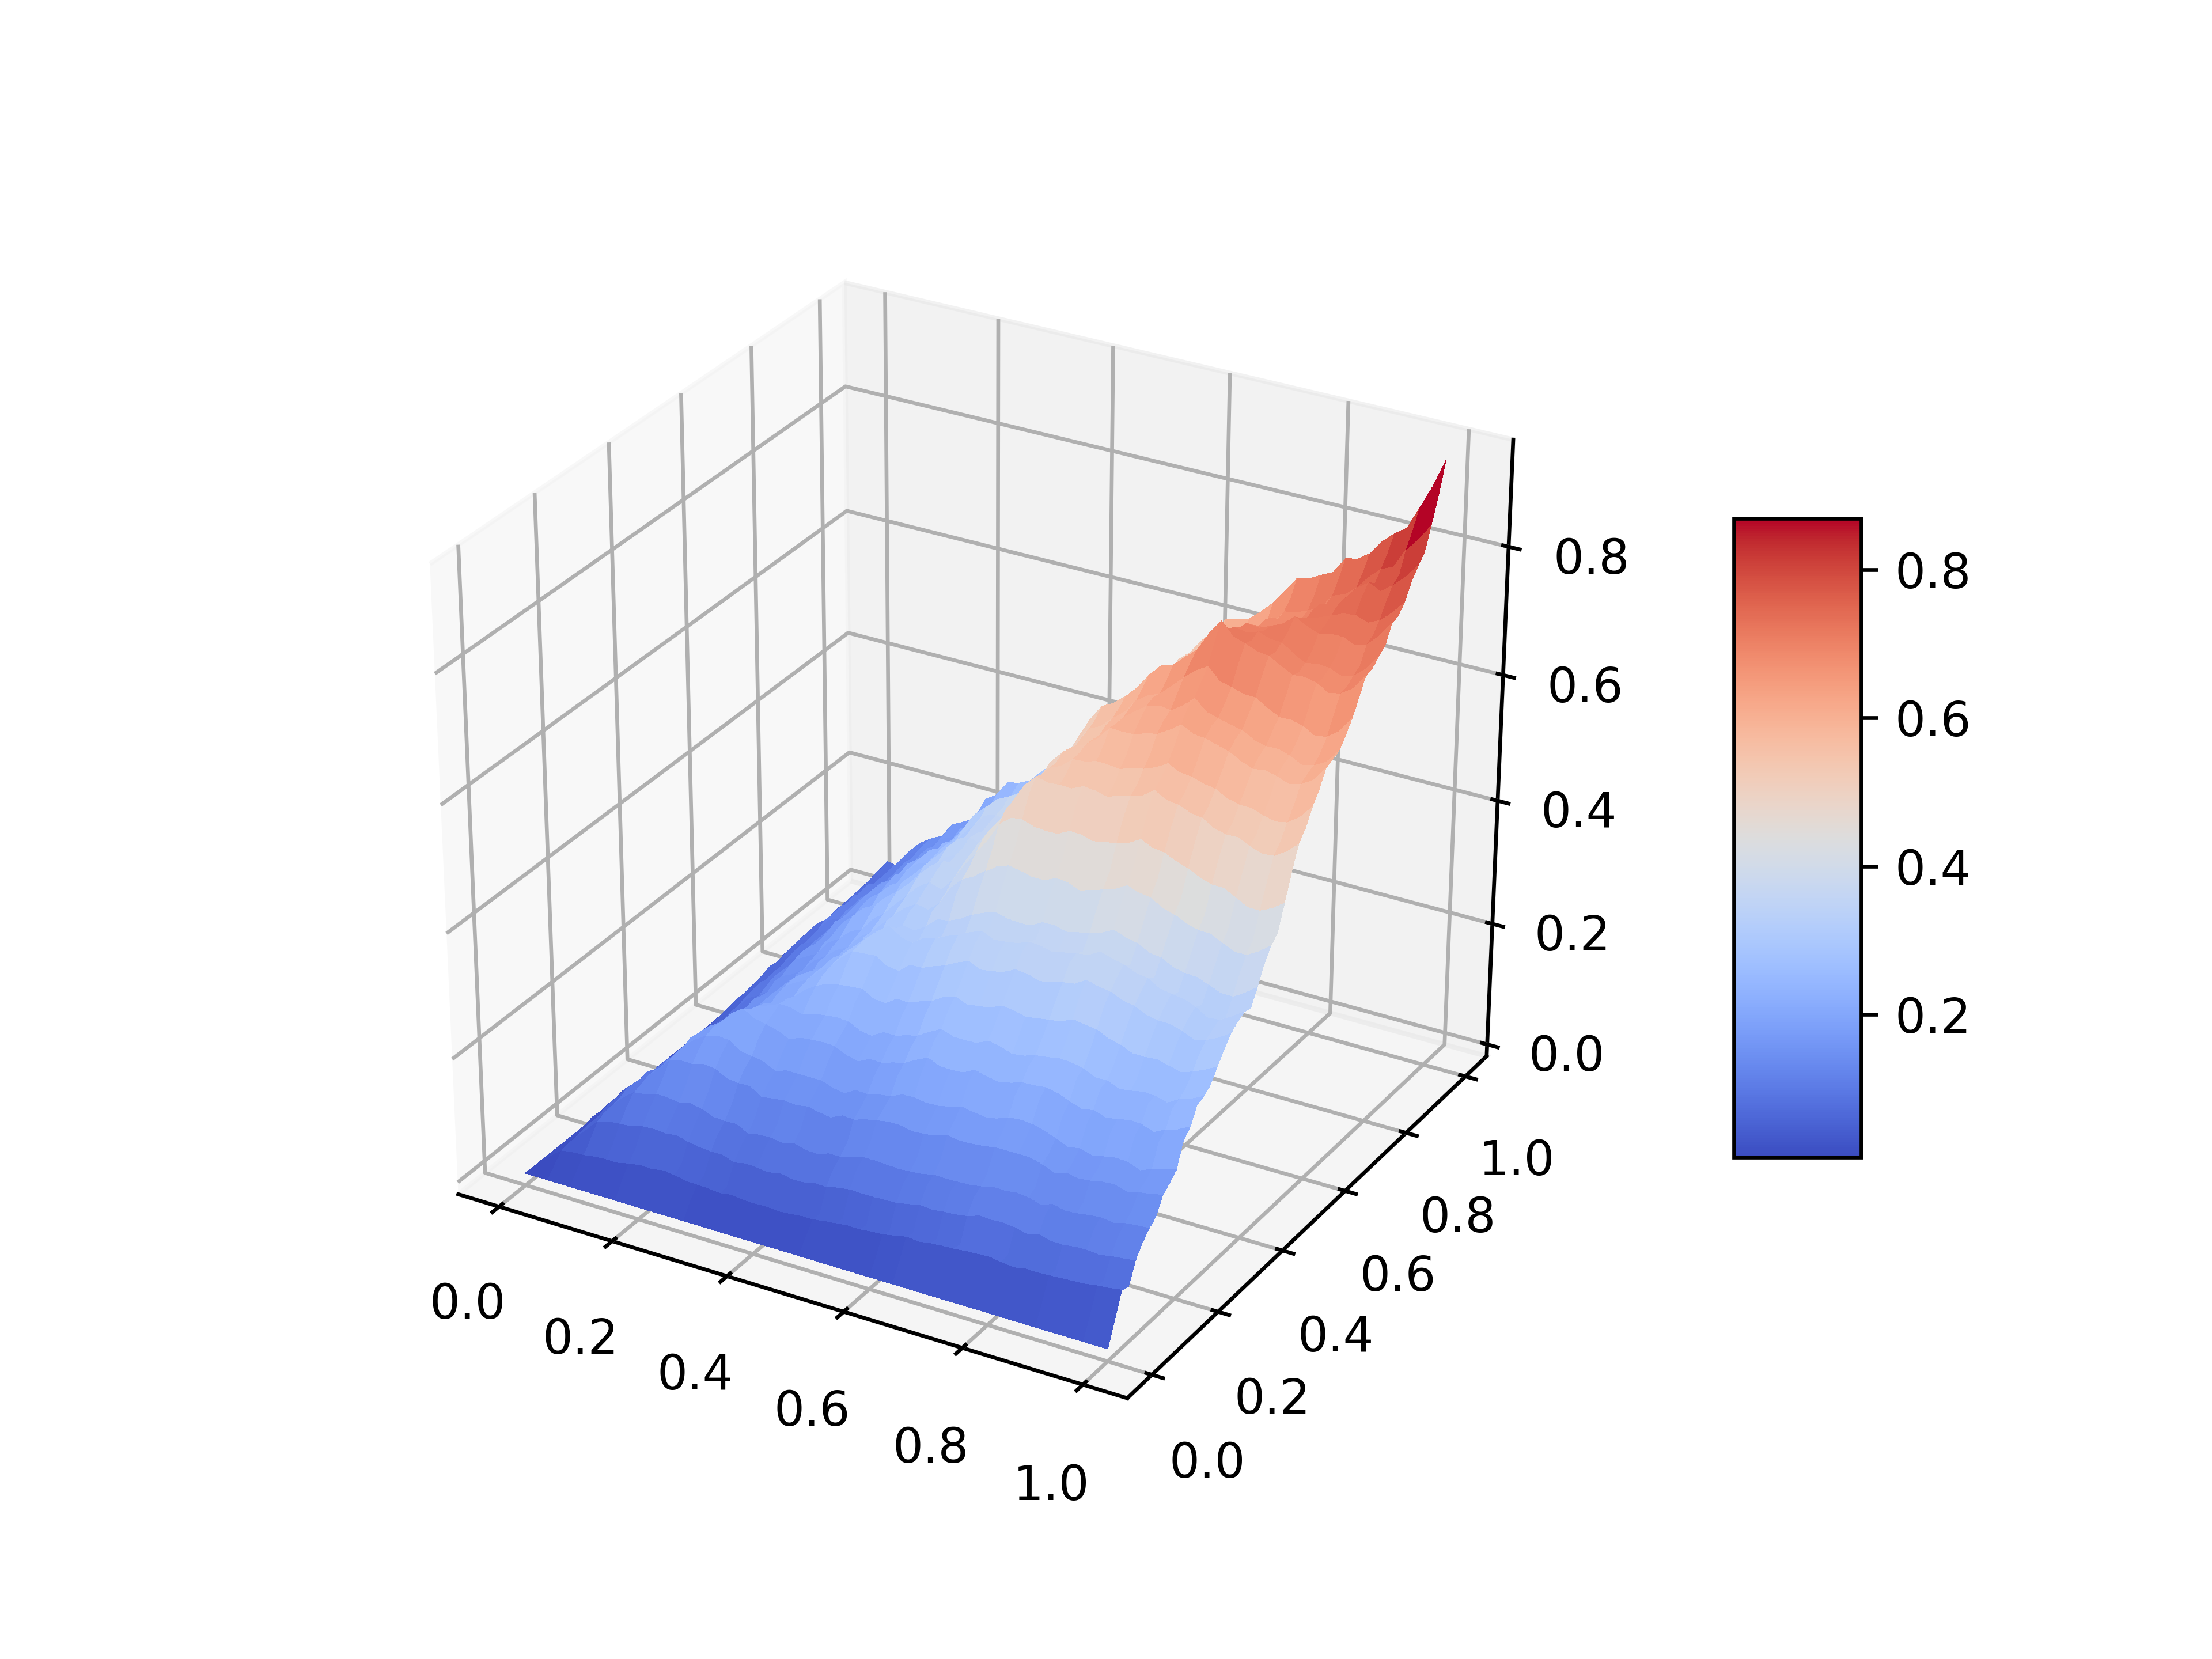
\includegraphics[scale=0.4]{covariance-1-55.png}
		\caption{H=0.55}
		\endminipage\hfill
		\minipage{0.49\textwidth}
		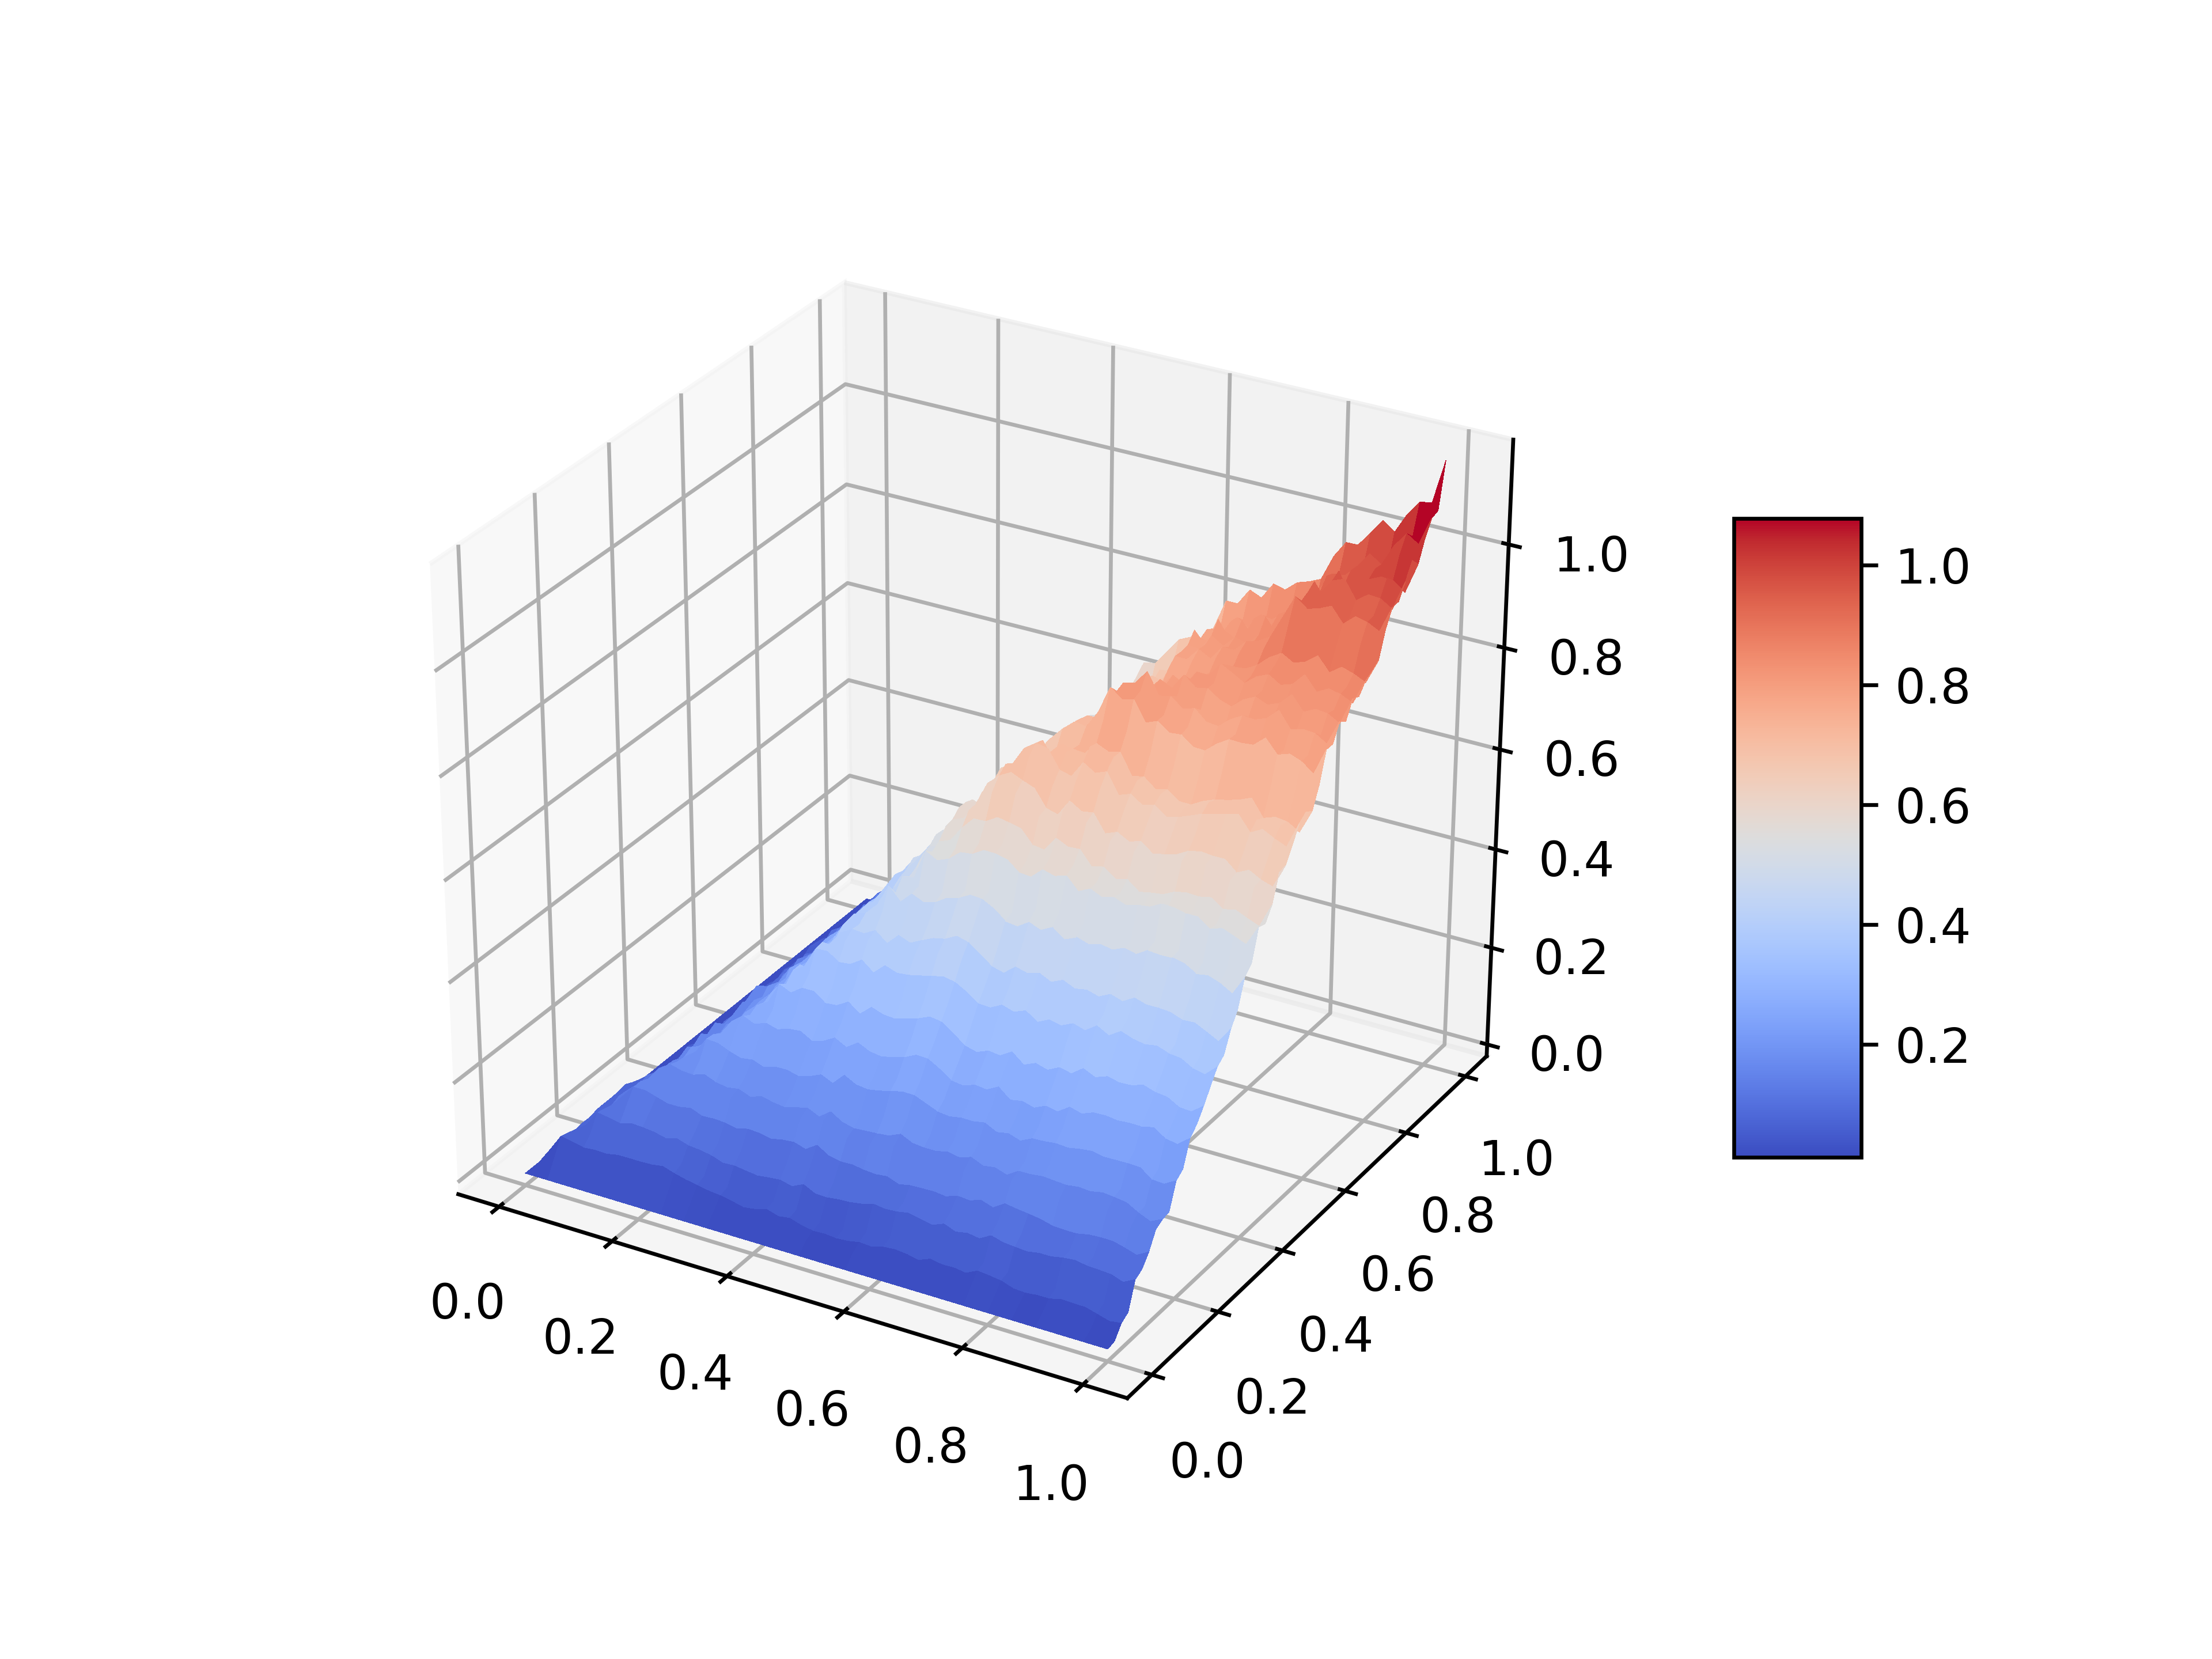
\includegraphics[scale=0.4]{covariance-1-45.png}
		\caption{H=0.45}
		\endminipage\hfill
	\end{figure}
	
	\begin{figure}[H]
		\minipage{0.49\textwidth}
		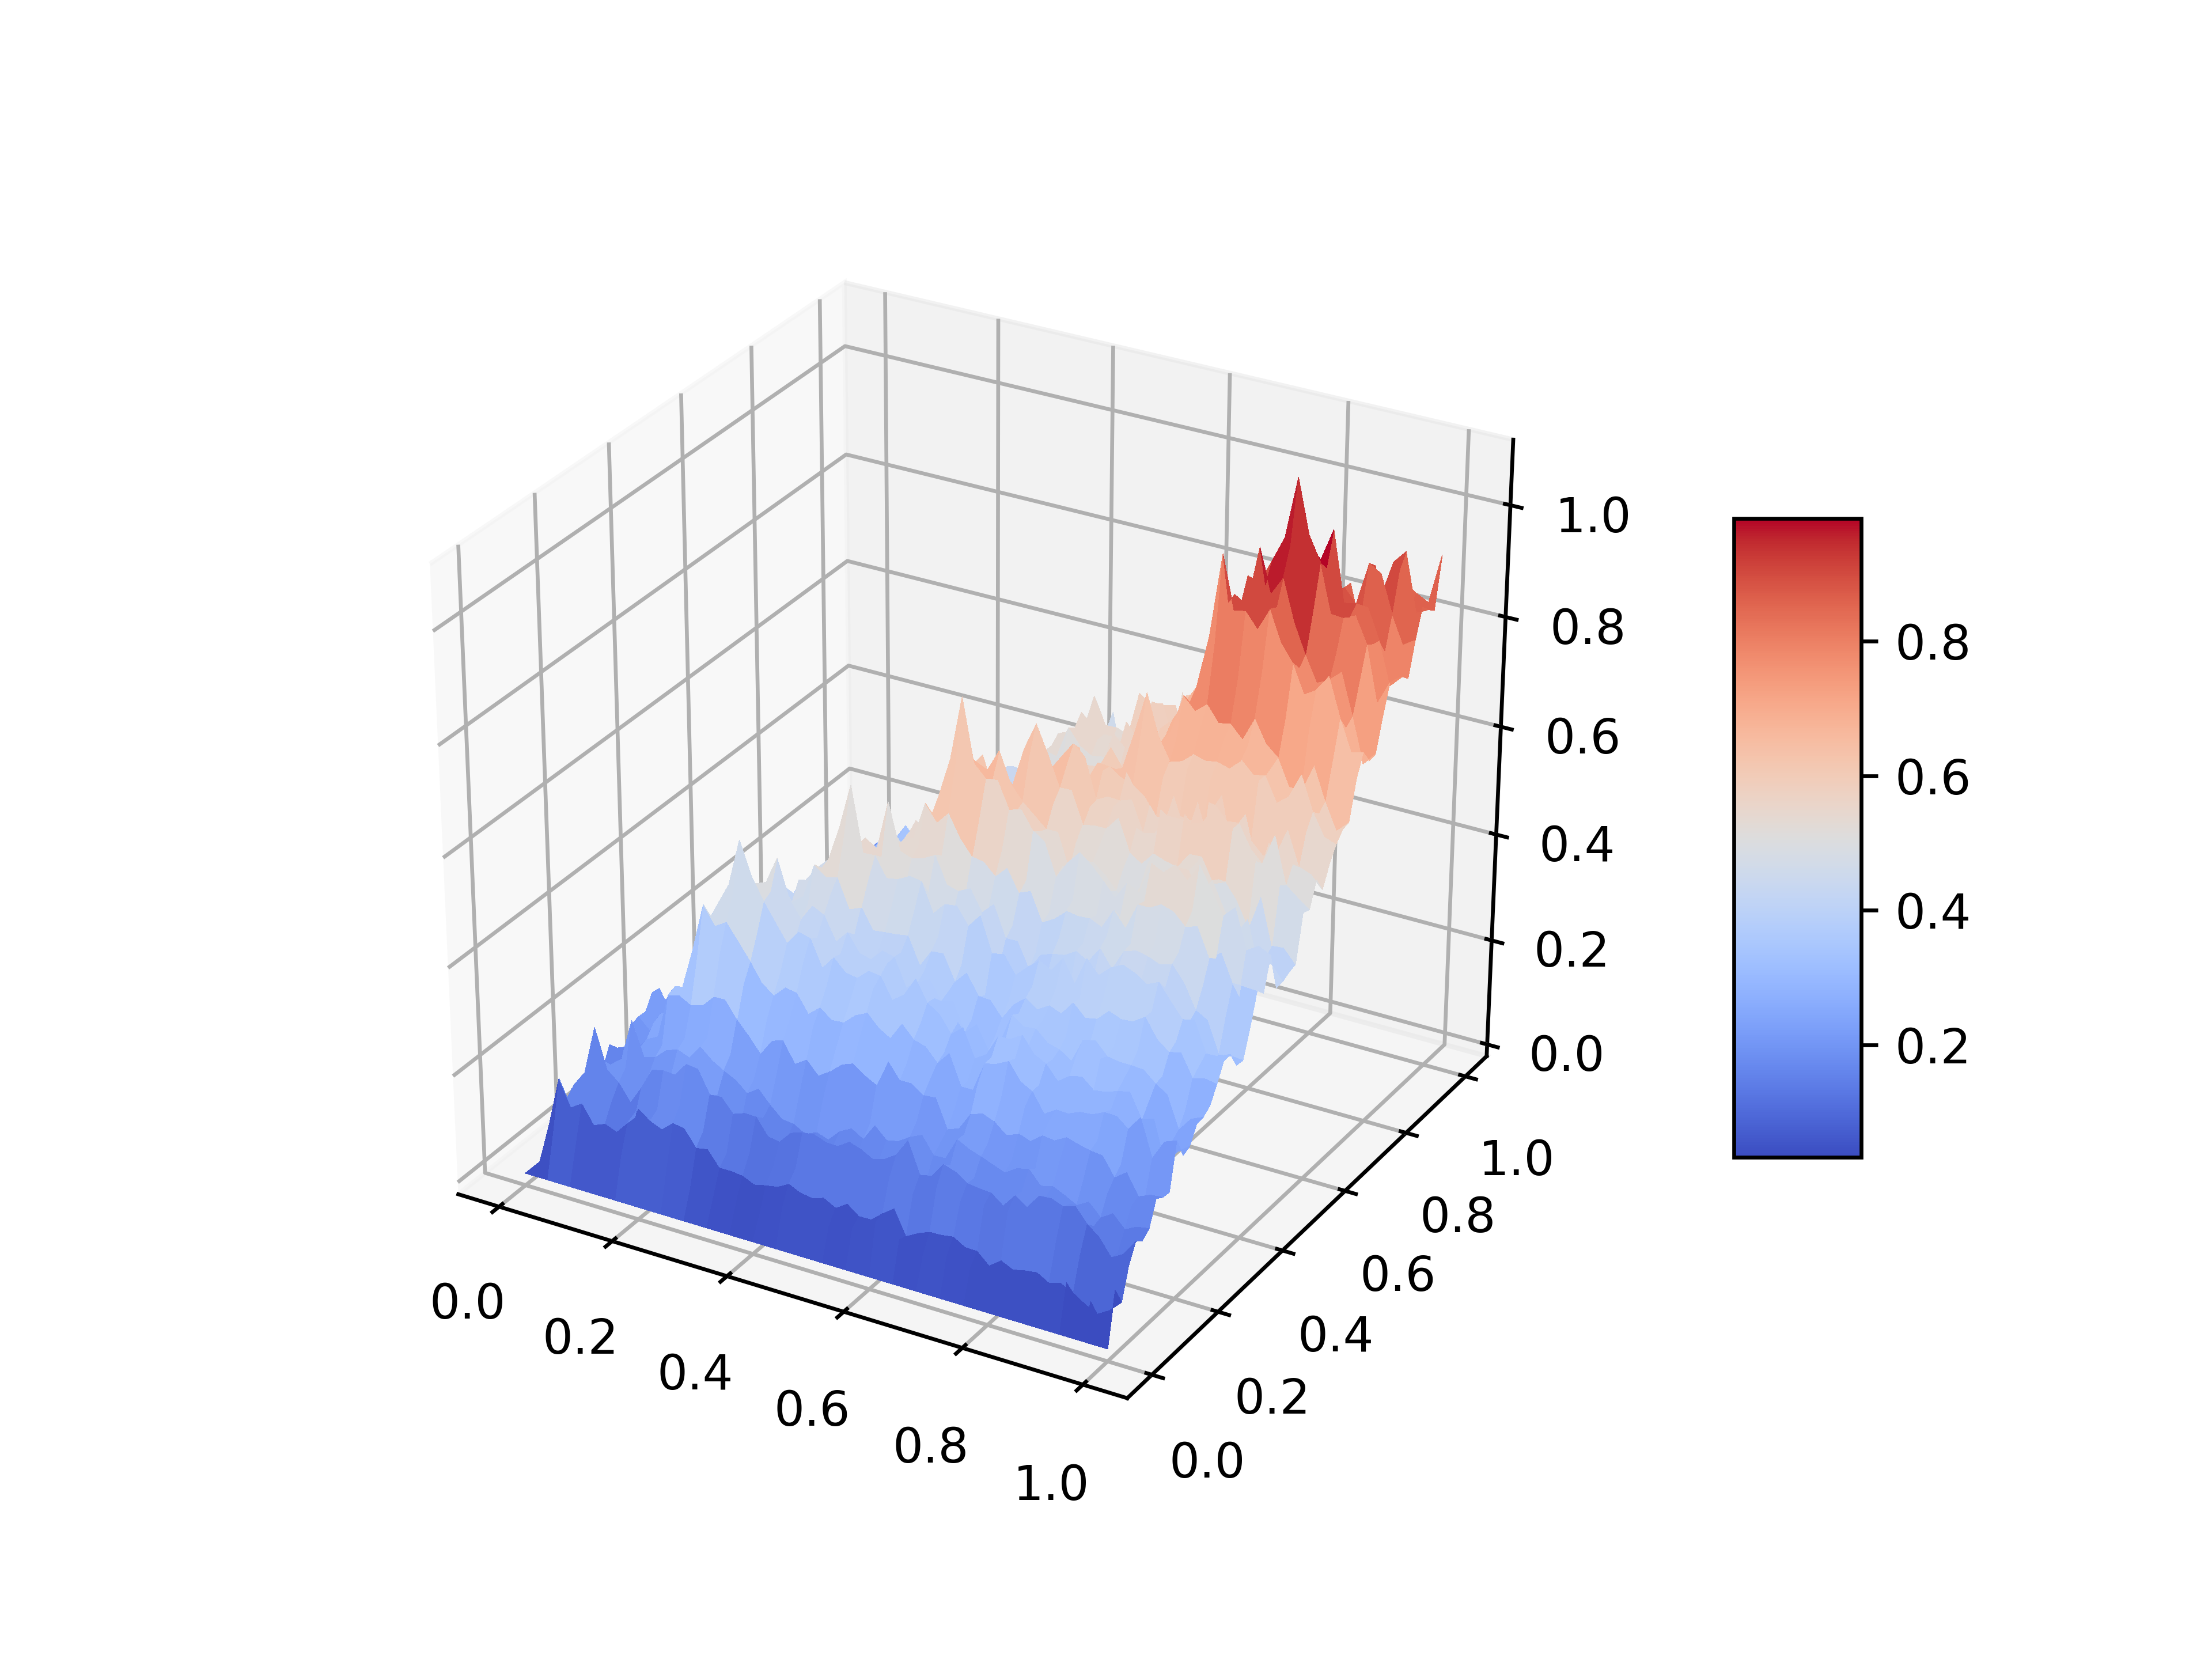
\includegraphics[scale=0.4]{covariance-1-25.png}
		\caption{H=0.25}
		\endminipage\hfill
		\minipage{0.49\textwidth}
		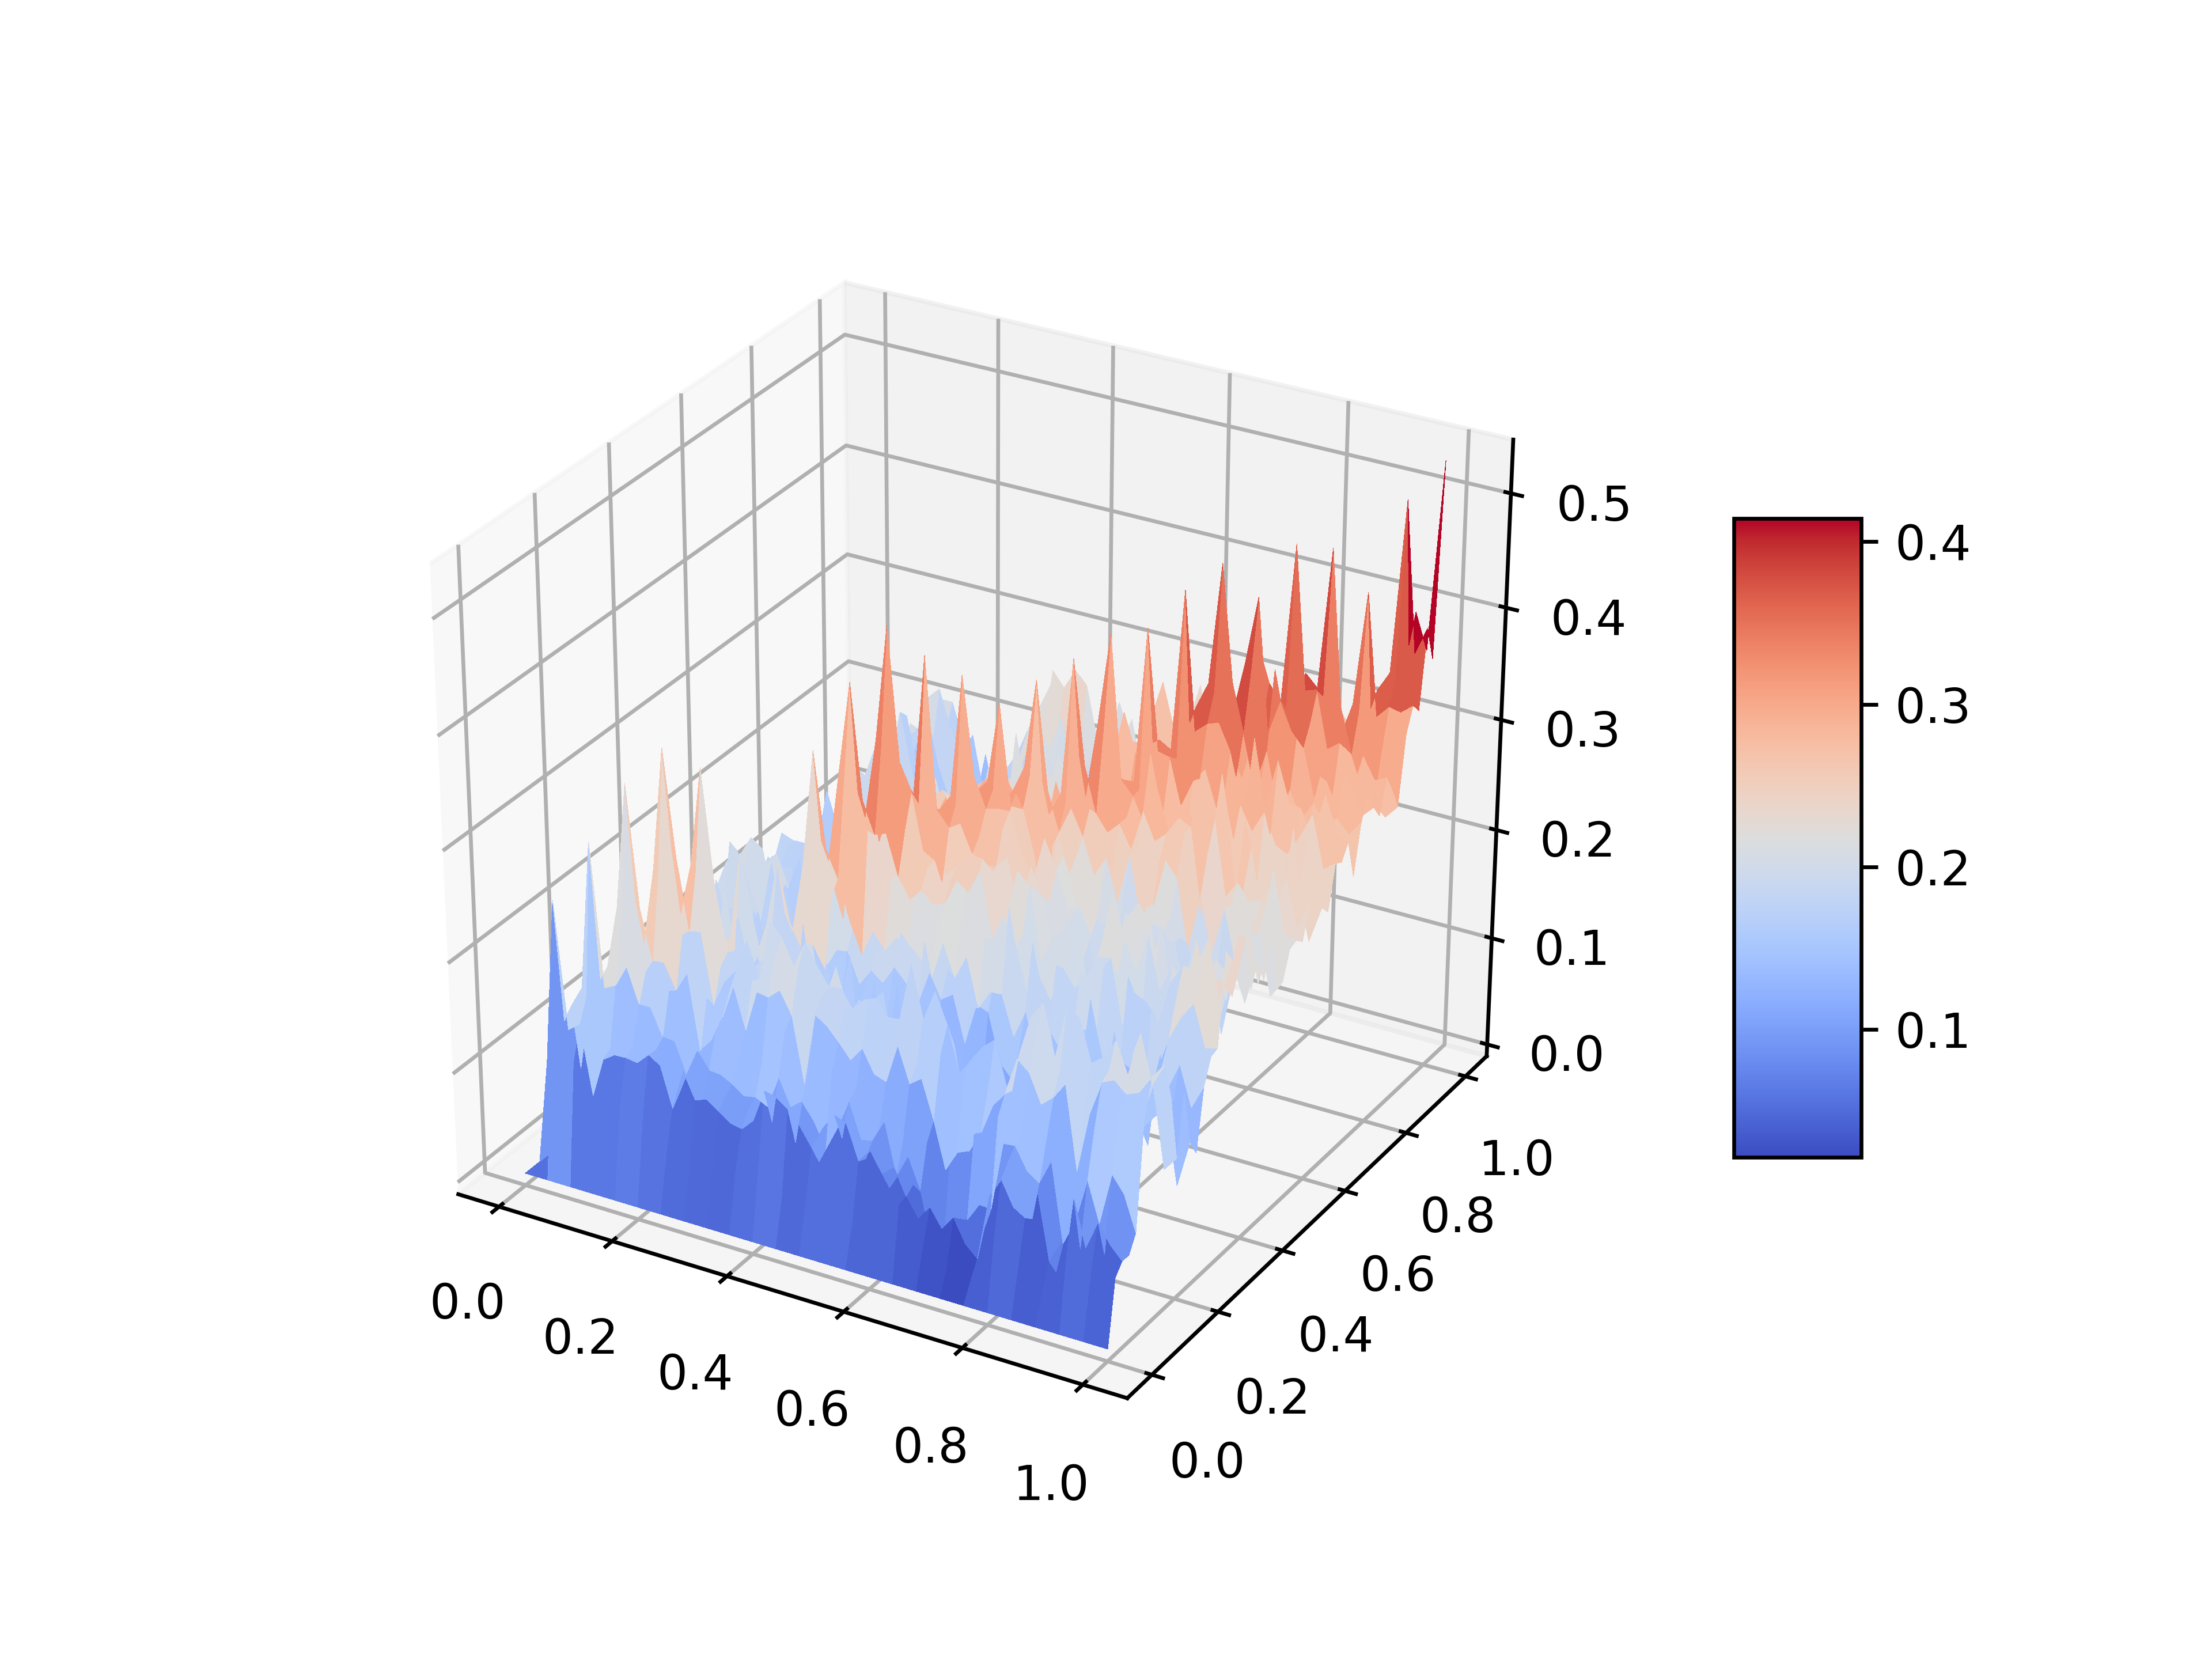
\includegraphics[scale=0.4]{covariance-1-05.png}
		\caption{H=0.05}
		\endminipage\hfill
	\end{figure}
	
	Кроме того можно вычислить выборочное среднее:
	\begin{figure}[H]
		\minipage{0.49\textwidth}
		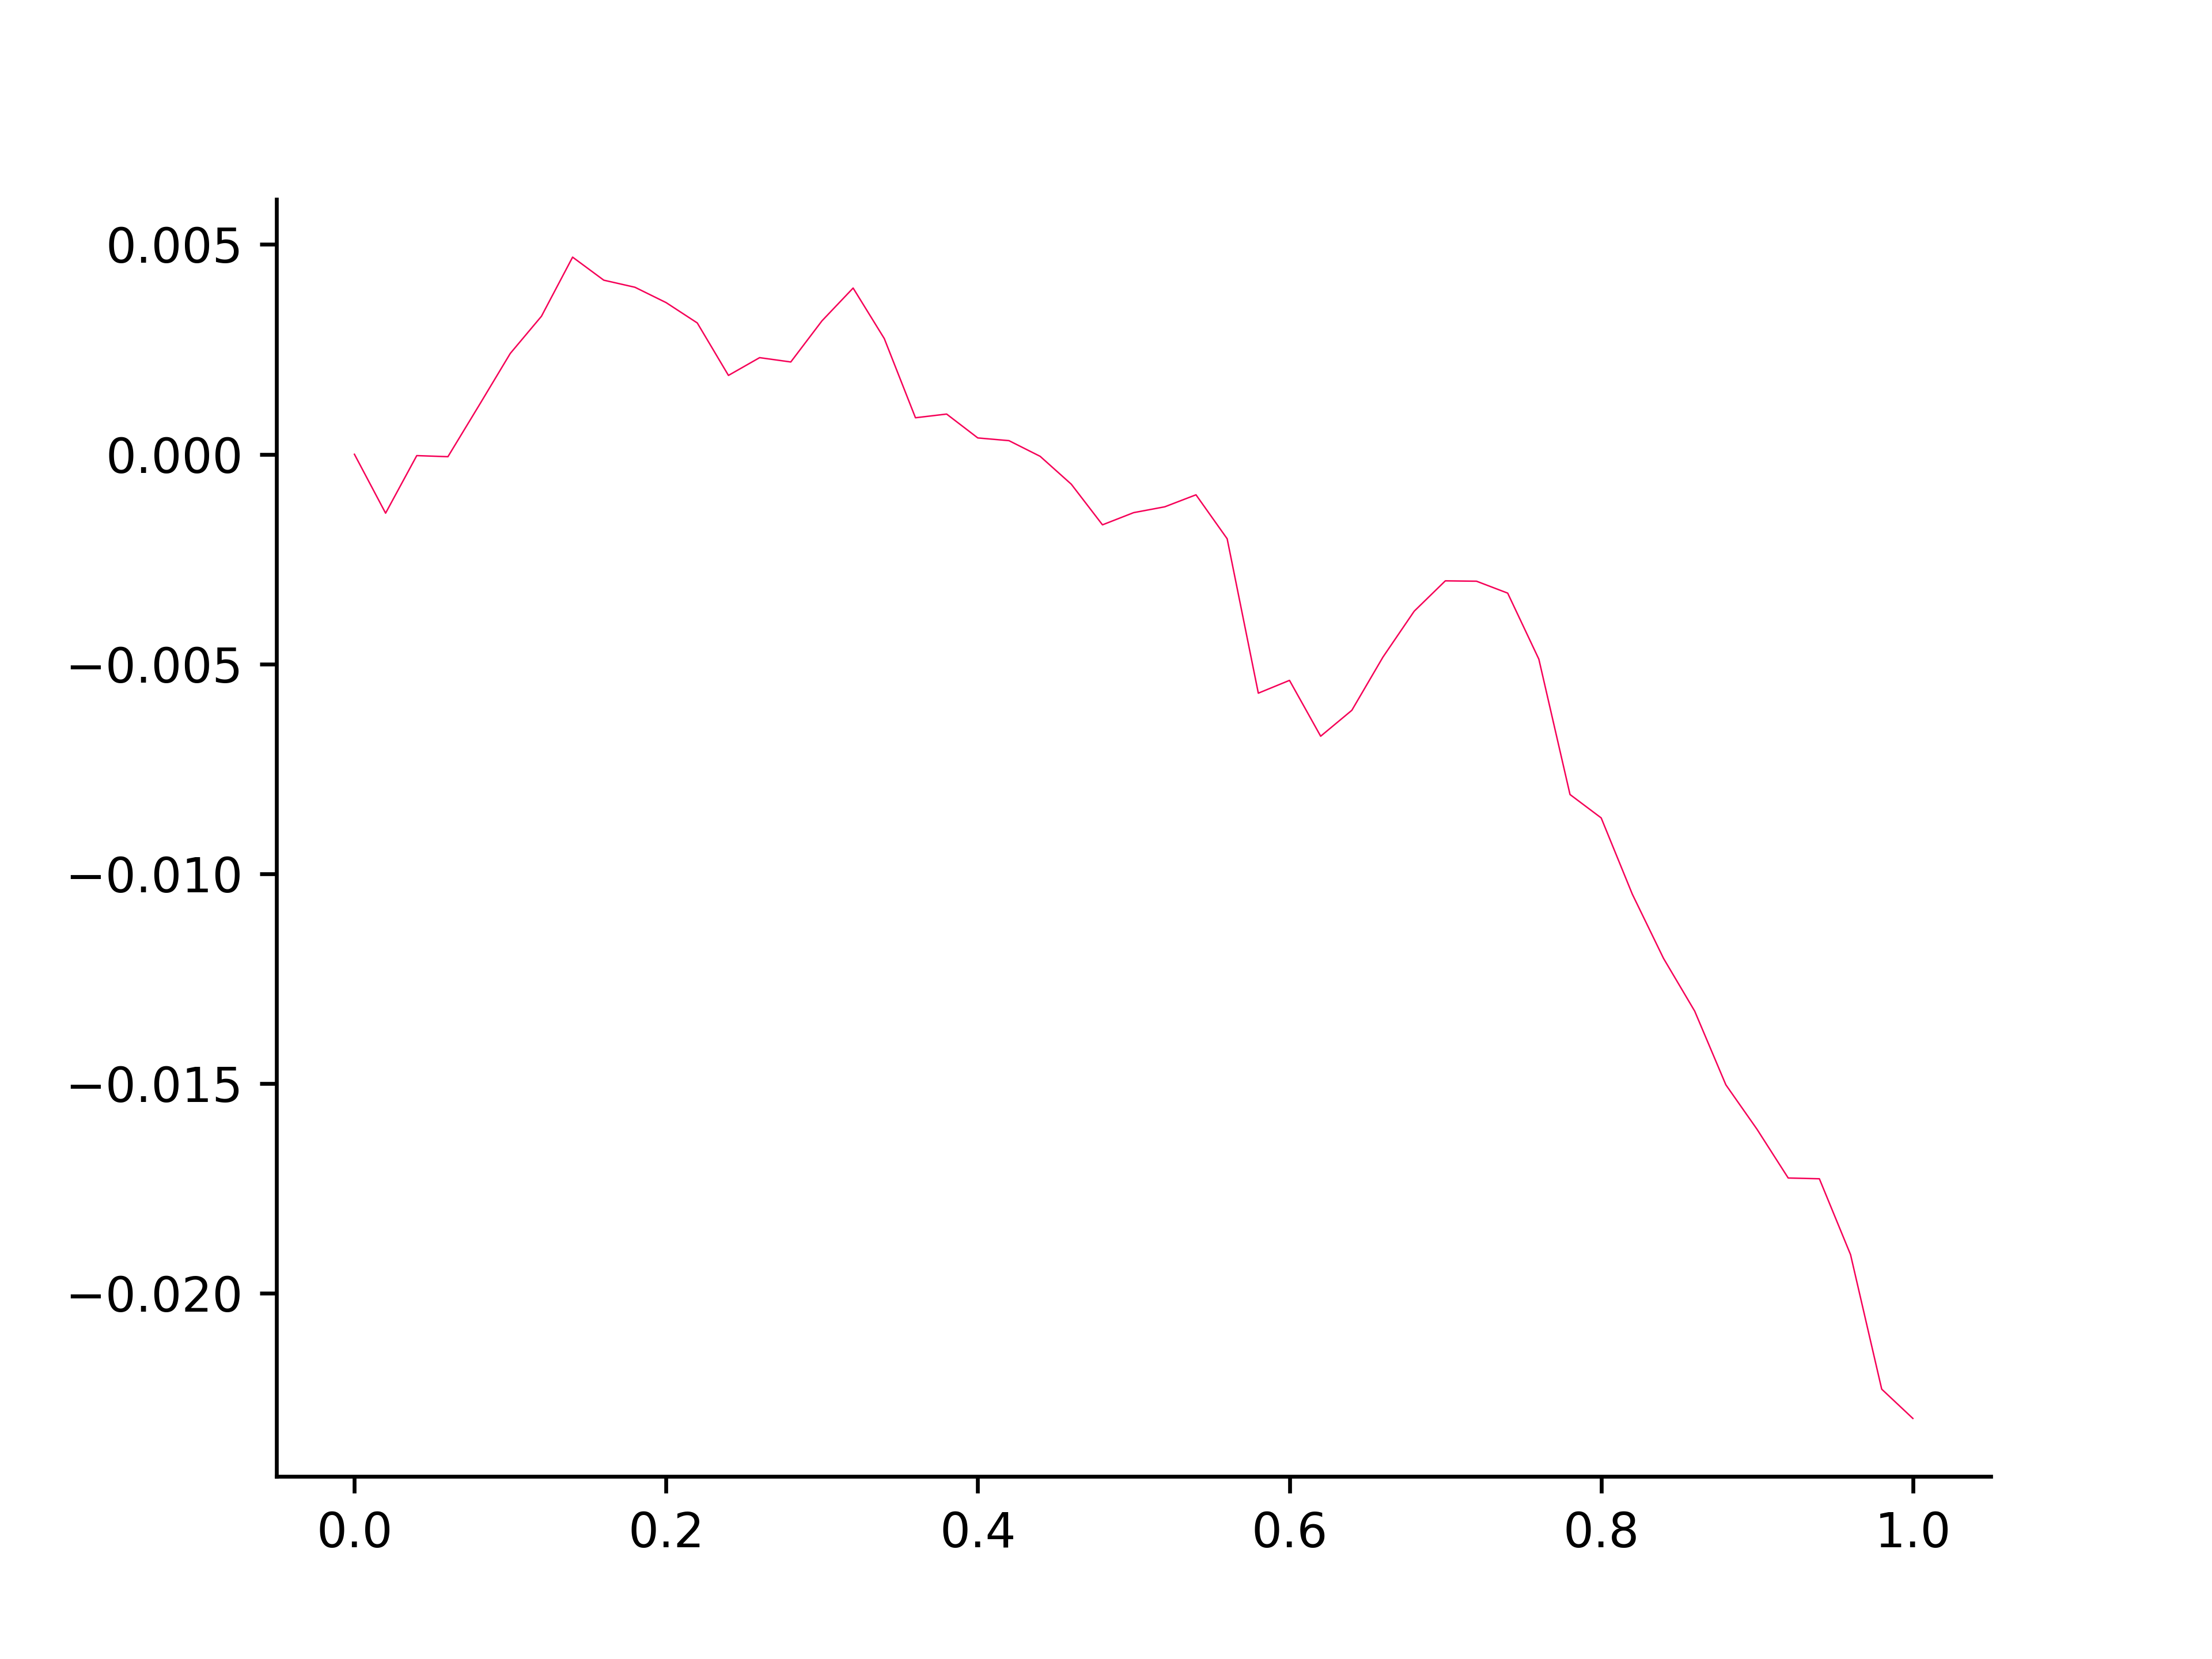
\includegraphics[scale=0.4]{mean-1-95.png}
		\caption{H=0.95}
		\endminipage\hfill
		\minipage{0.49\textwidth}
		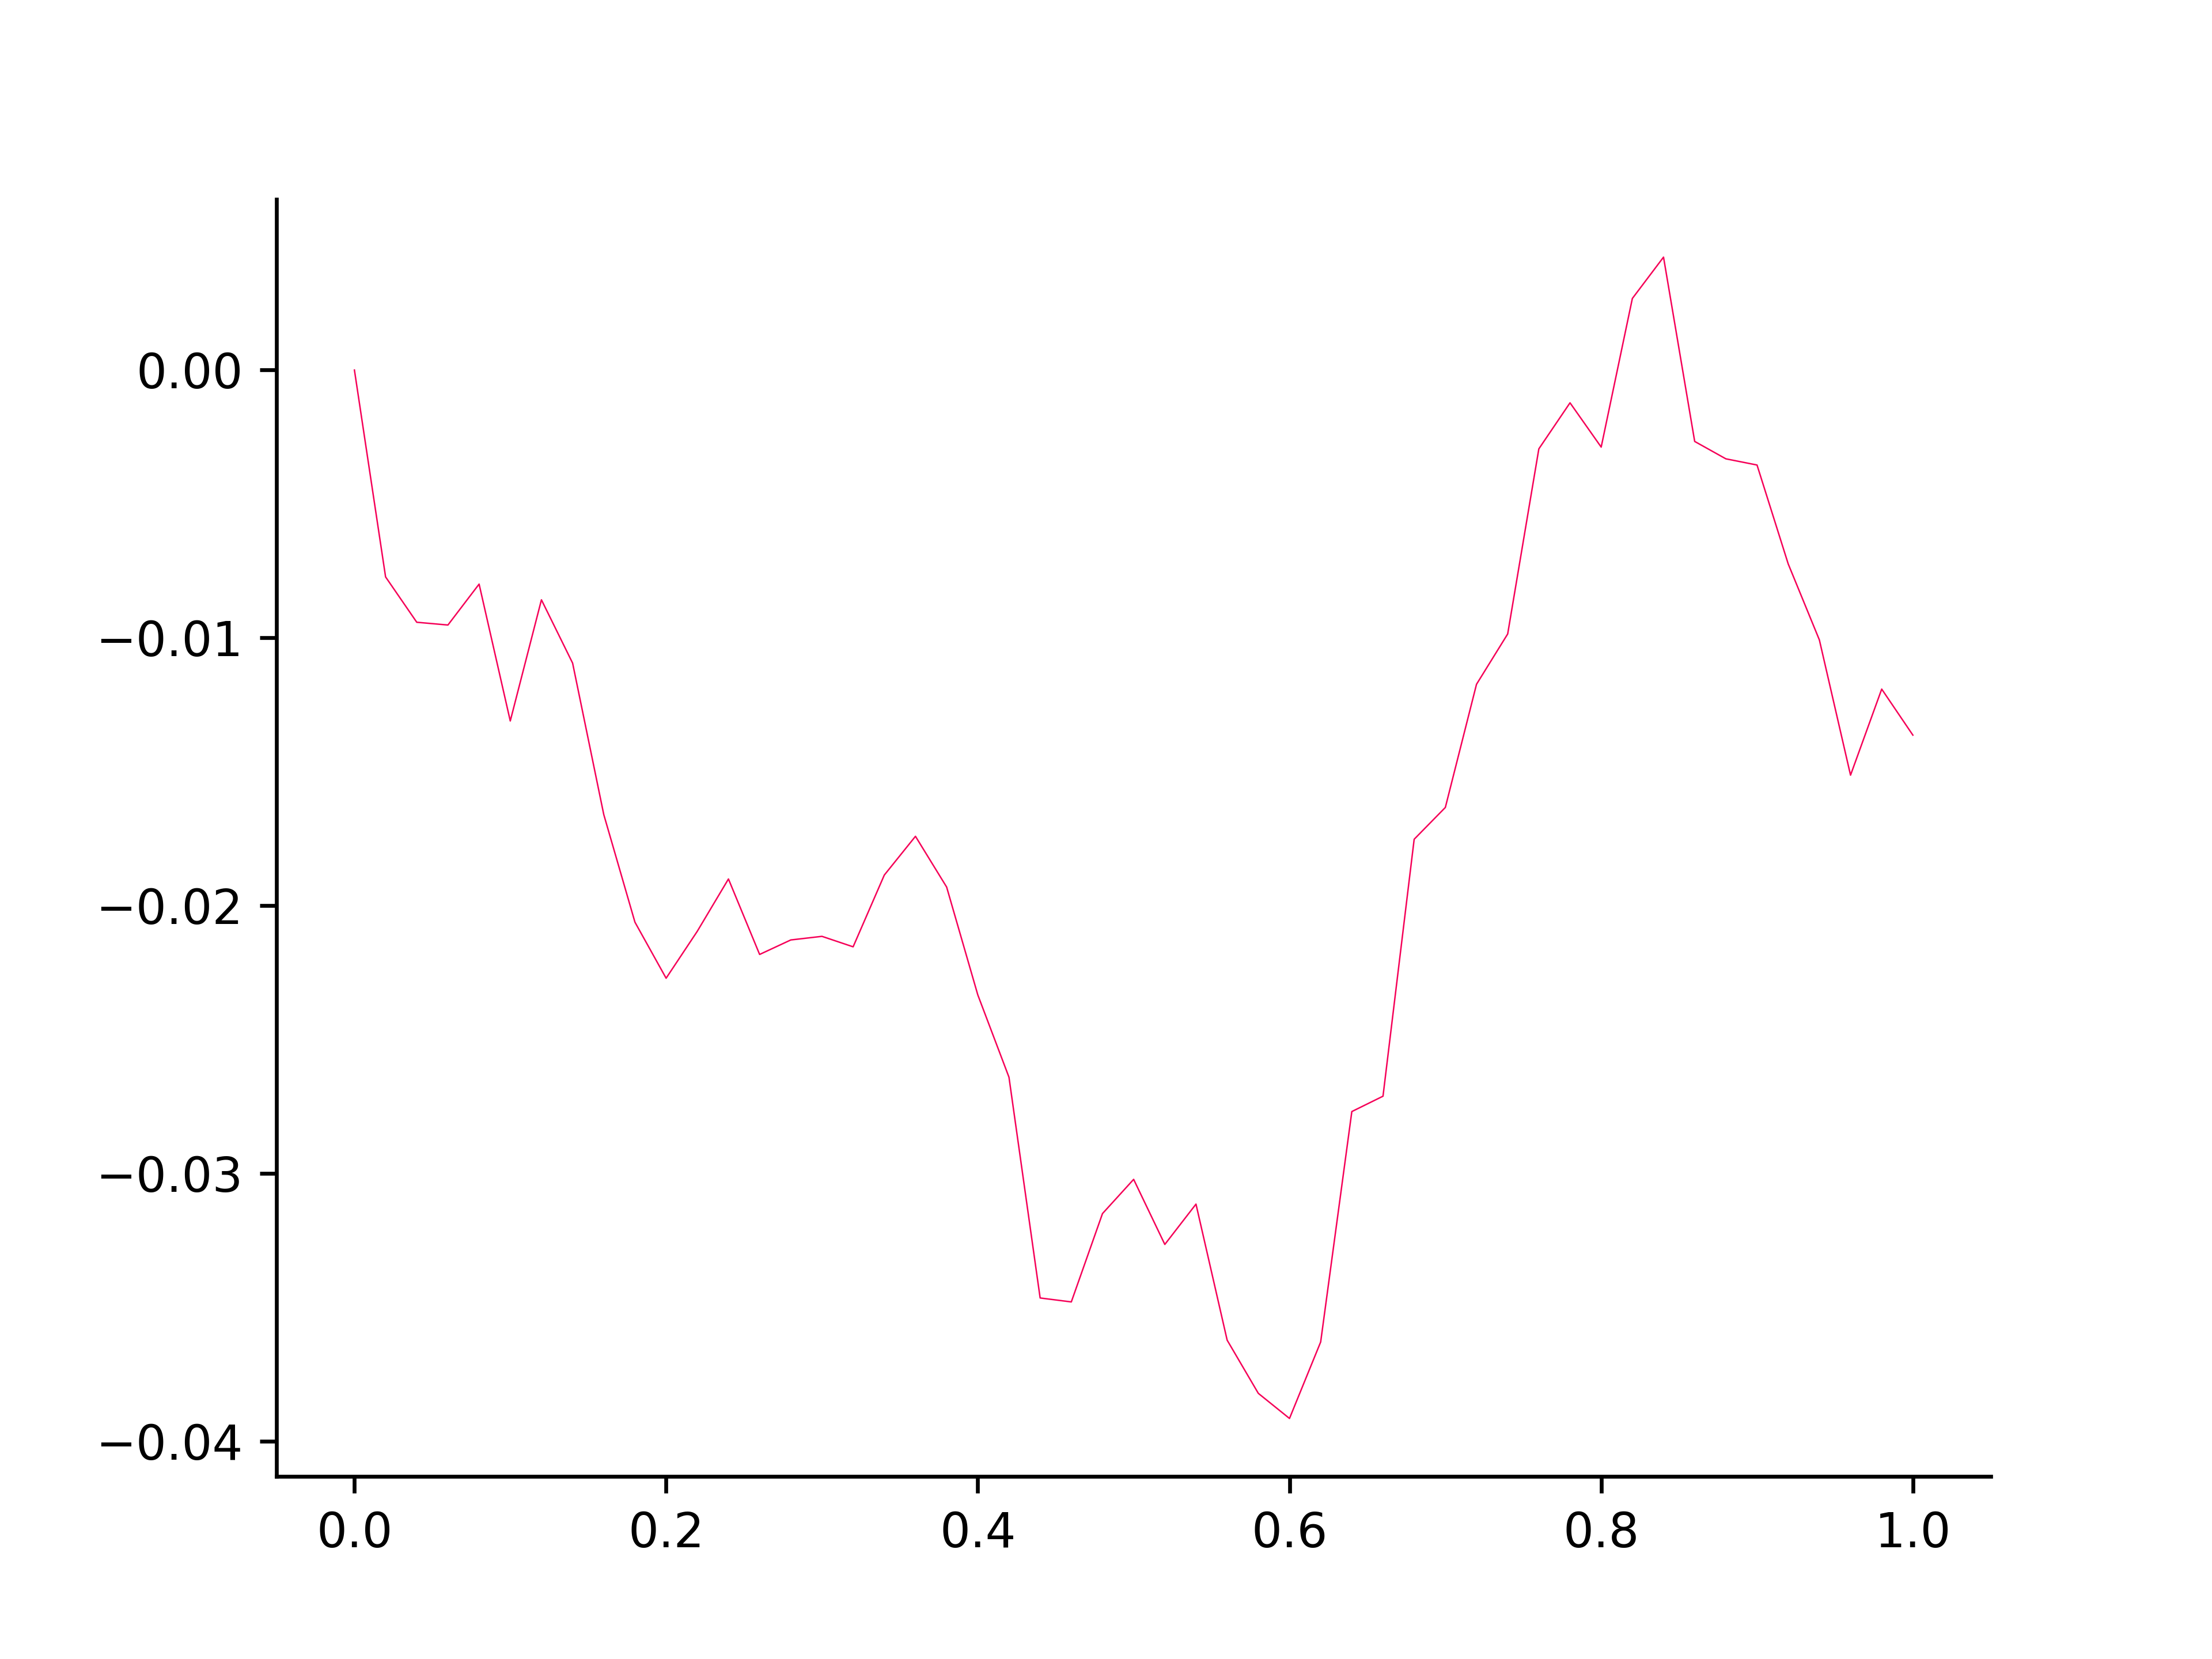
\includegraphics[scale=0.4]{mean-1-75.png}
		\caption{H=0.75}
		\endminipage\hfill
	\end{figure}
	
	\begin{figure}[H]
		\minipage{0.49\textwidth}
		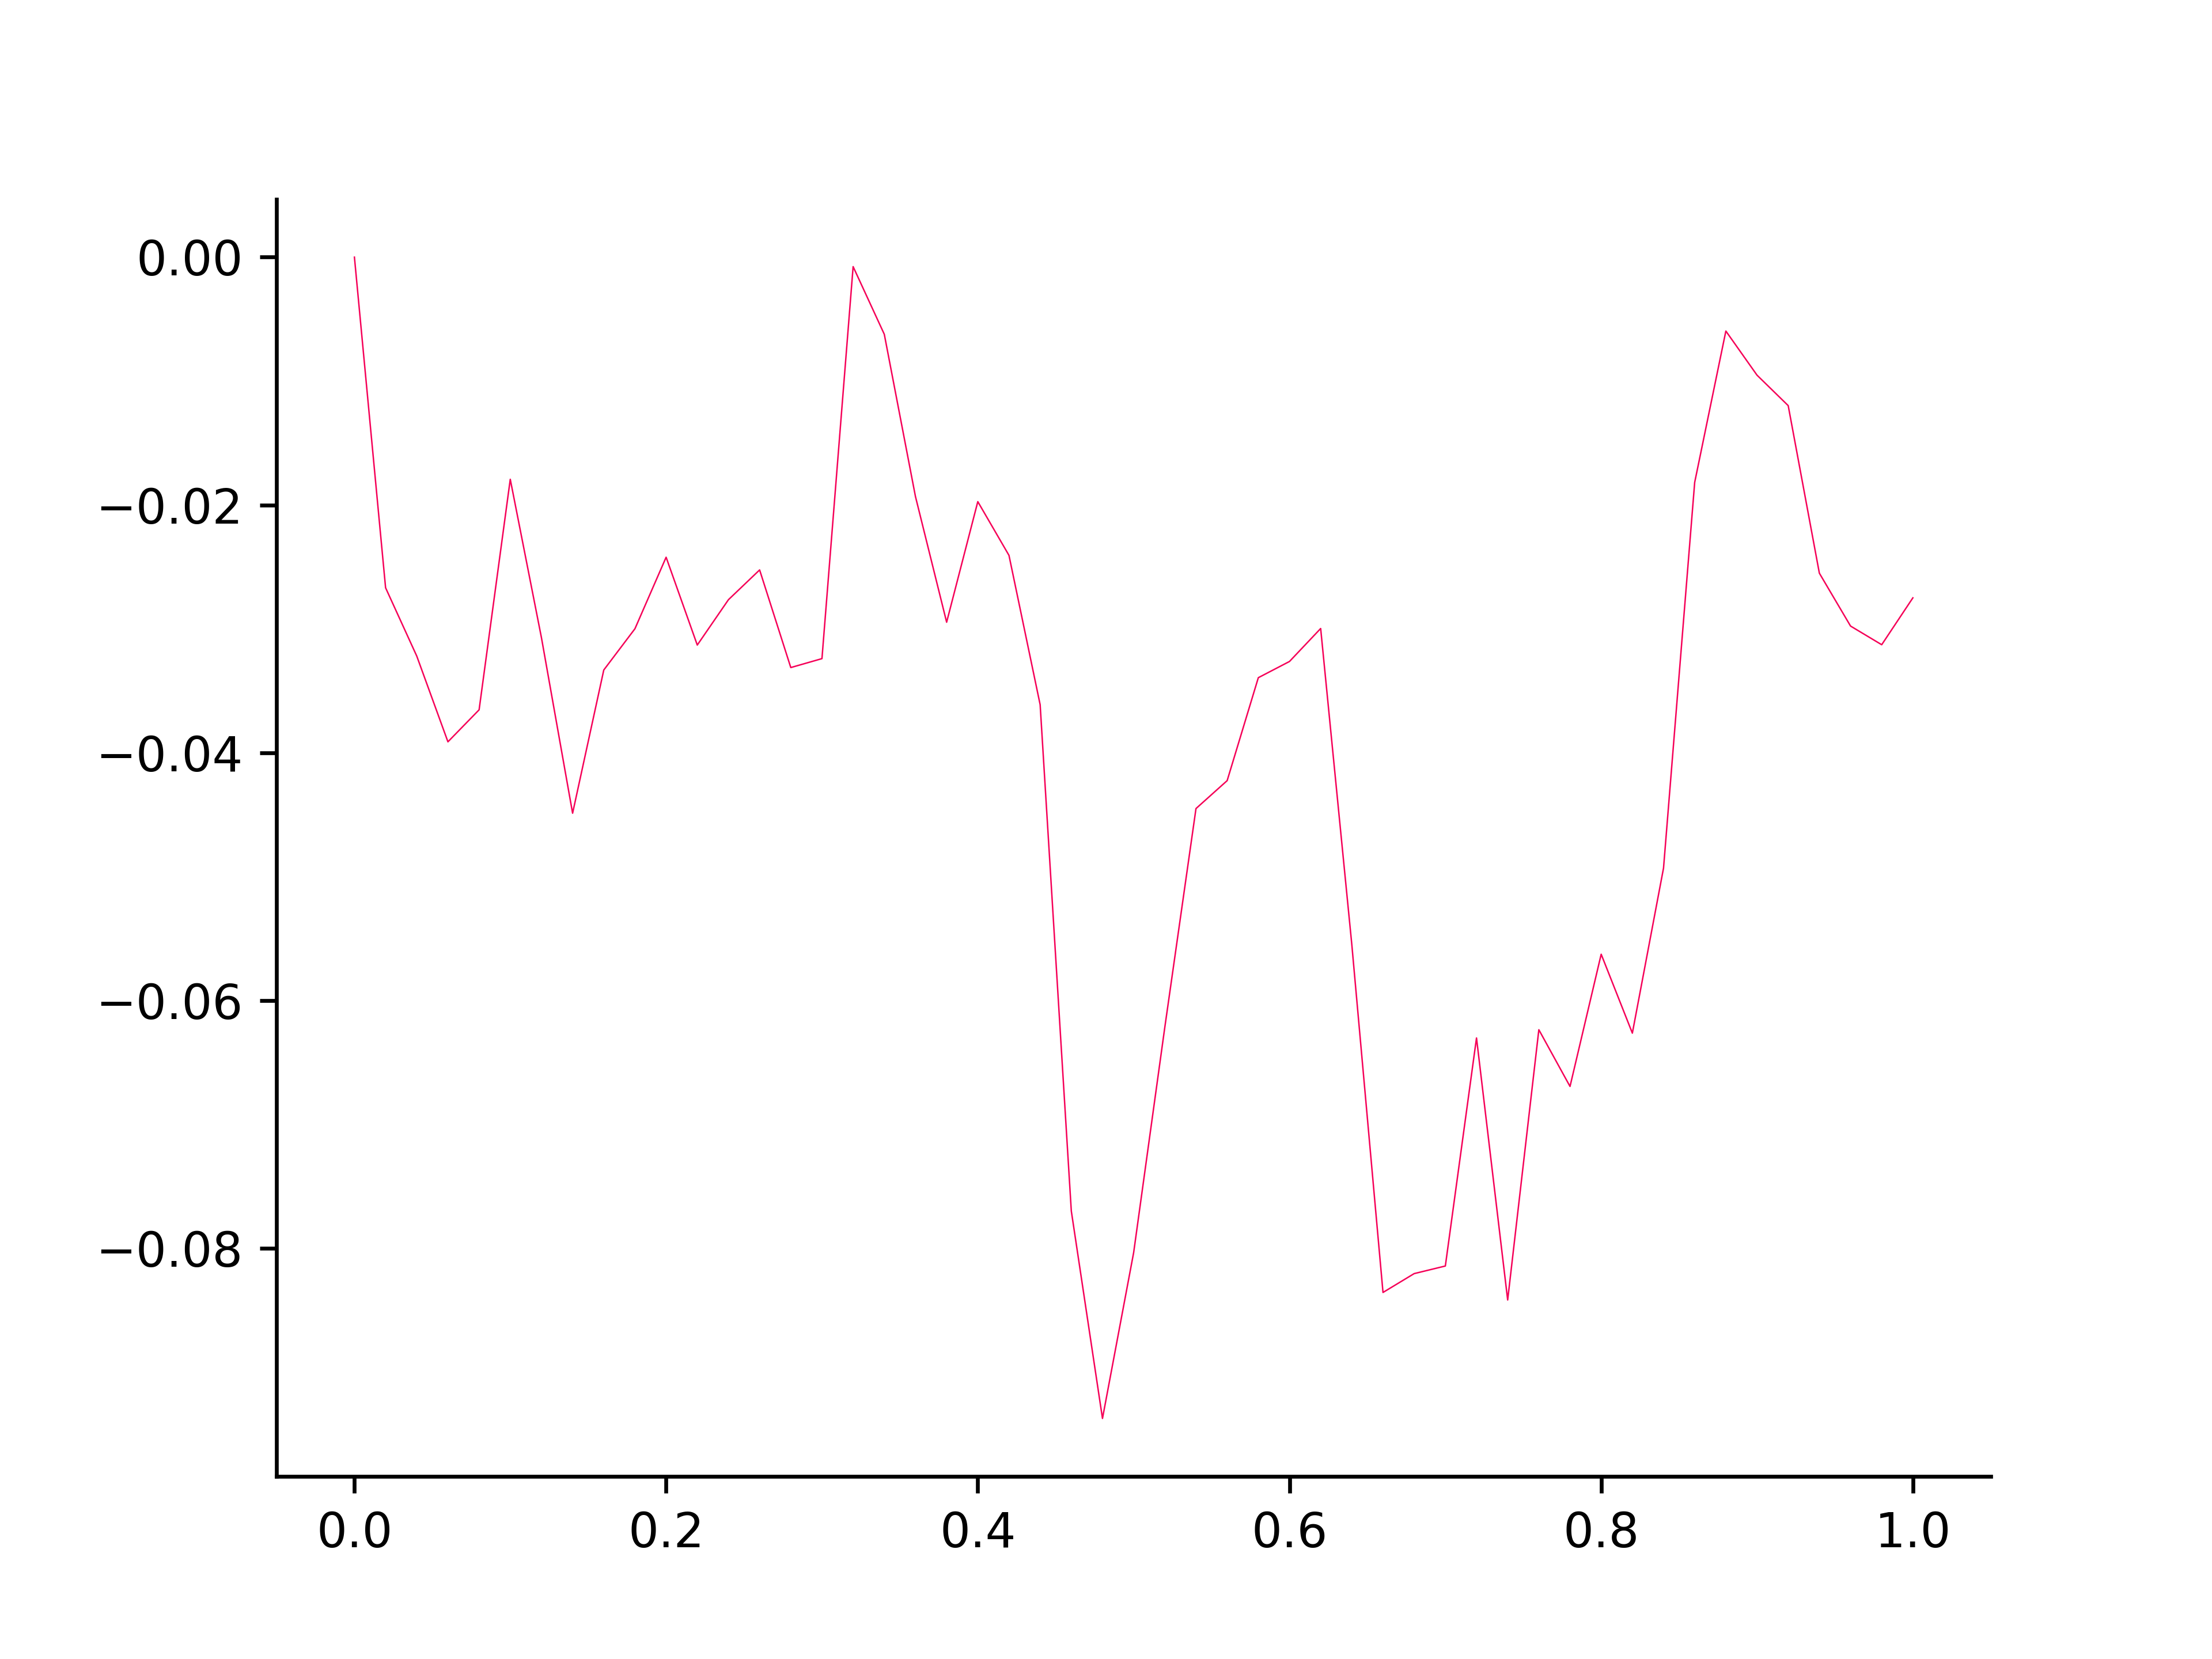
\includegraphics[scale=0.4]{mean-1-55.png}
		\caption{H=0.55}
		\endminipage\hfill
		\minipage{0.49\textwidth}
		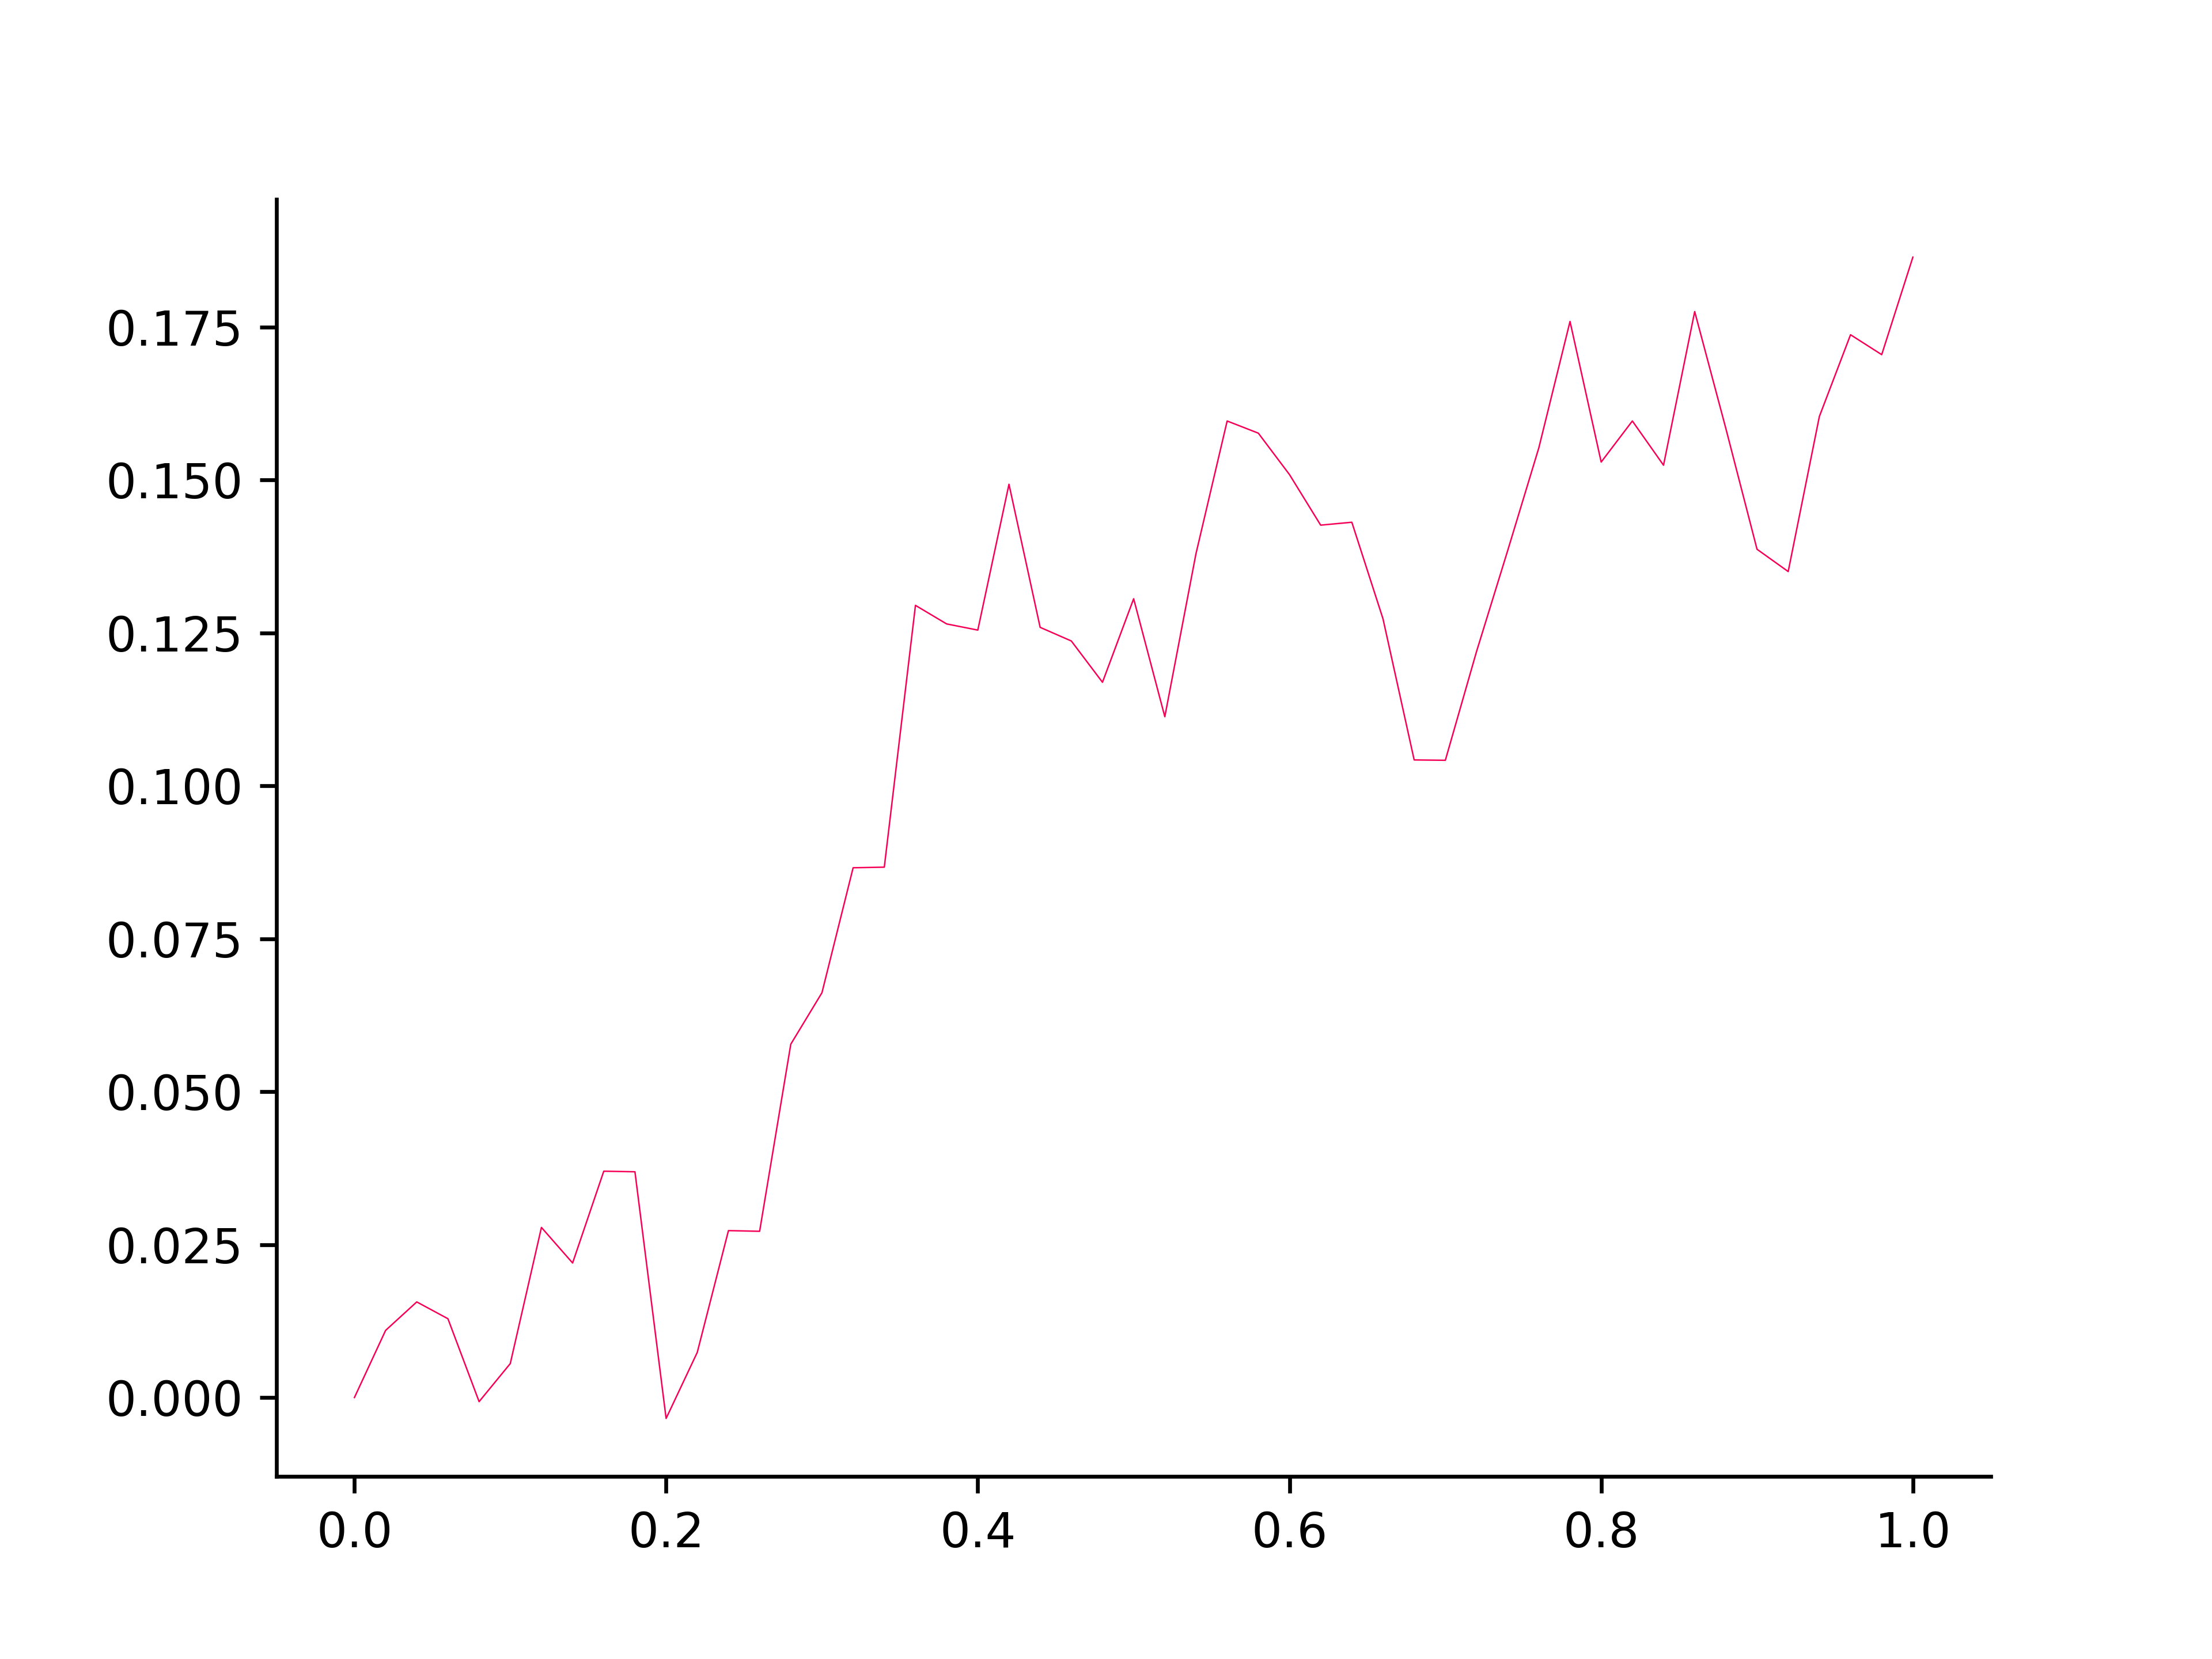
\includegraphics[scale=0.4]{mean-1-45.png}
		\caption{H=0.45}
		\endminipage\hfill
	\end{figure}
	
	\begin{figure}[H]
		\minipage{0.49\textwidth}
		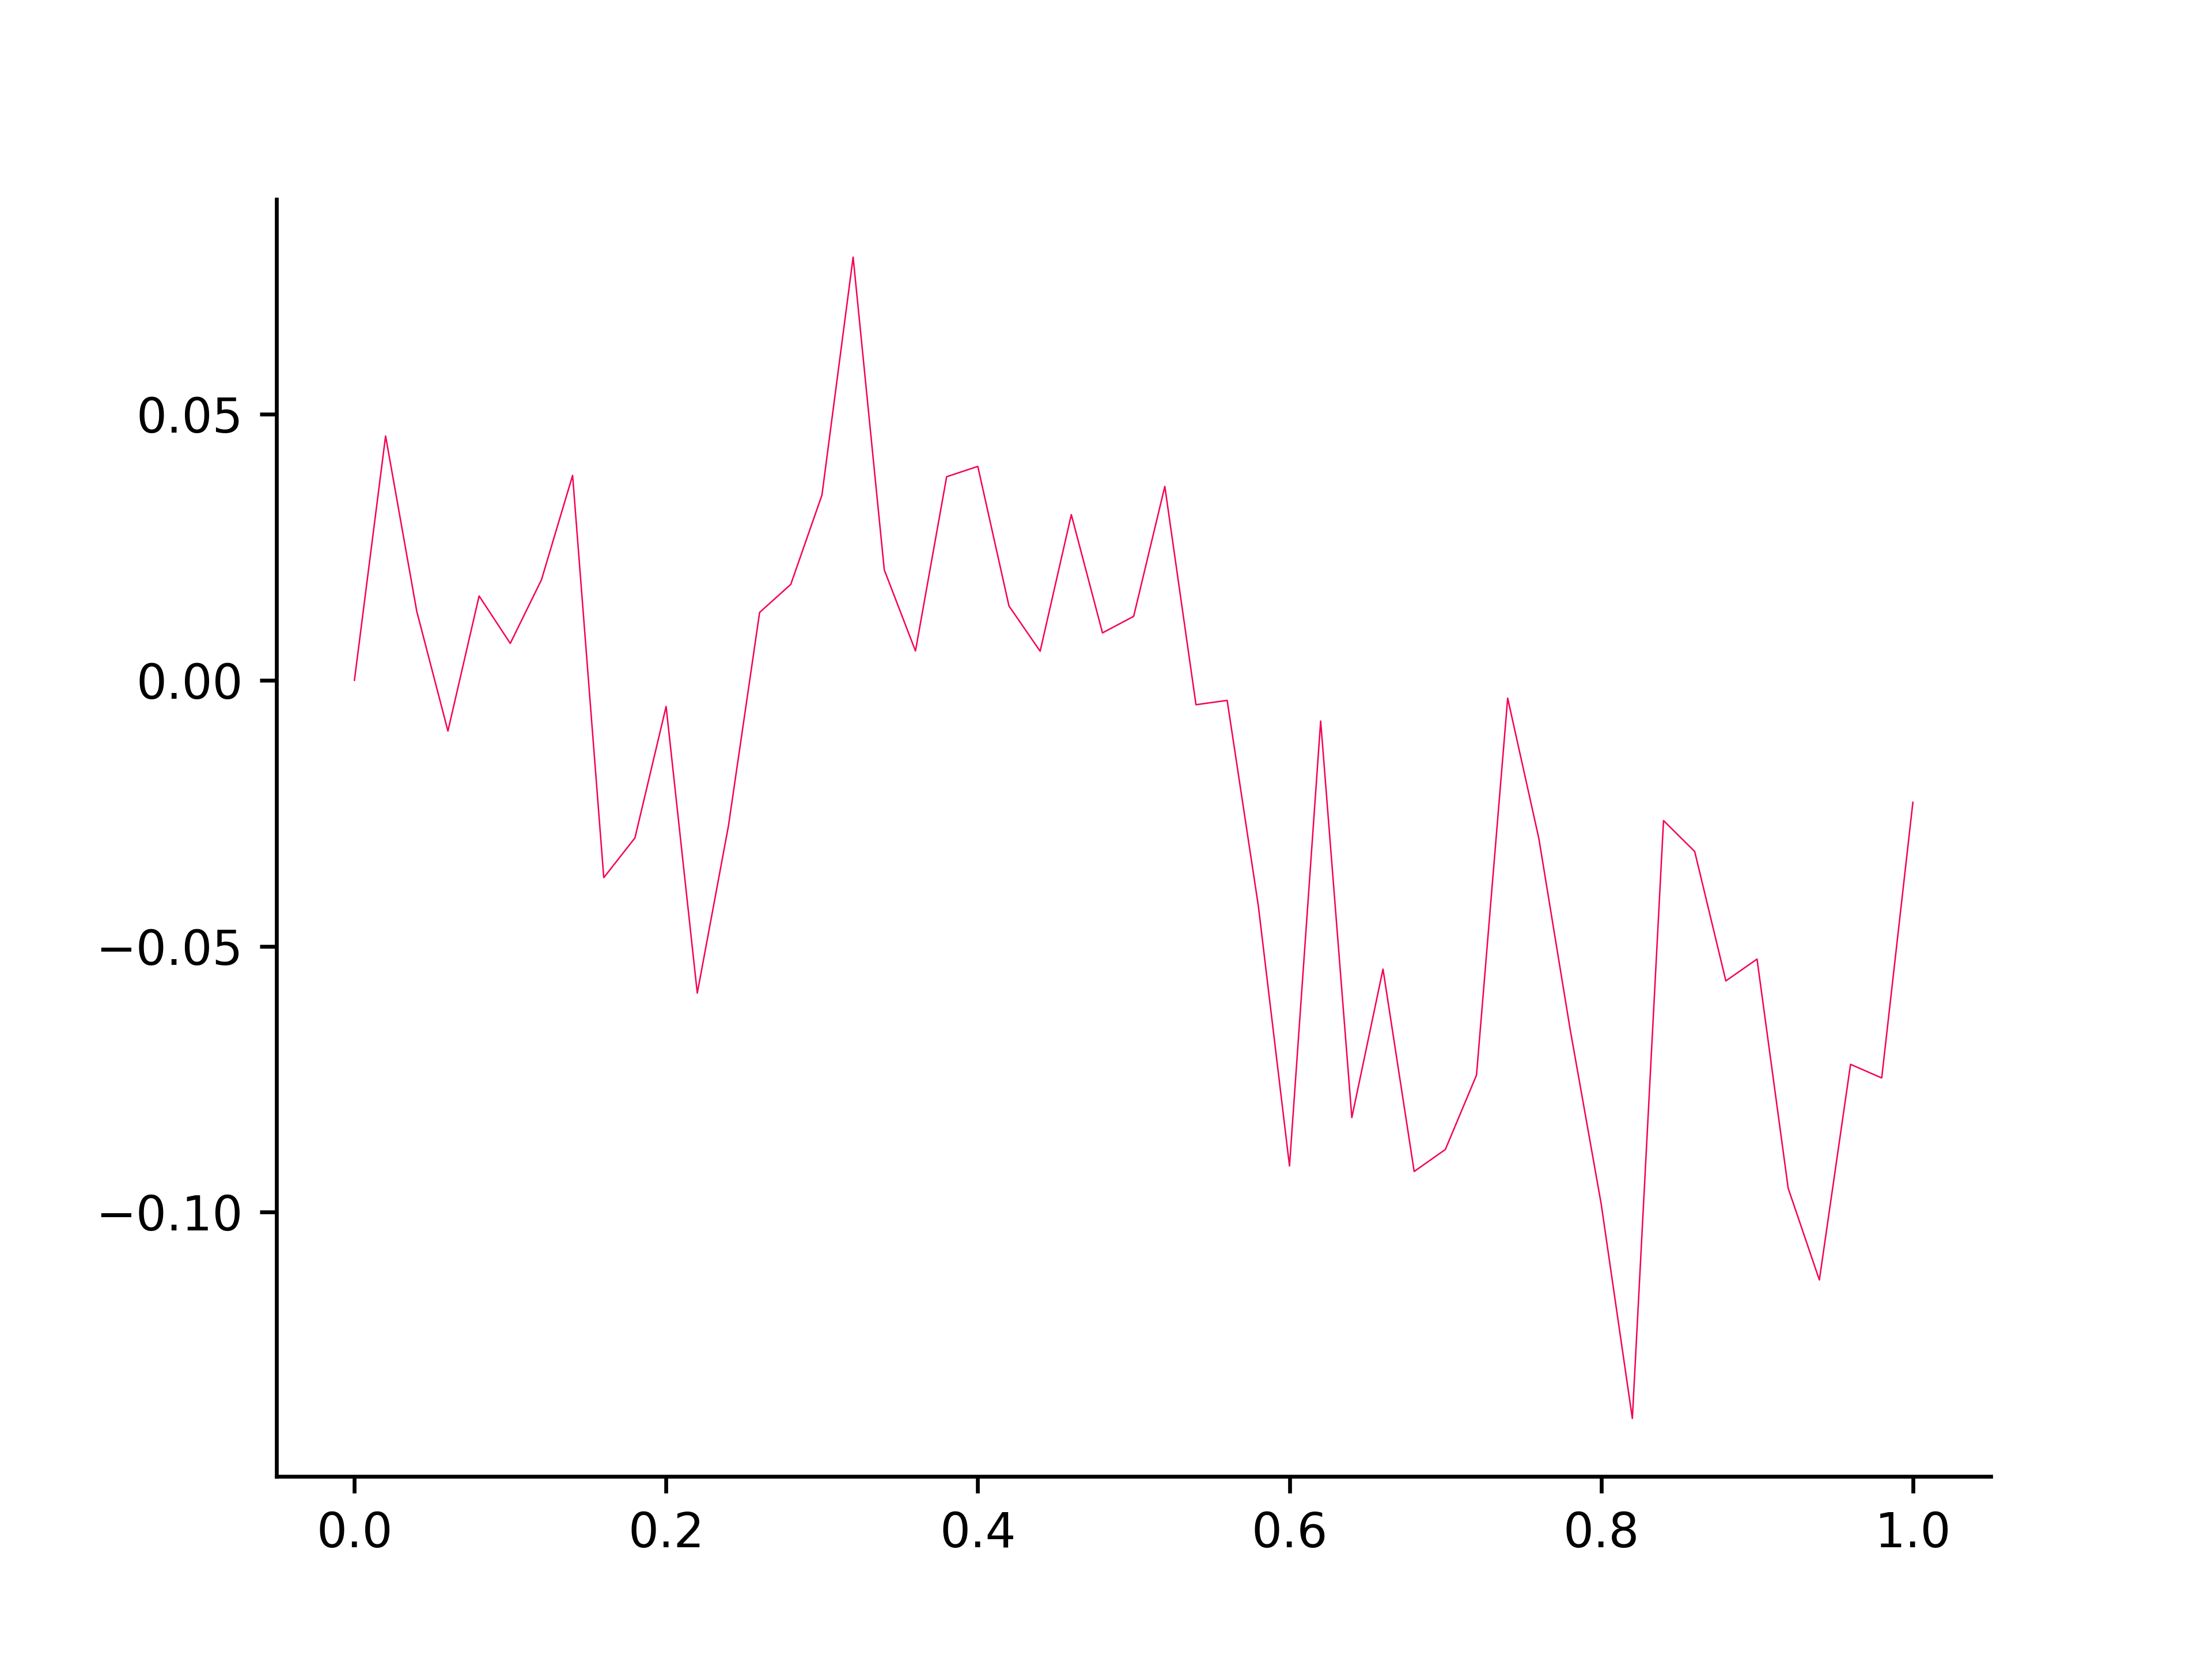
\includegraphics[scale=0.4]{mean-1-25.png}
		\caption{H=0.25}
		\endminipage\hfill
		\minipage{0.49\textwidth}
		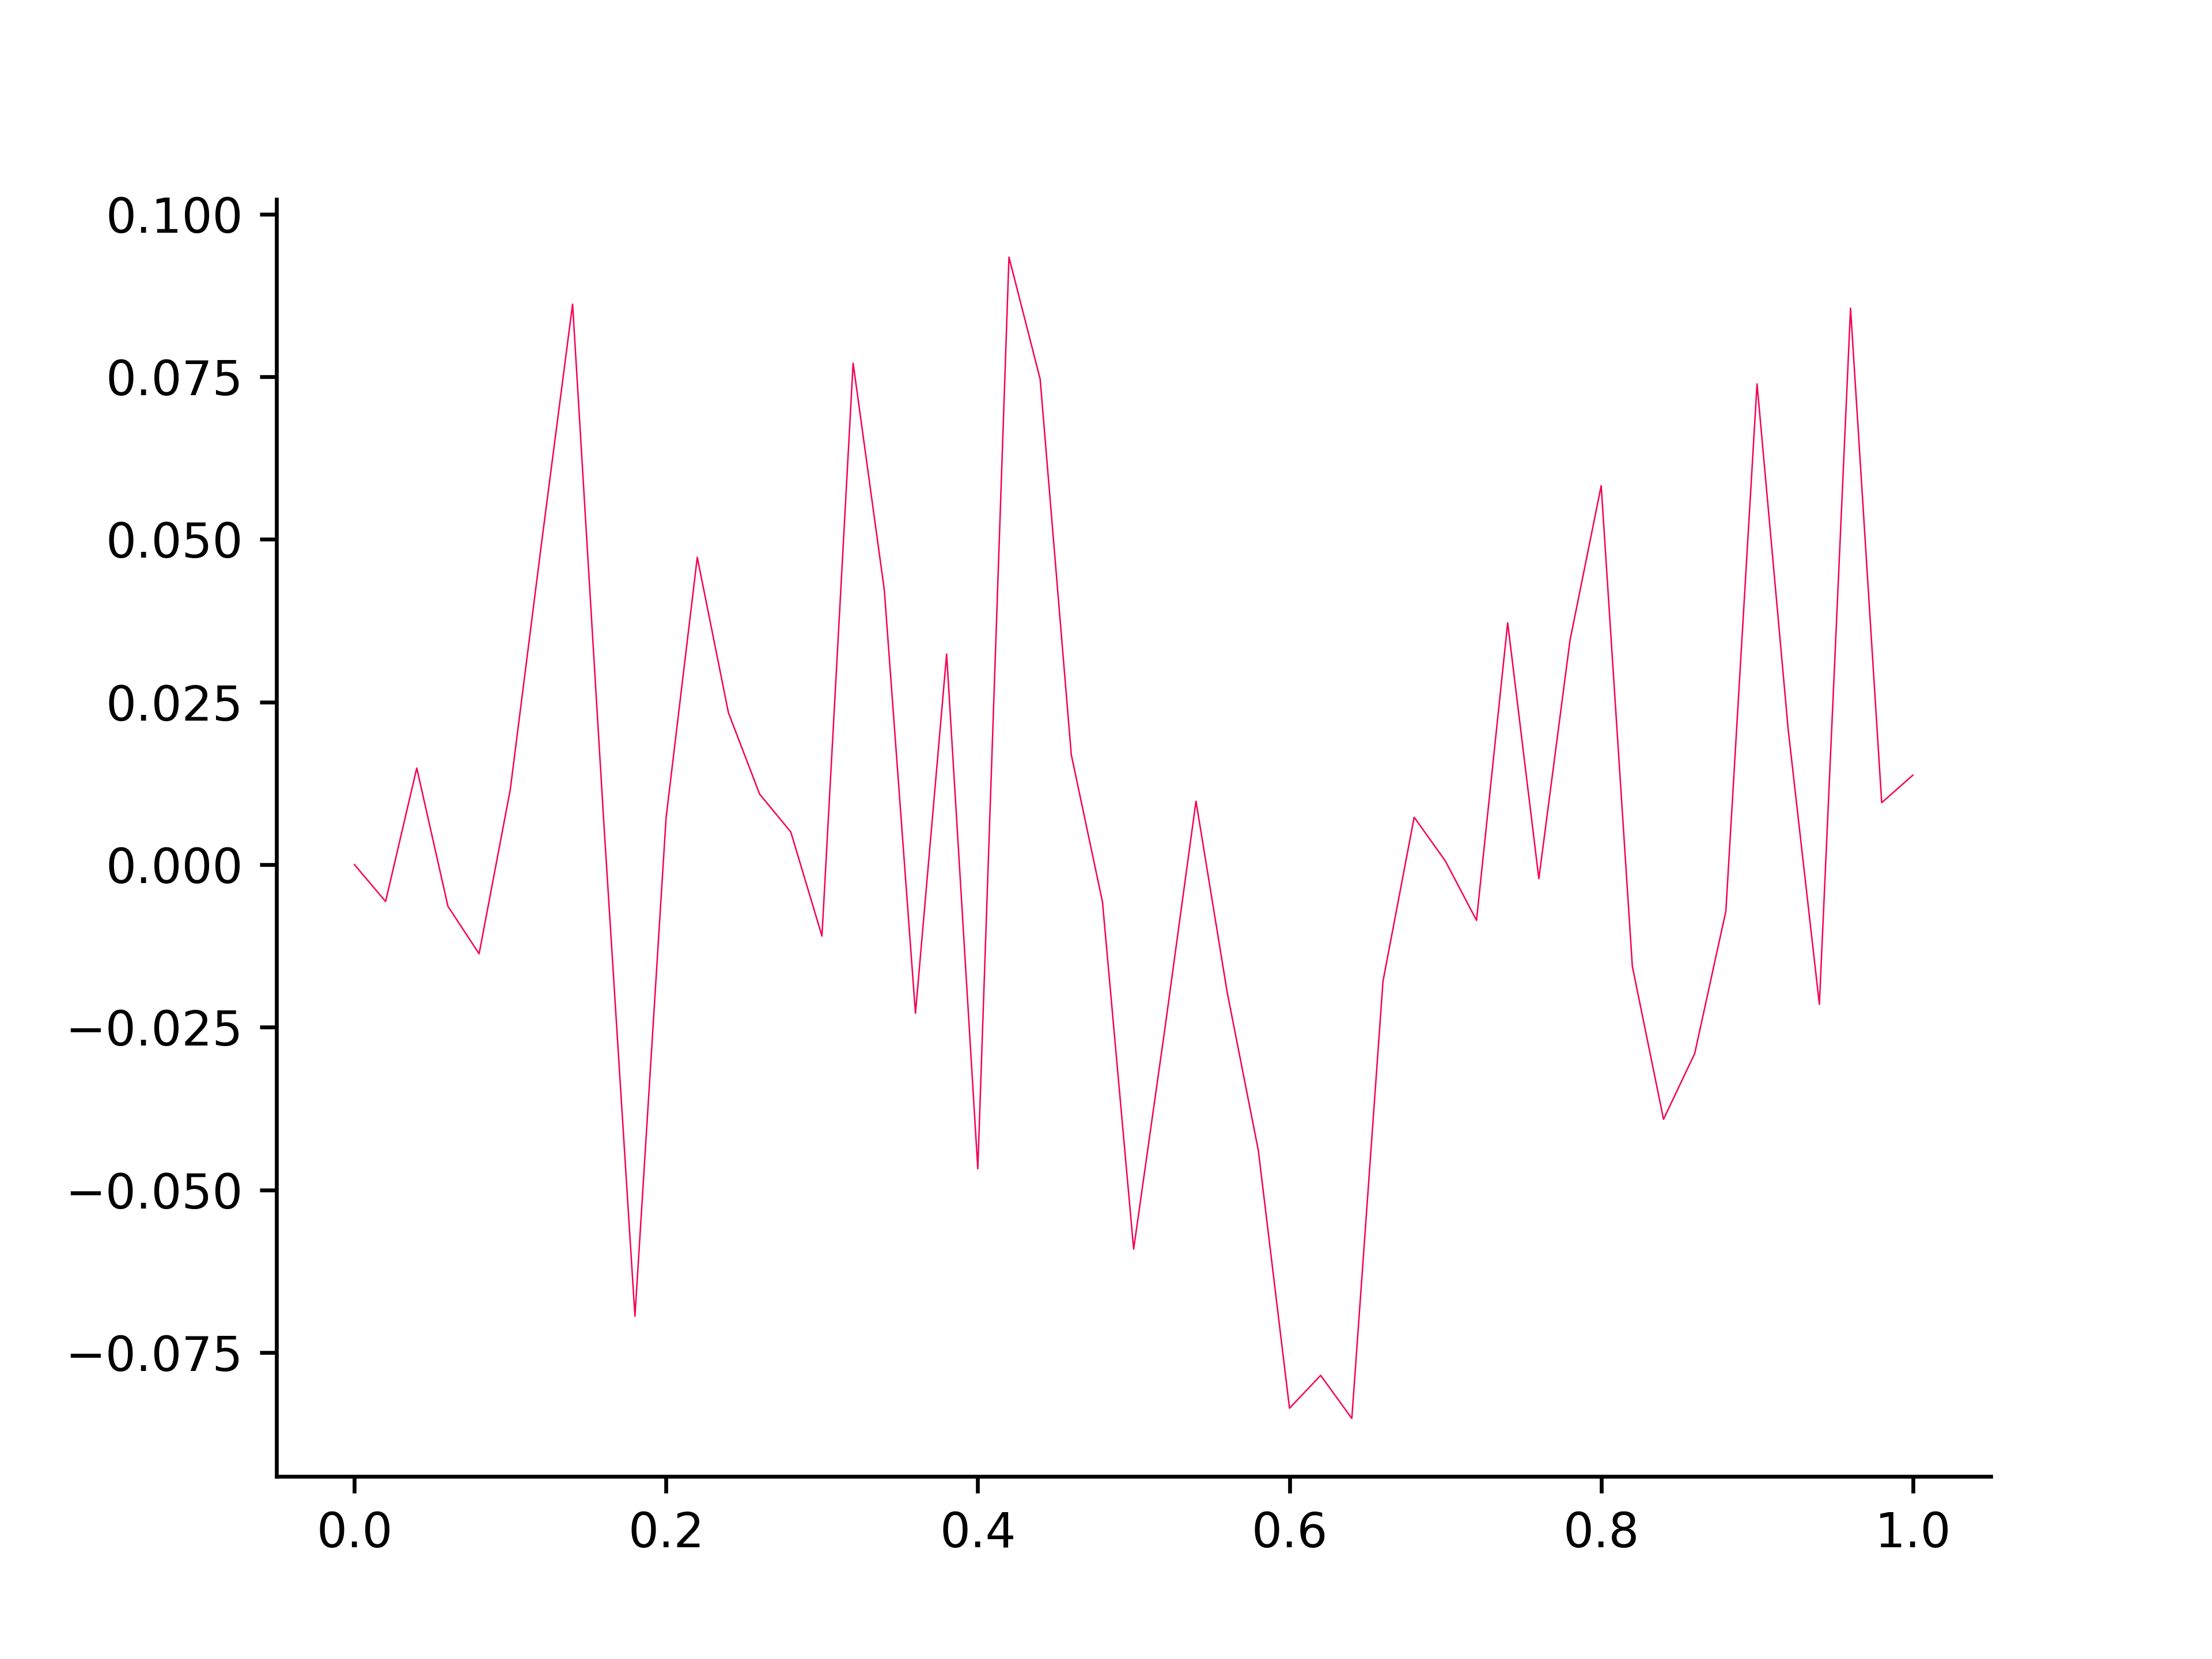
\includegraphics[scale=0.4]{mean-1-05.png}
		\caption{H=0.05}
		\endminipage\hfill
	\end{figure}
	
	\subsection{Второй алгоритм}
	Ниже представлены графики 100 траекторий дробного броуновского движения, смоделированных вторым алгоритмом с параметром $\Theta = 1000$:
	
	Траектории (100 шт.):
	\begin{figure}[H]
		\minipage{0.49\textwidth}
		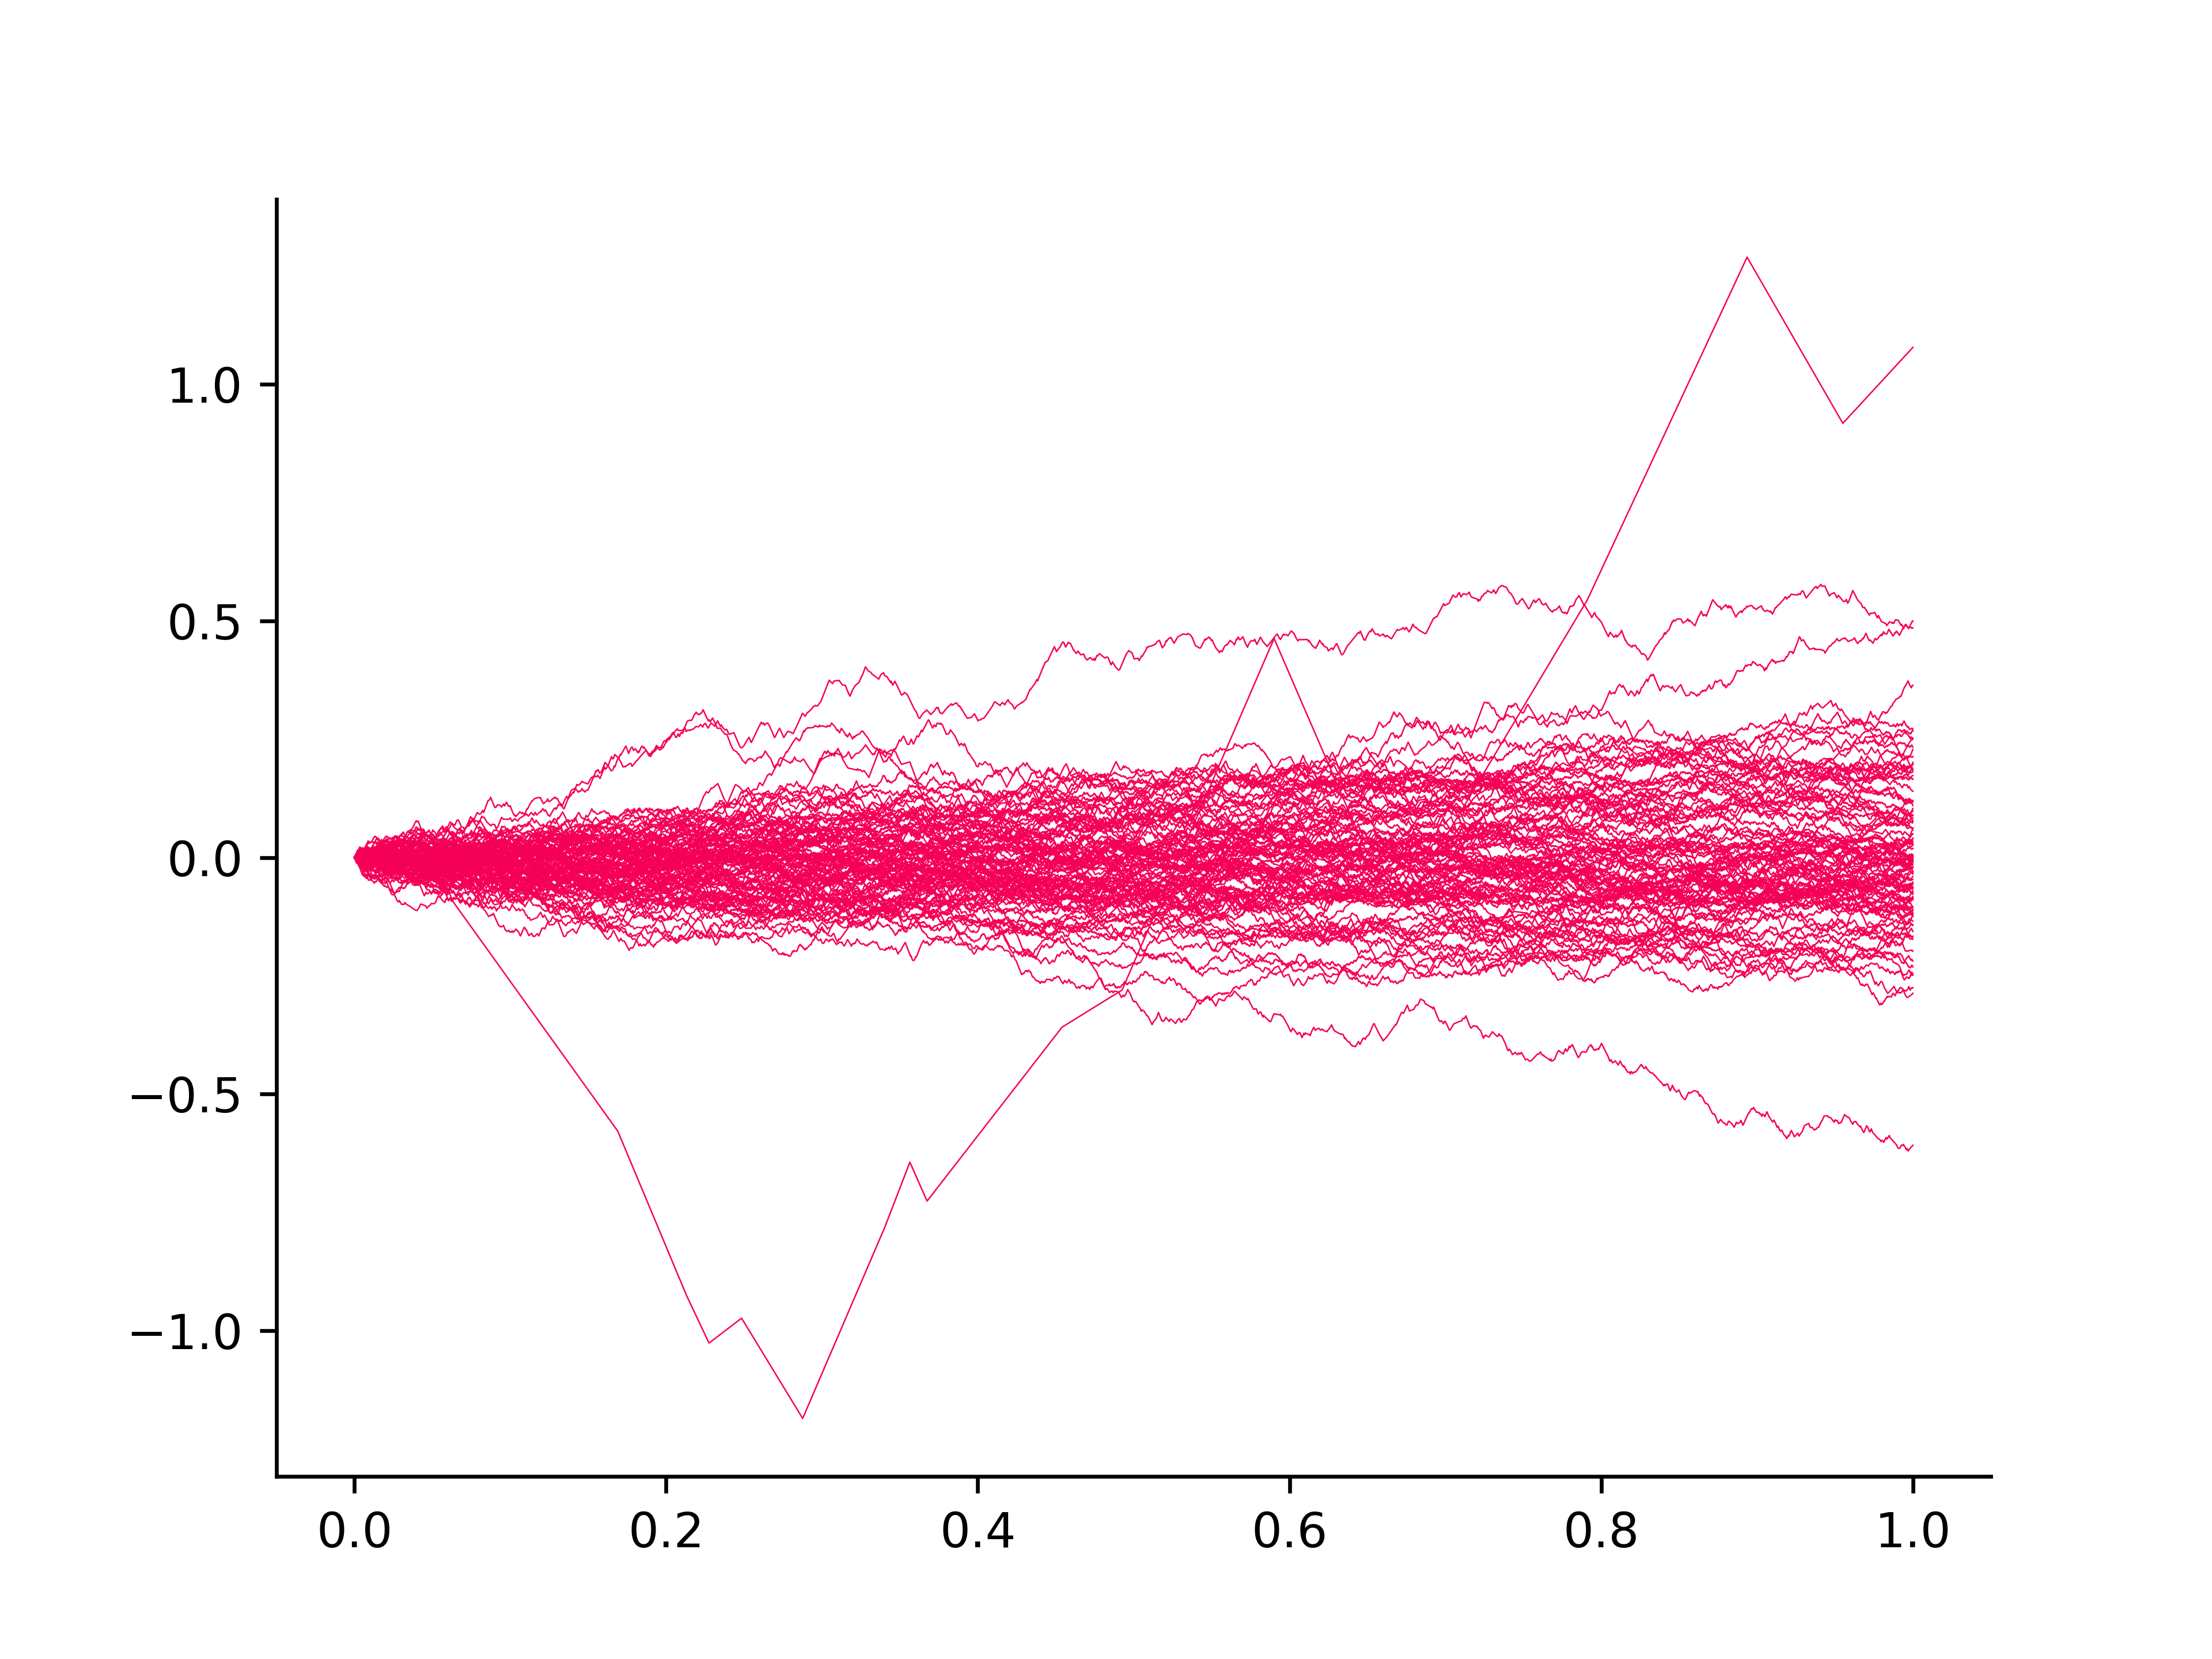
\includegraphics[scale=0.4]{image-2-55.png}
		\caption{H=0.55}
		\endminipage\hfill
		\minipage{0.49\textwidth}
		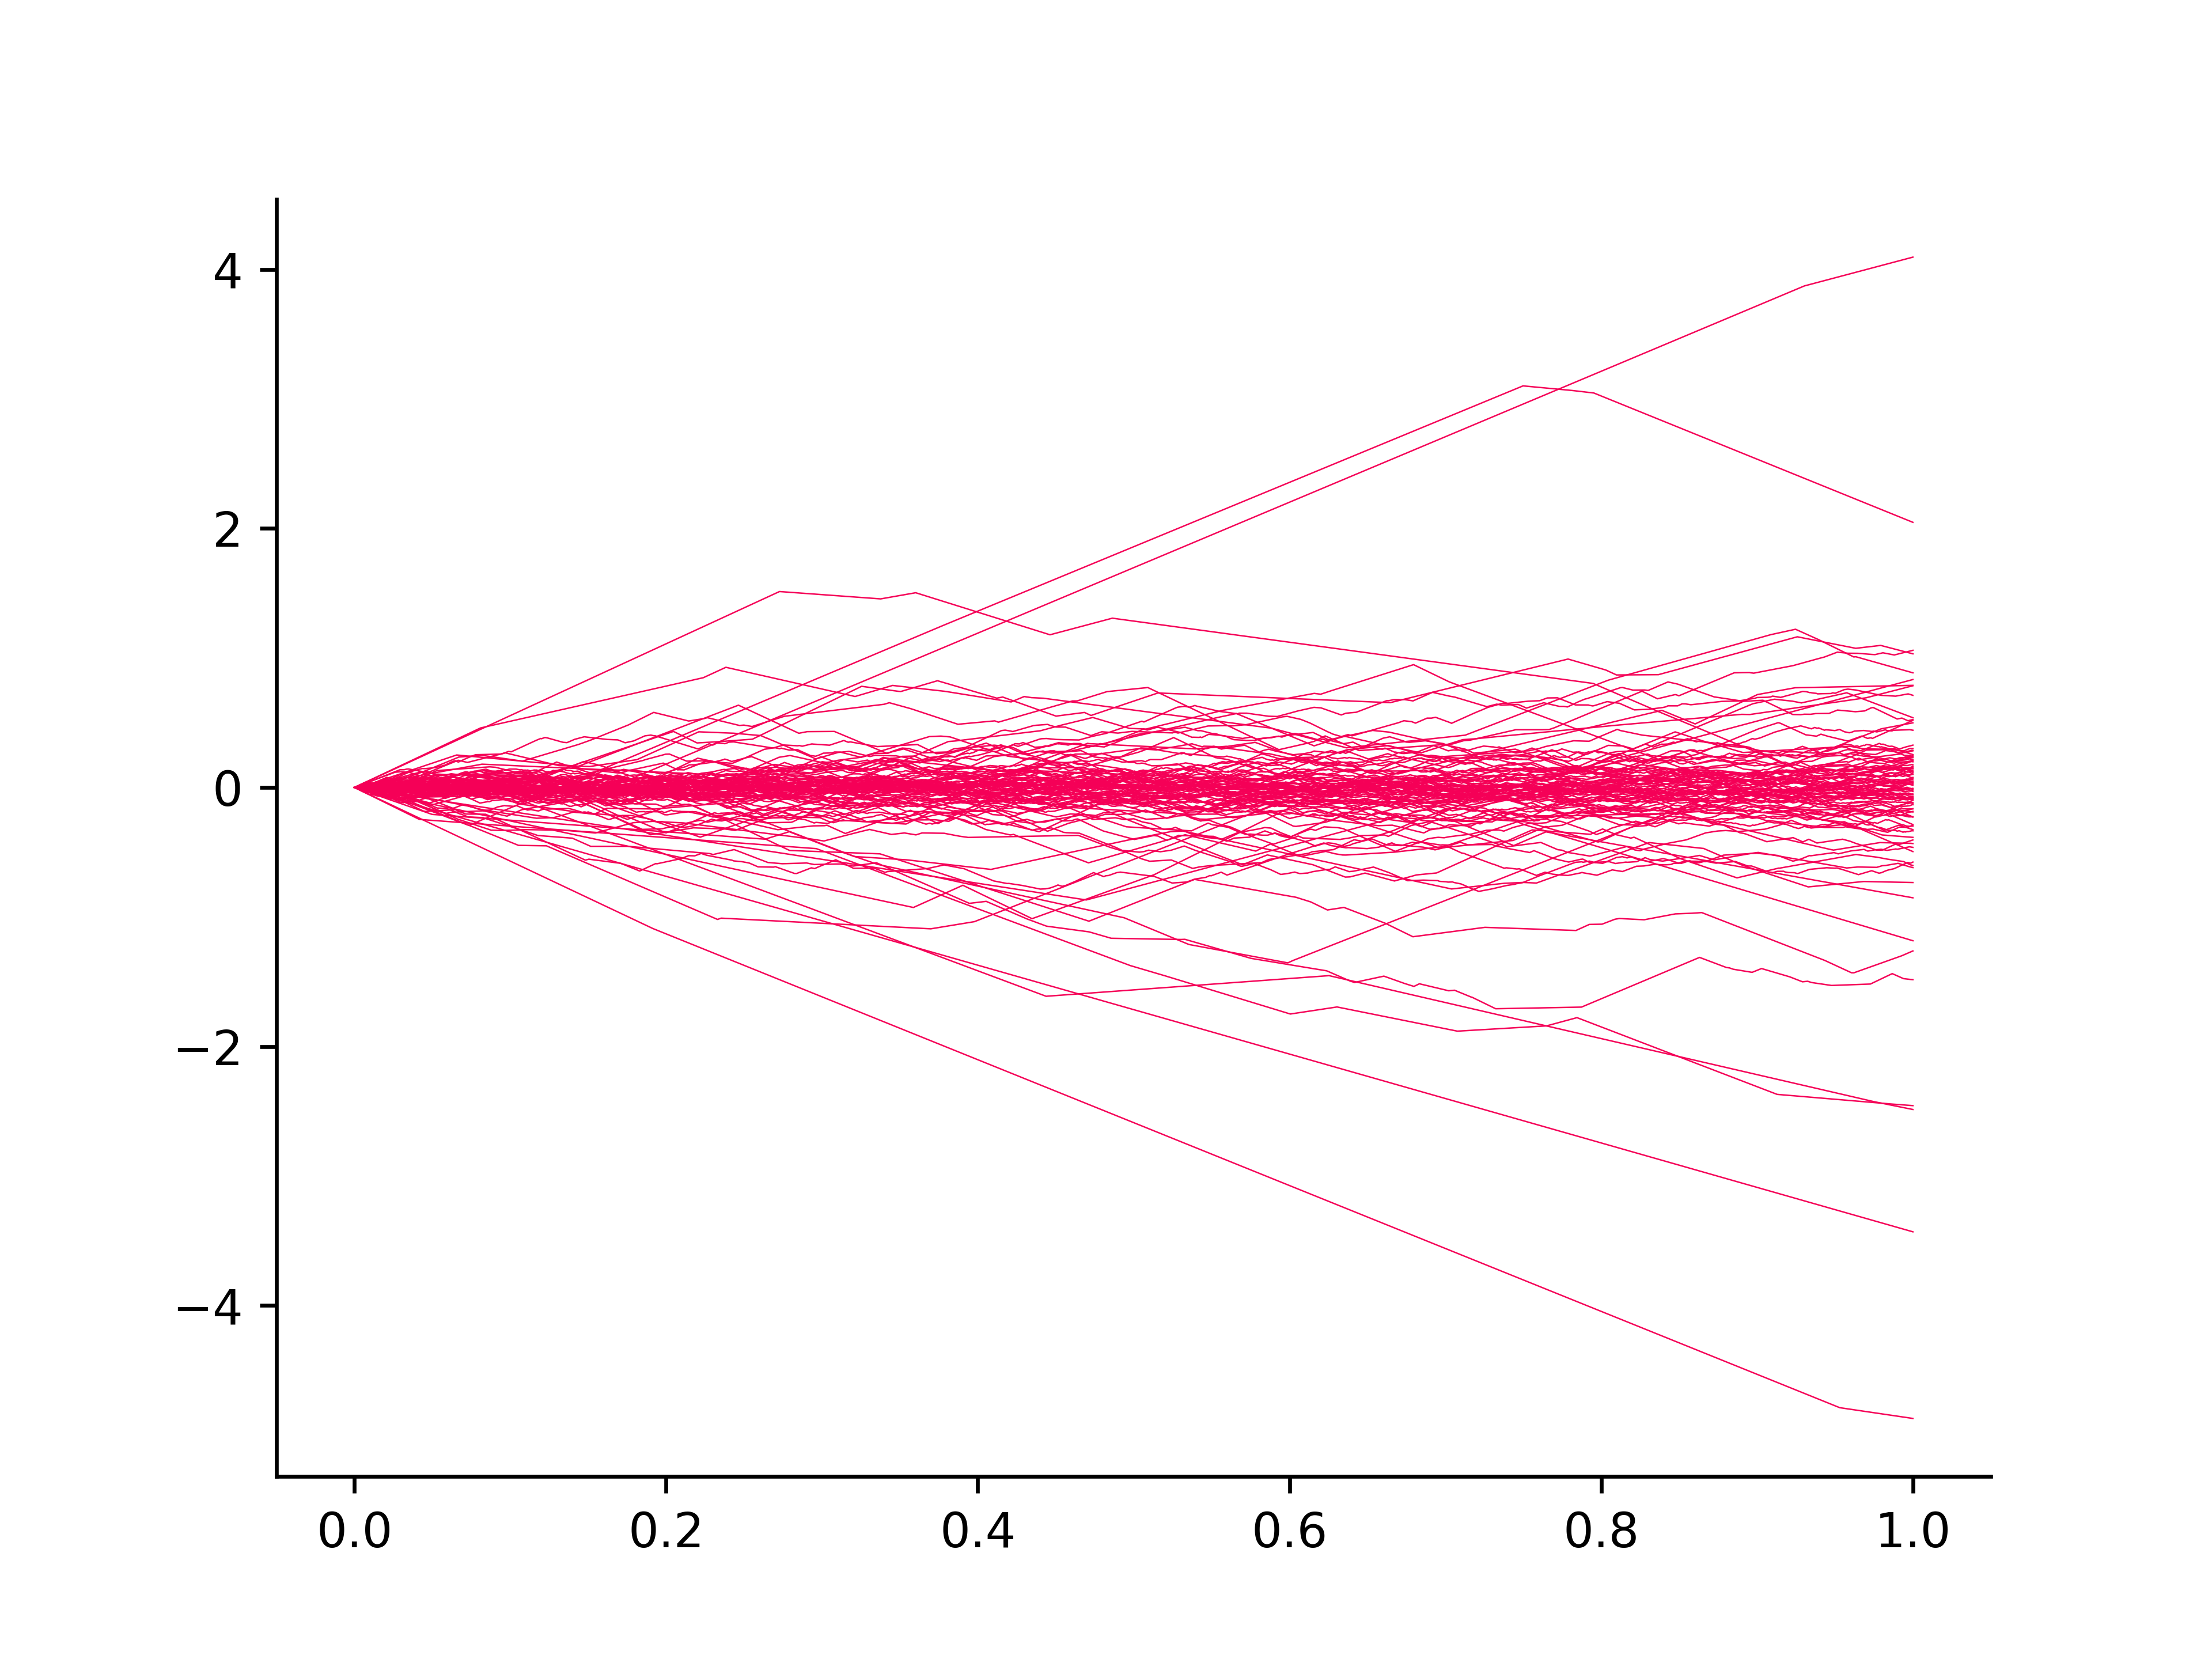
\includegraphics[scale=0.4]{image-2-75.png}
		\caption{H=0.75}
		\endminipage\hfill
	\end{figure}
	
	\begin{figure}[H]
		\center
		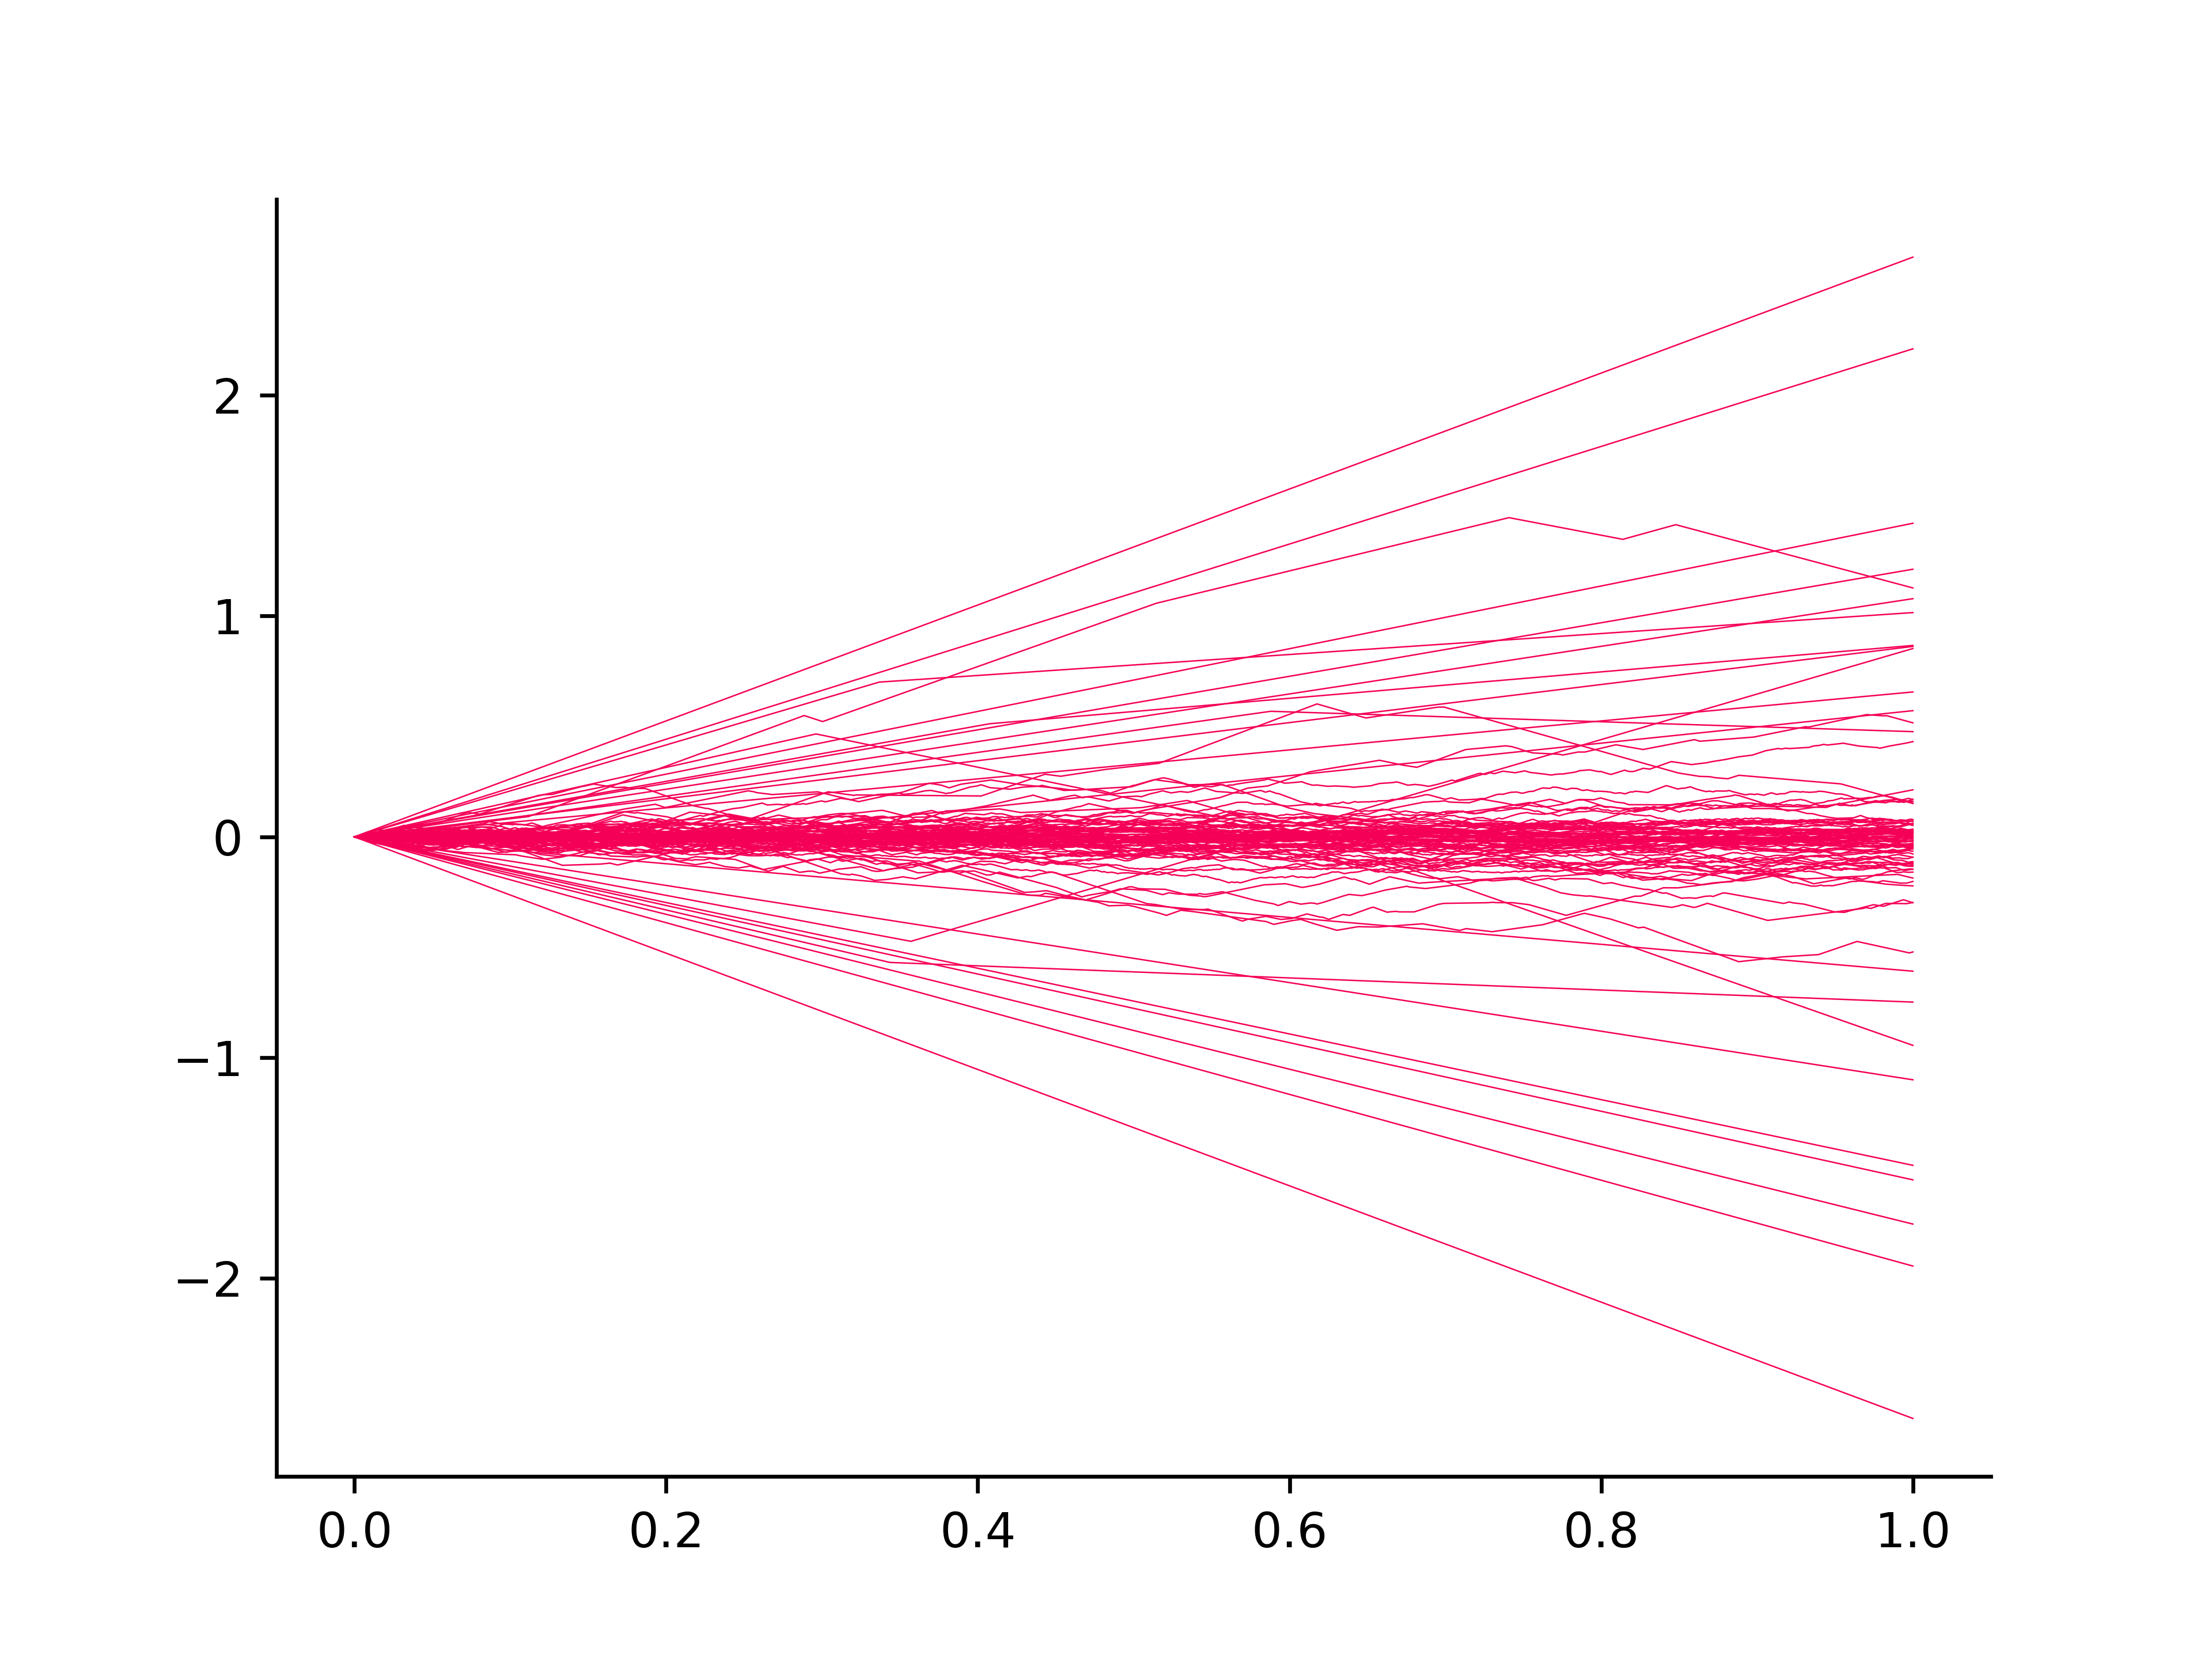
\includegraphics[scale=0.4]{image-2-85.png}
		\caption{H=0.85}
	\end{figure}
	
	Выборочный коэффициент ковариации:
	\begin{figure}[H]
		\minipage{0.49\textwidth}
		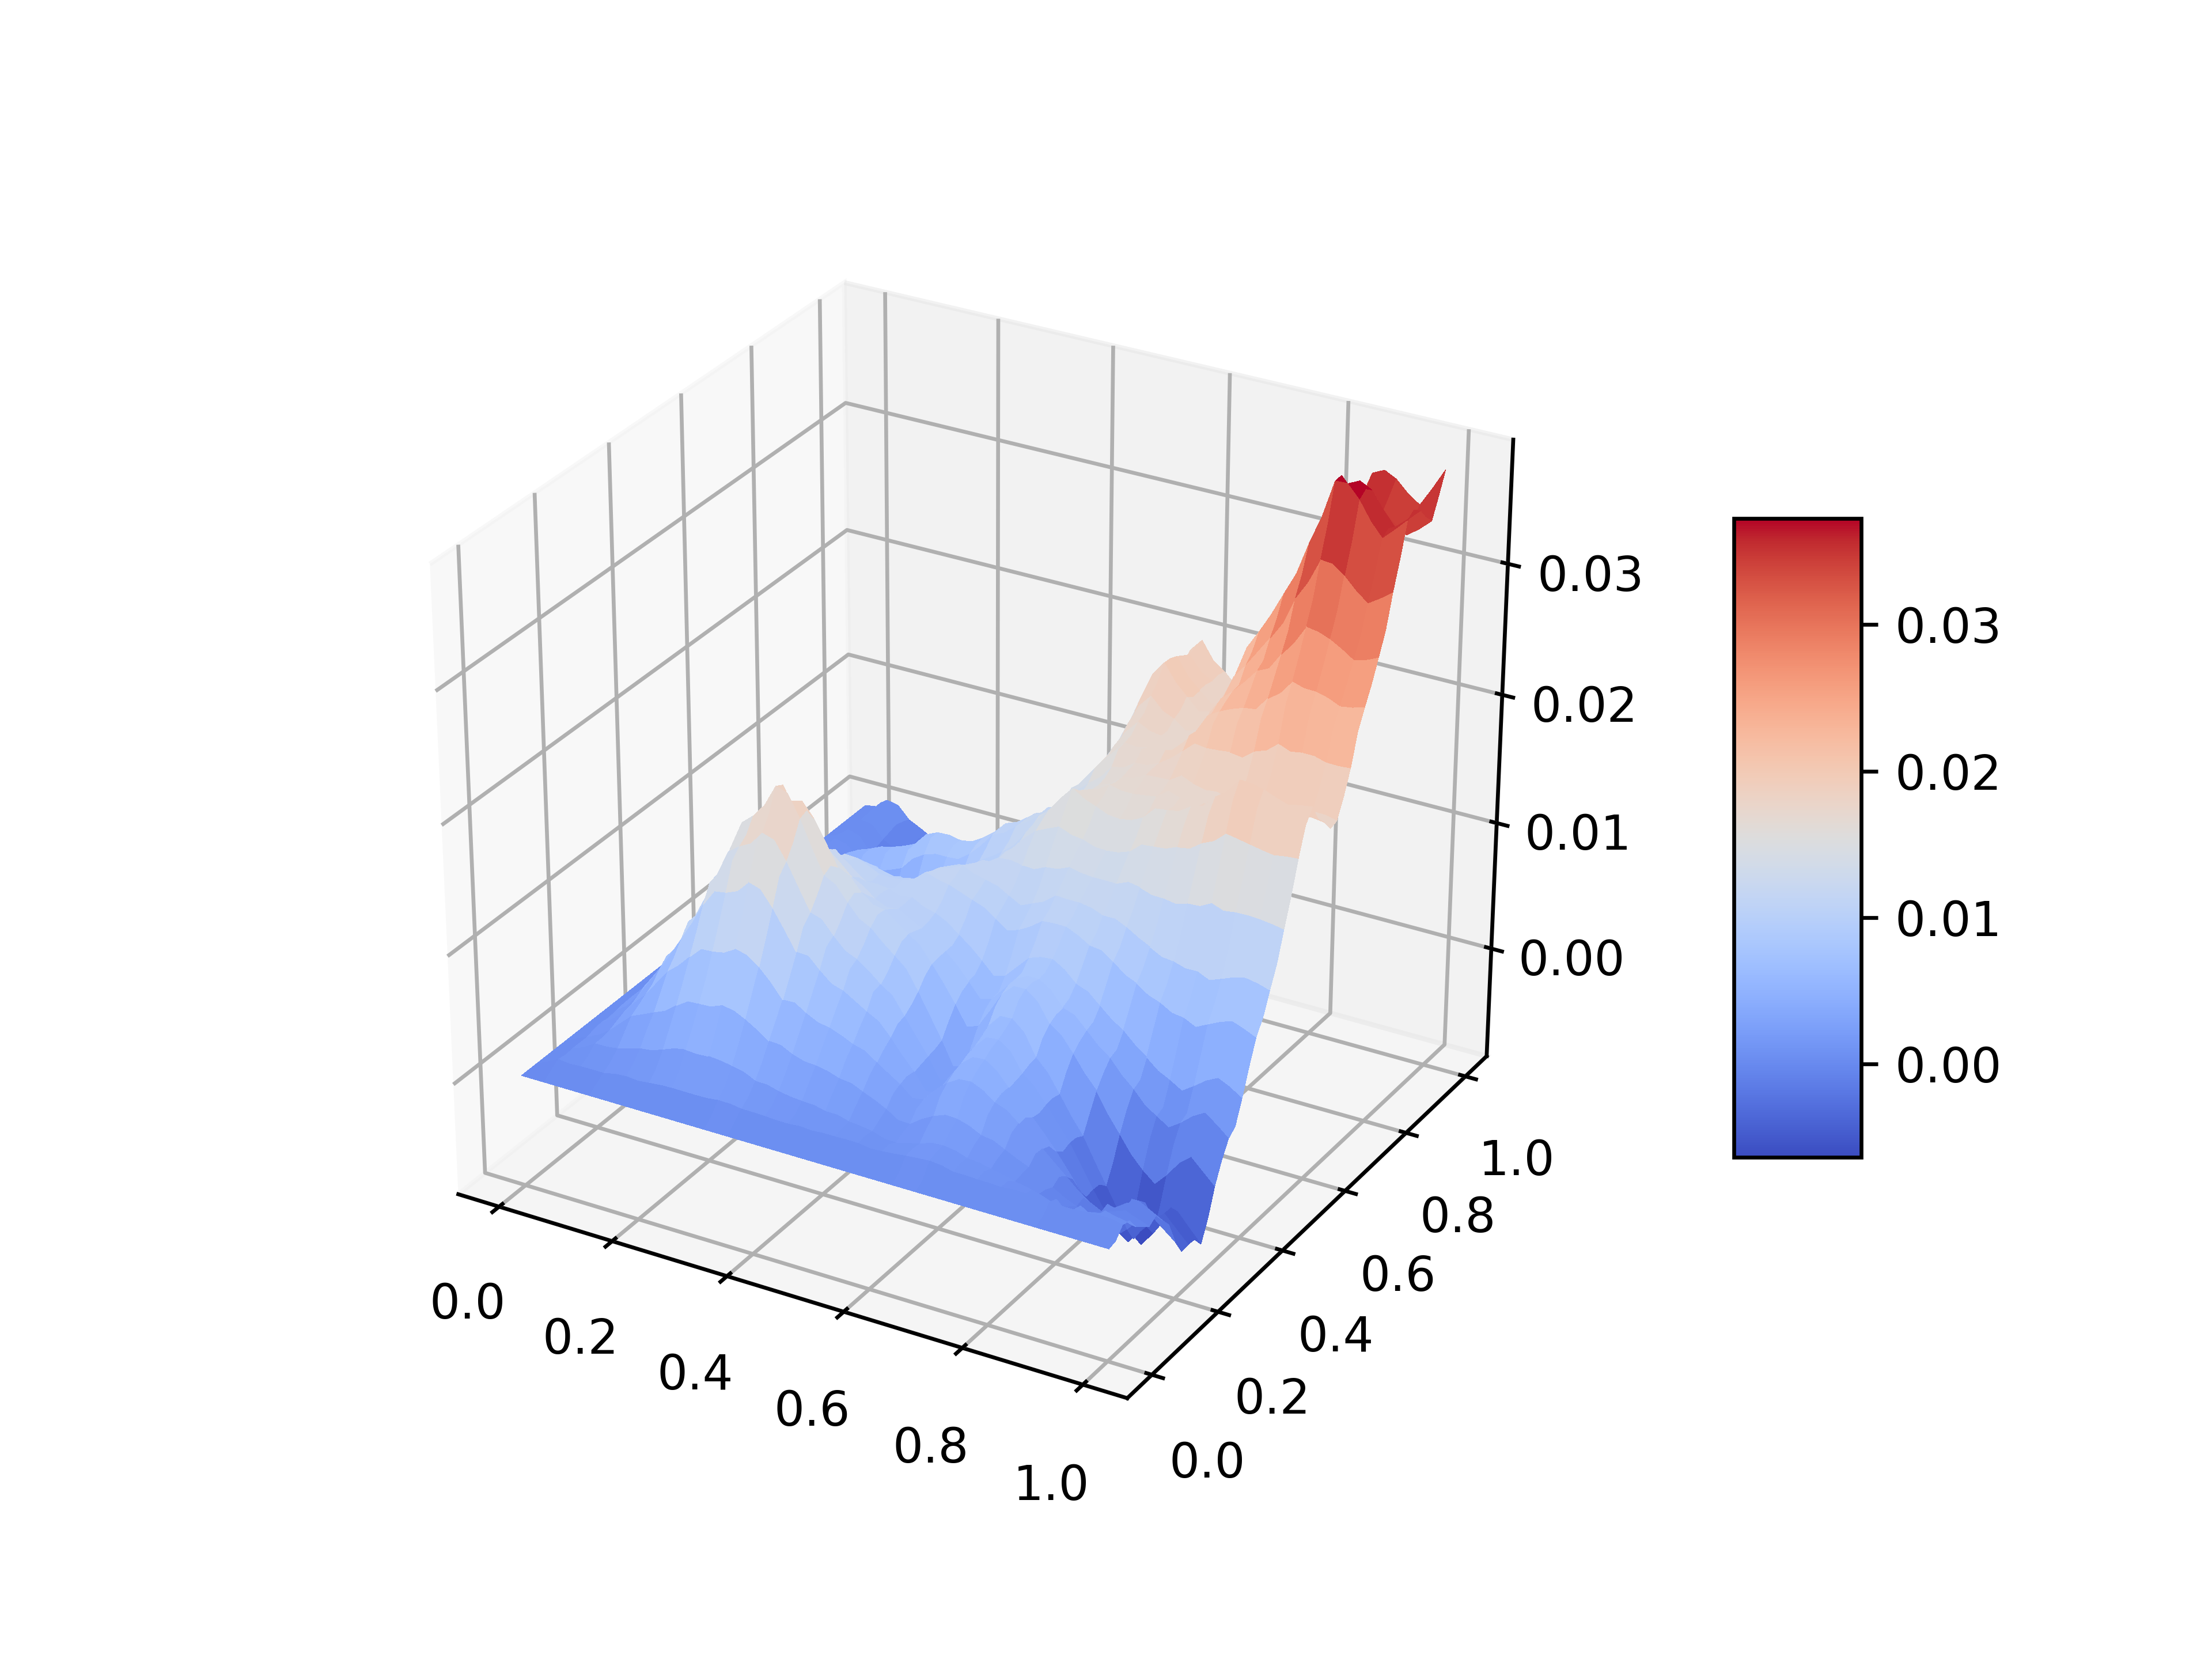
\includegraphics[scale=0.4]{covariance-2-55.png}
		\caption{H=0.55}
		\endminipage\hfill
		\minipage{0.49\textwidth}
		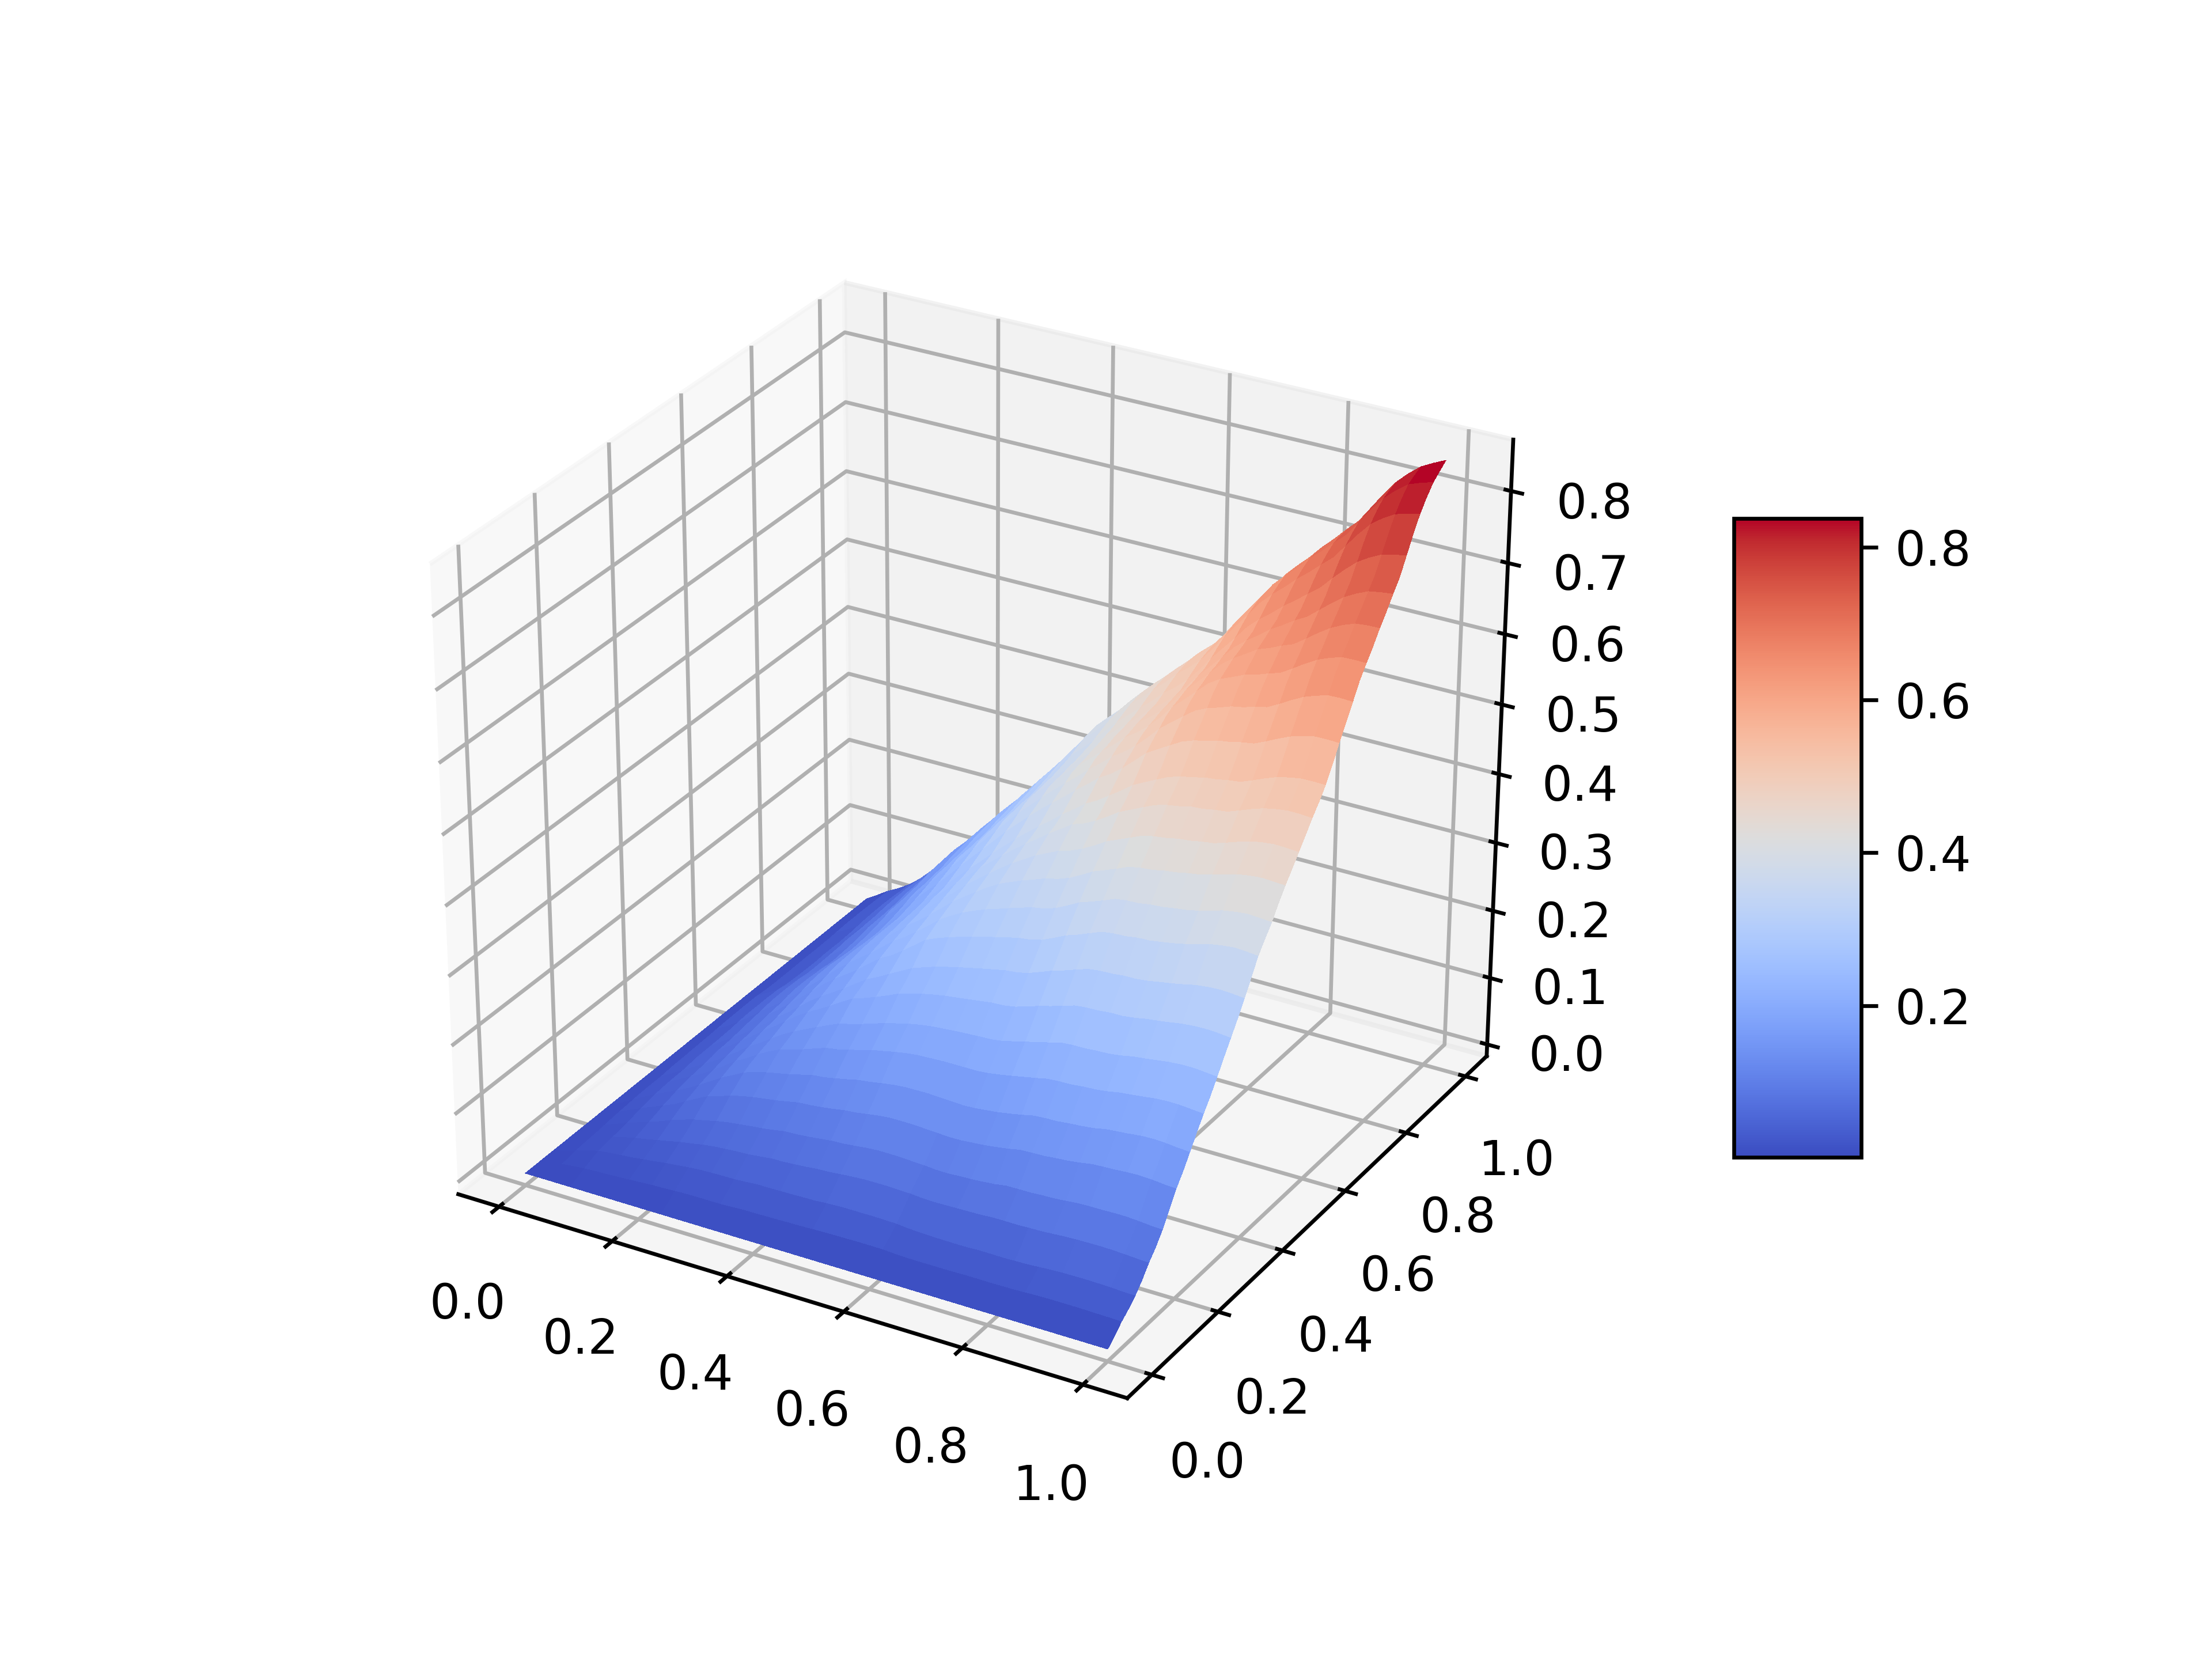
\includegraphics[scale=0.4]{covariance-2-75.png}
		\caption{H=0.75}
		\endminipage\hfill
	\end{figure}
	
	\begin{figure}[H]
		\center
		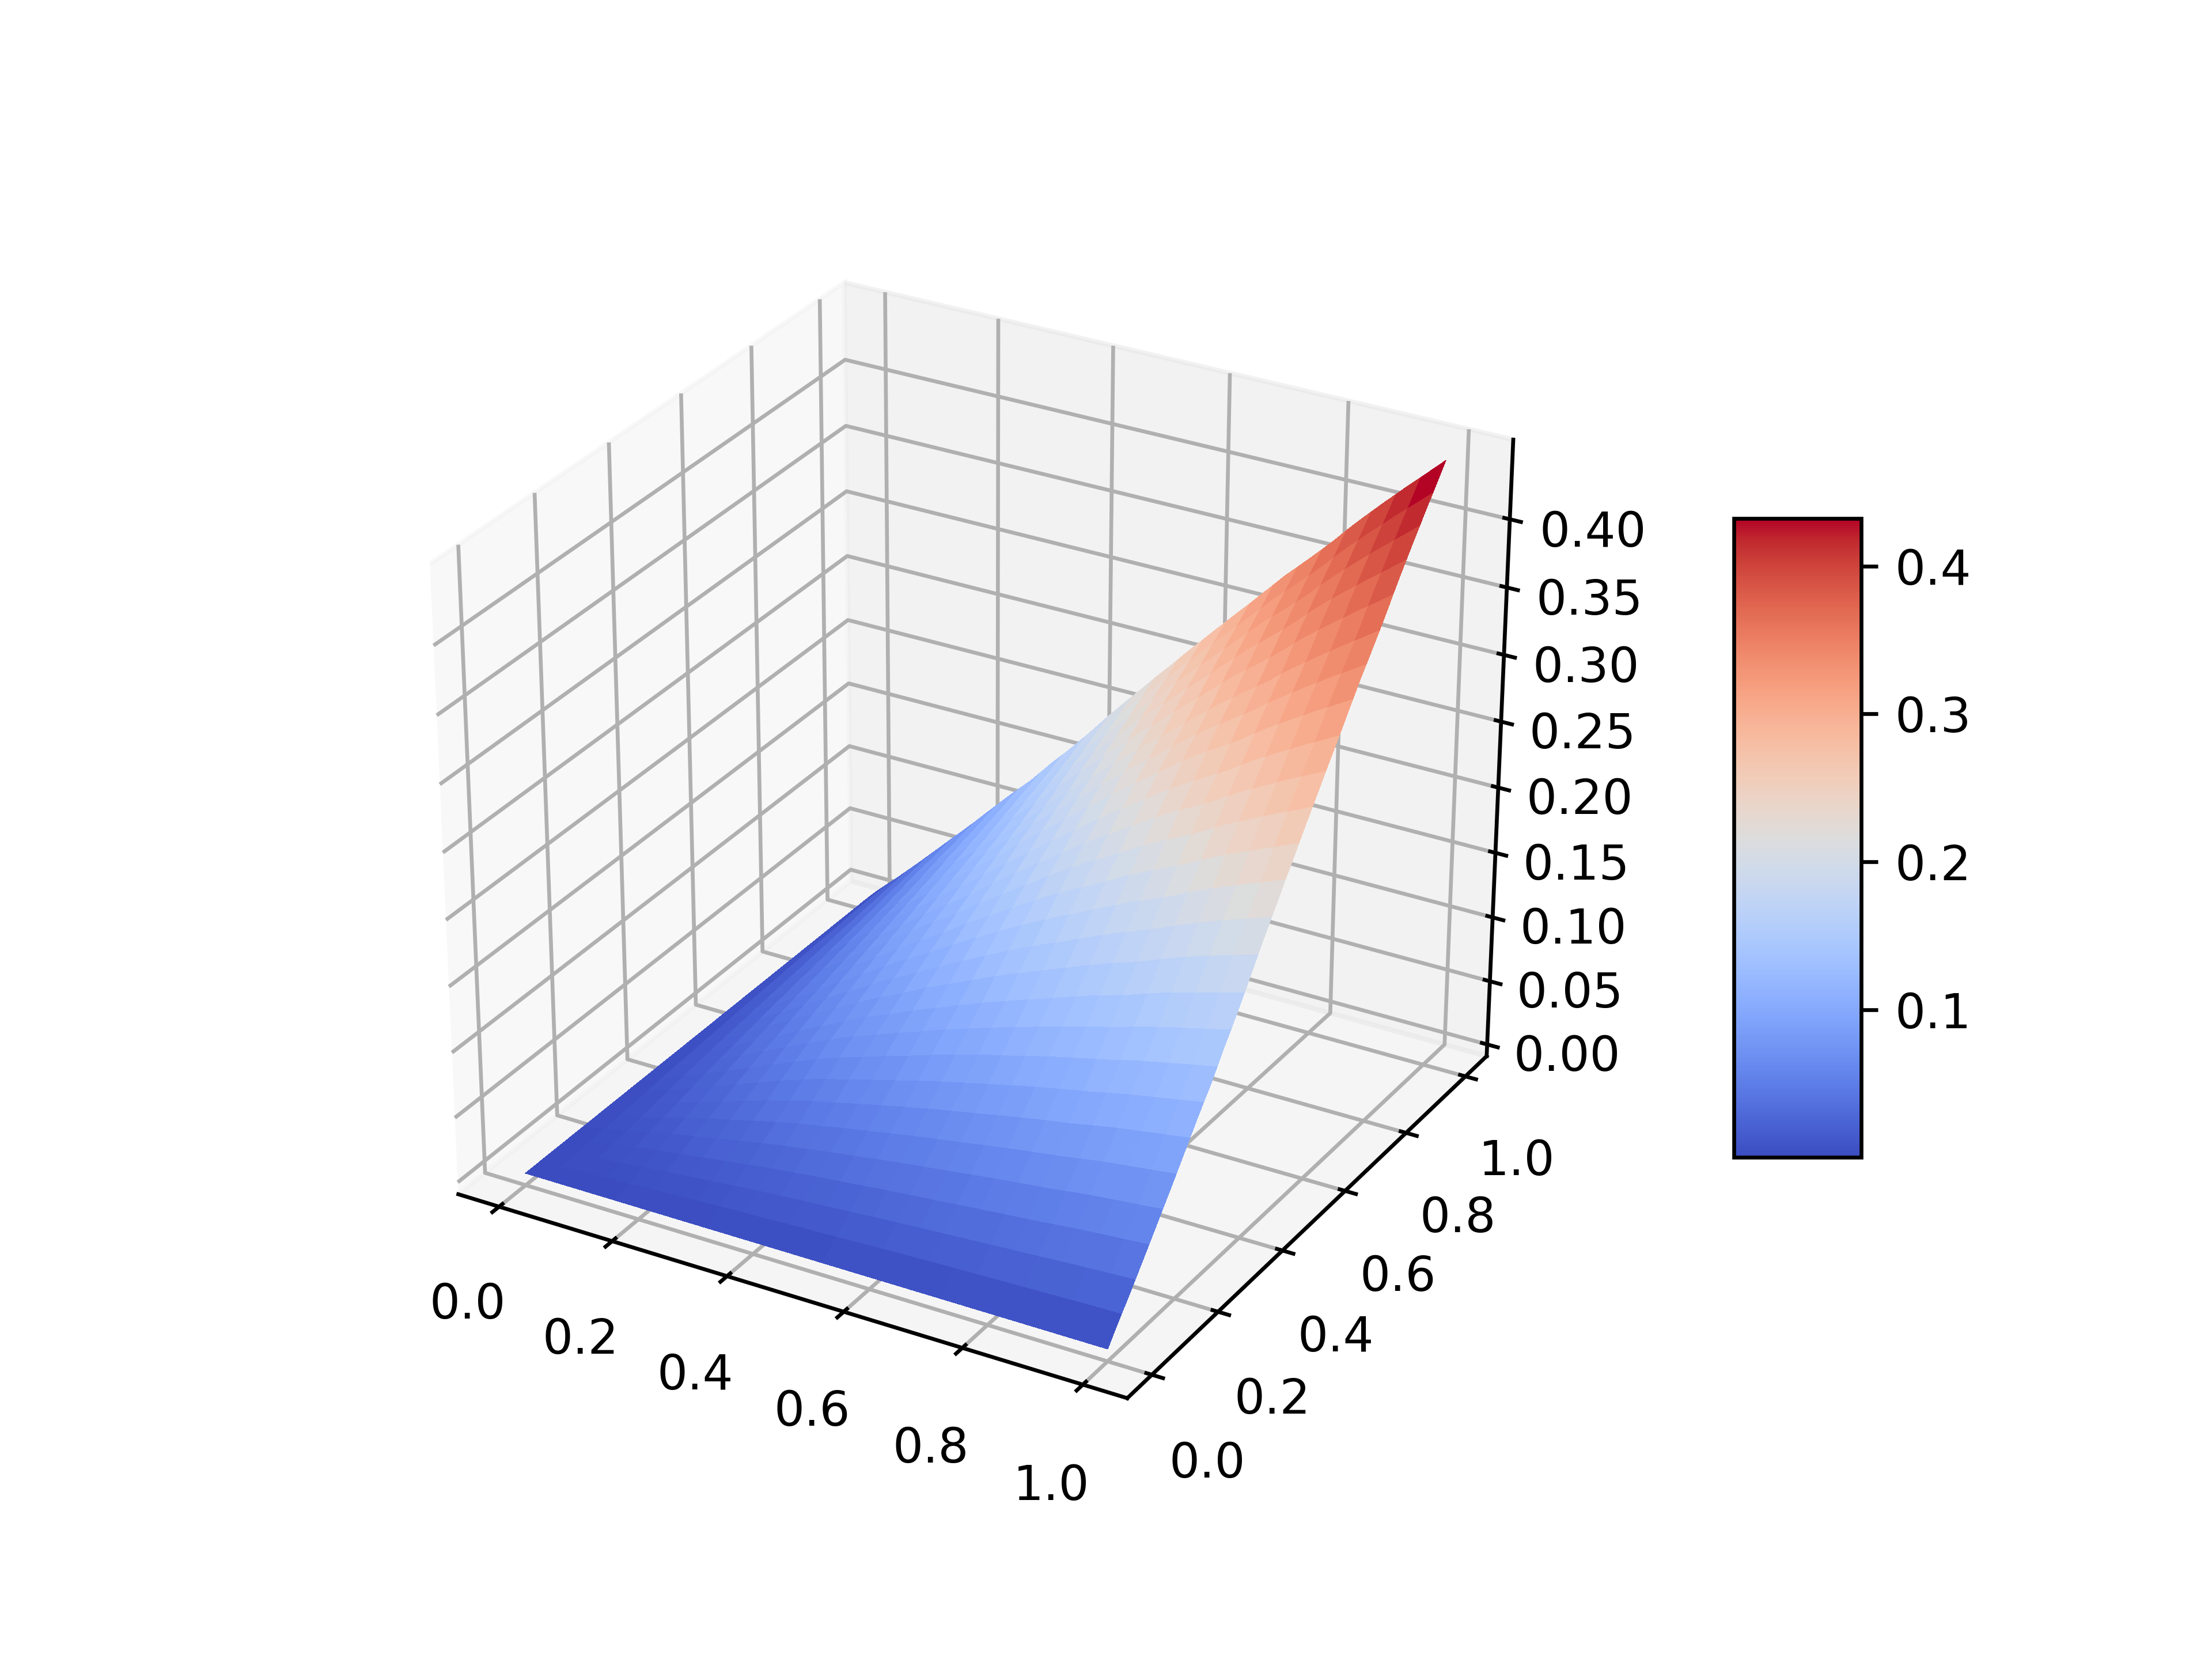
\includegraphics[scale=0.4]{covariance-2-85.png}
		\caption{H=0.85}
	\end{figure}
	
	Выборочное среднее:
	\begin{figure}[H]
		\minipage{0.49\textwidth}
		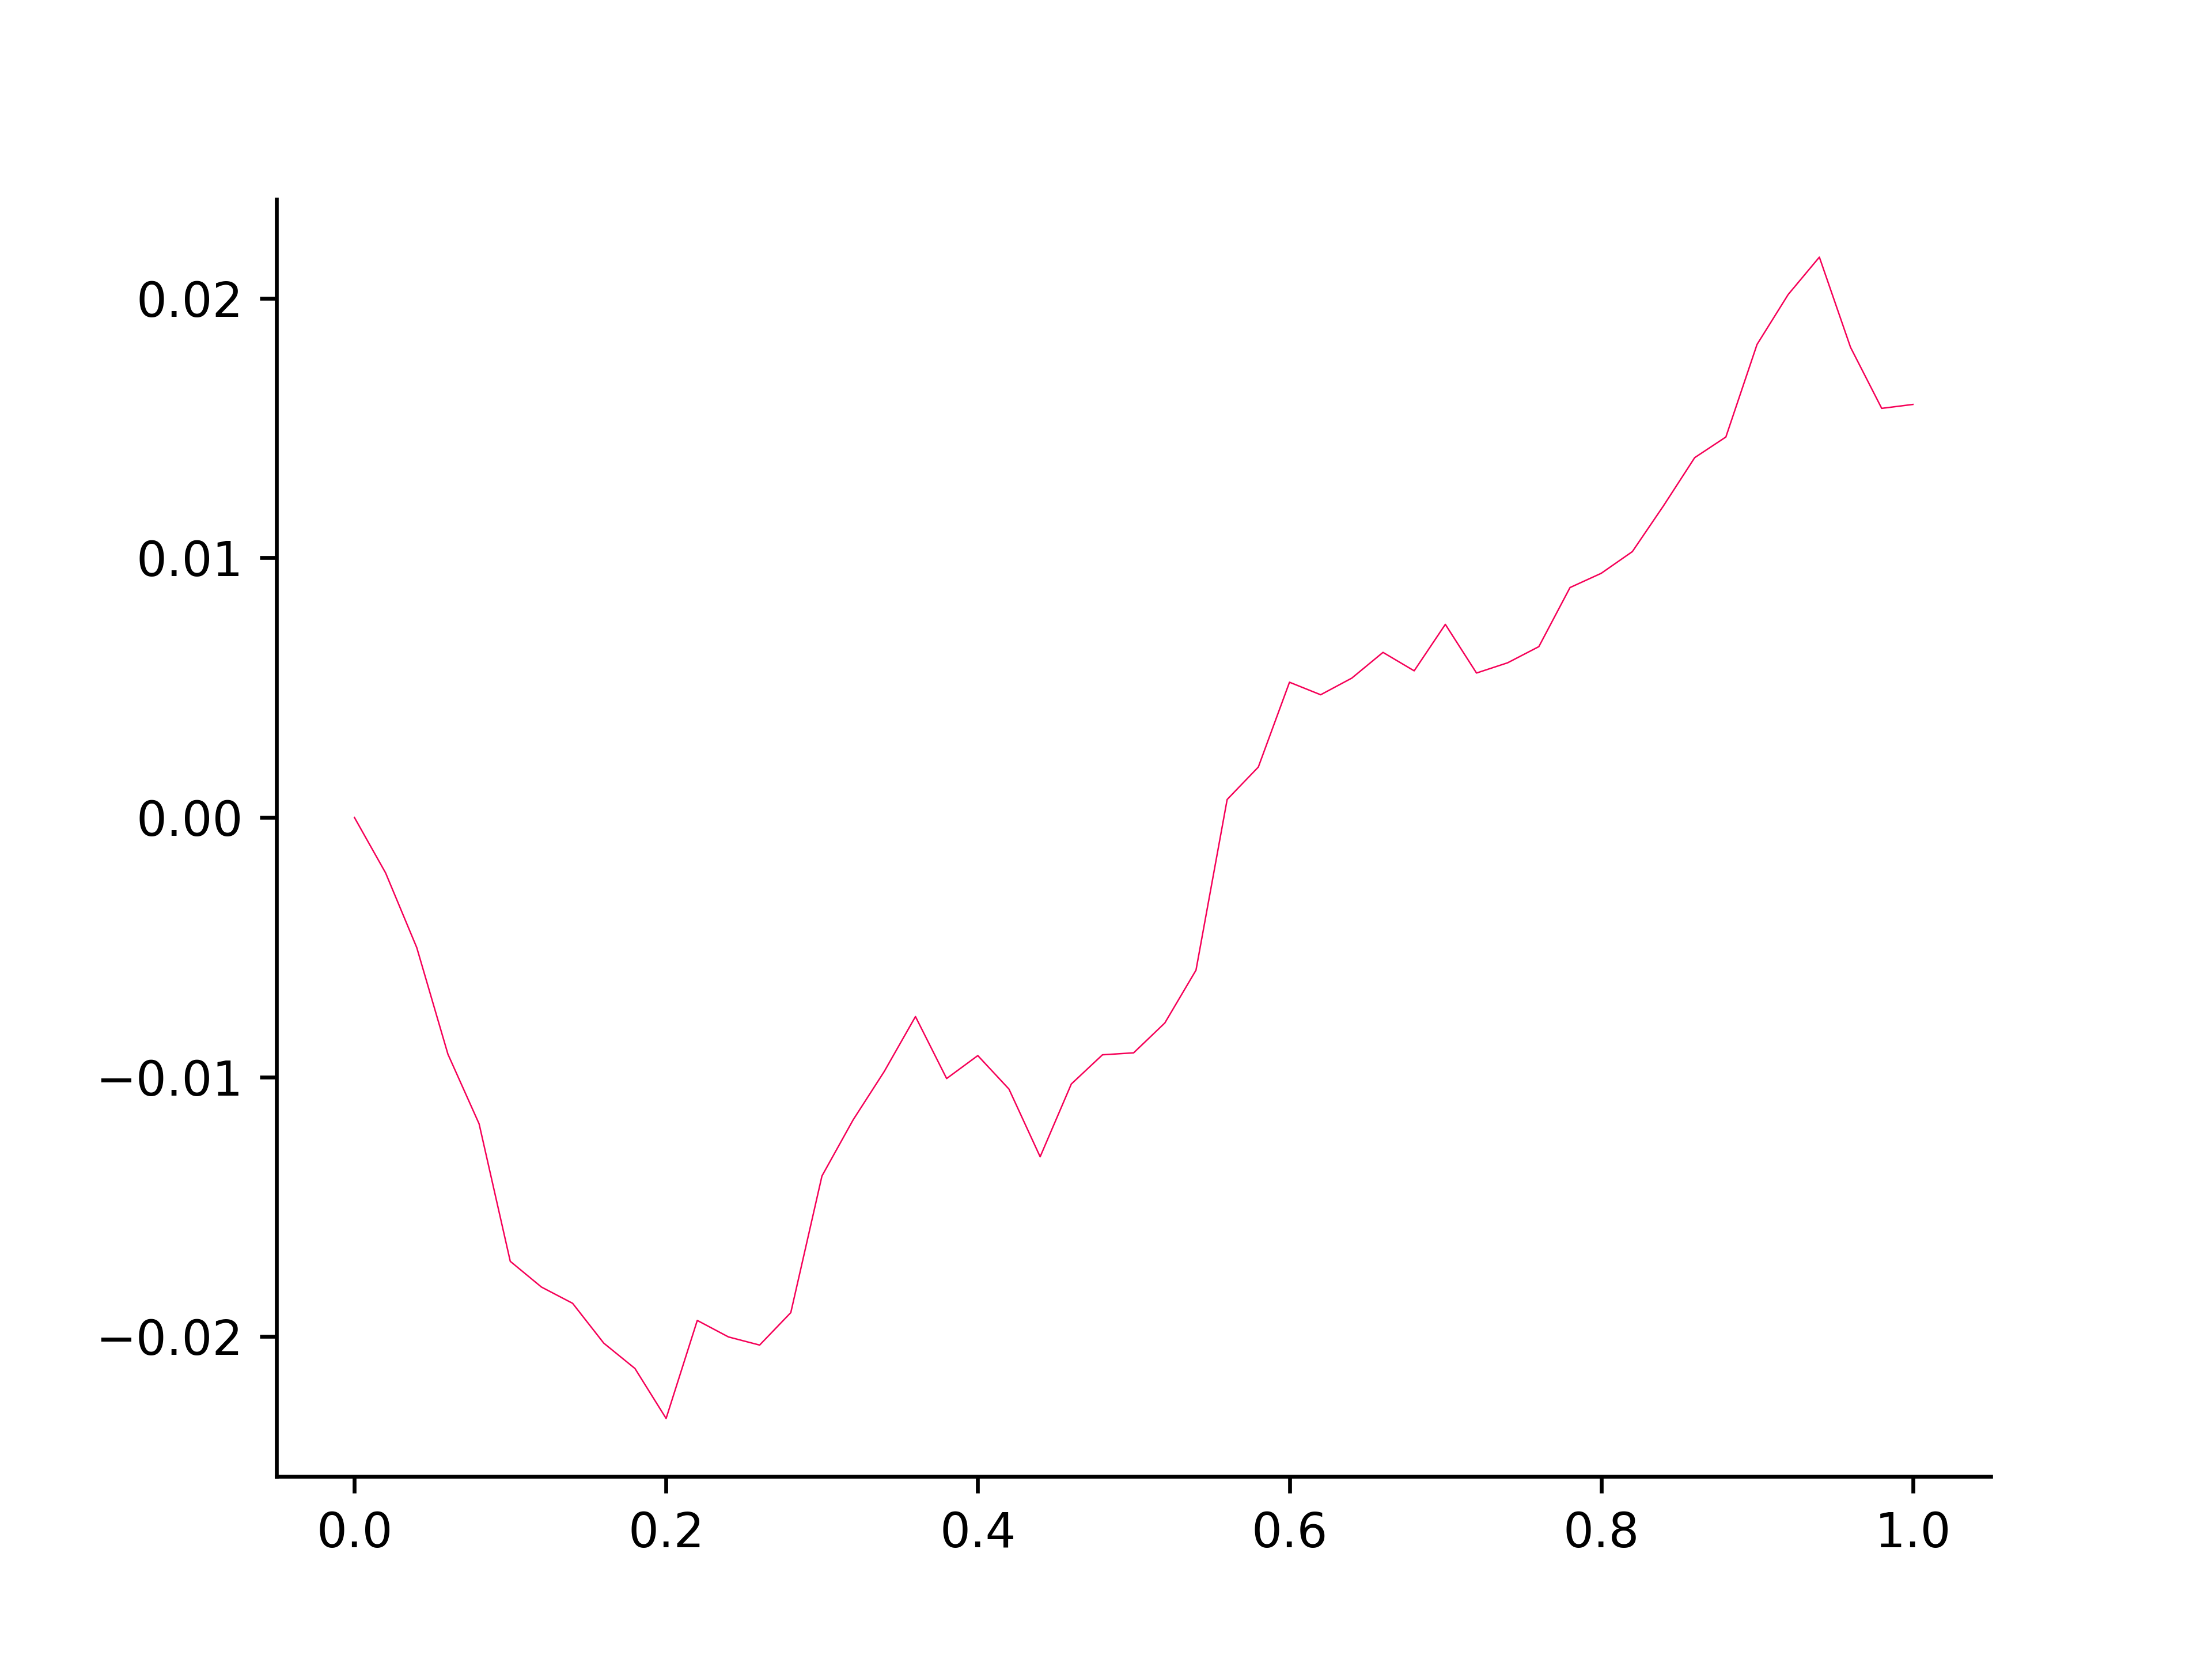
\includegraphics[scale=0.4]{mean-2-55.png}
		\caption{H=0.55}
		\endminipage\hfill
		\minipage{0.49\textwidth}
		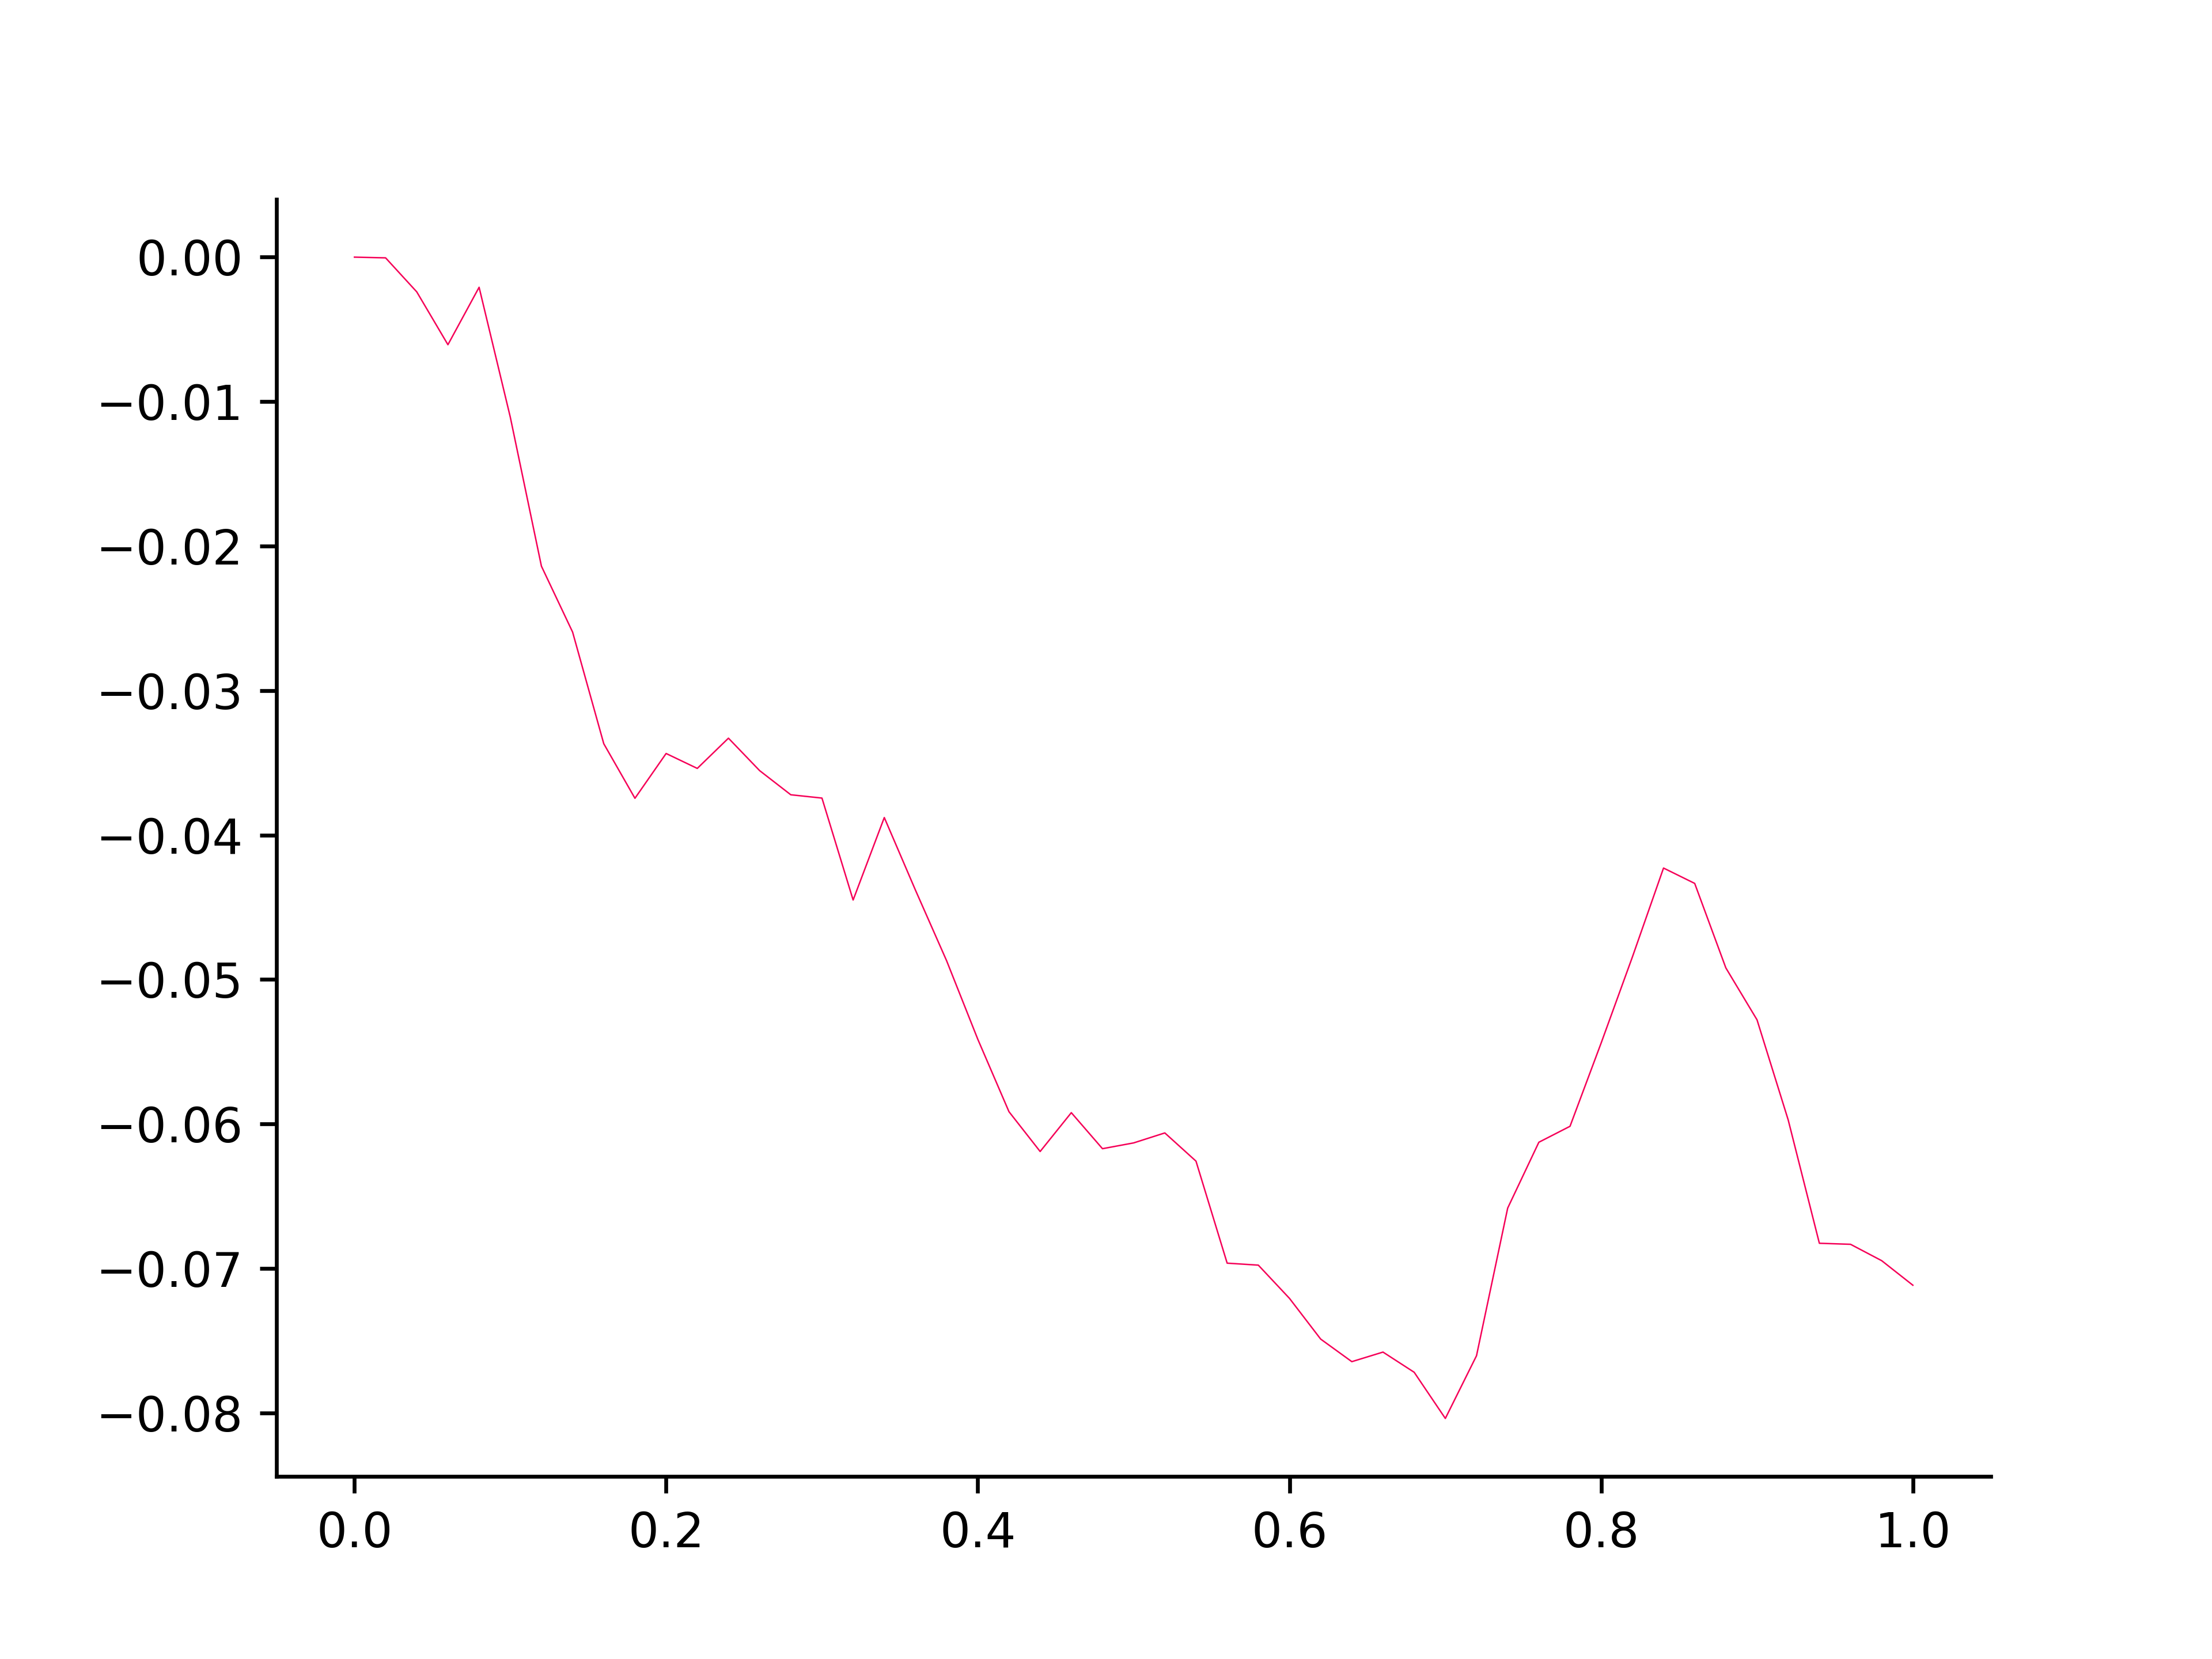
\includegraphics[scale=0.4]{mean-2-75.png}
		\caption{H=0.75}
		\endminipage\hfill
	\end{figure}
	
	\begin{figure}[H]
		\center
		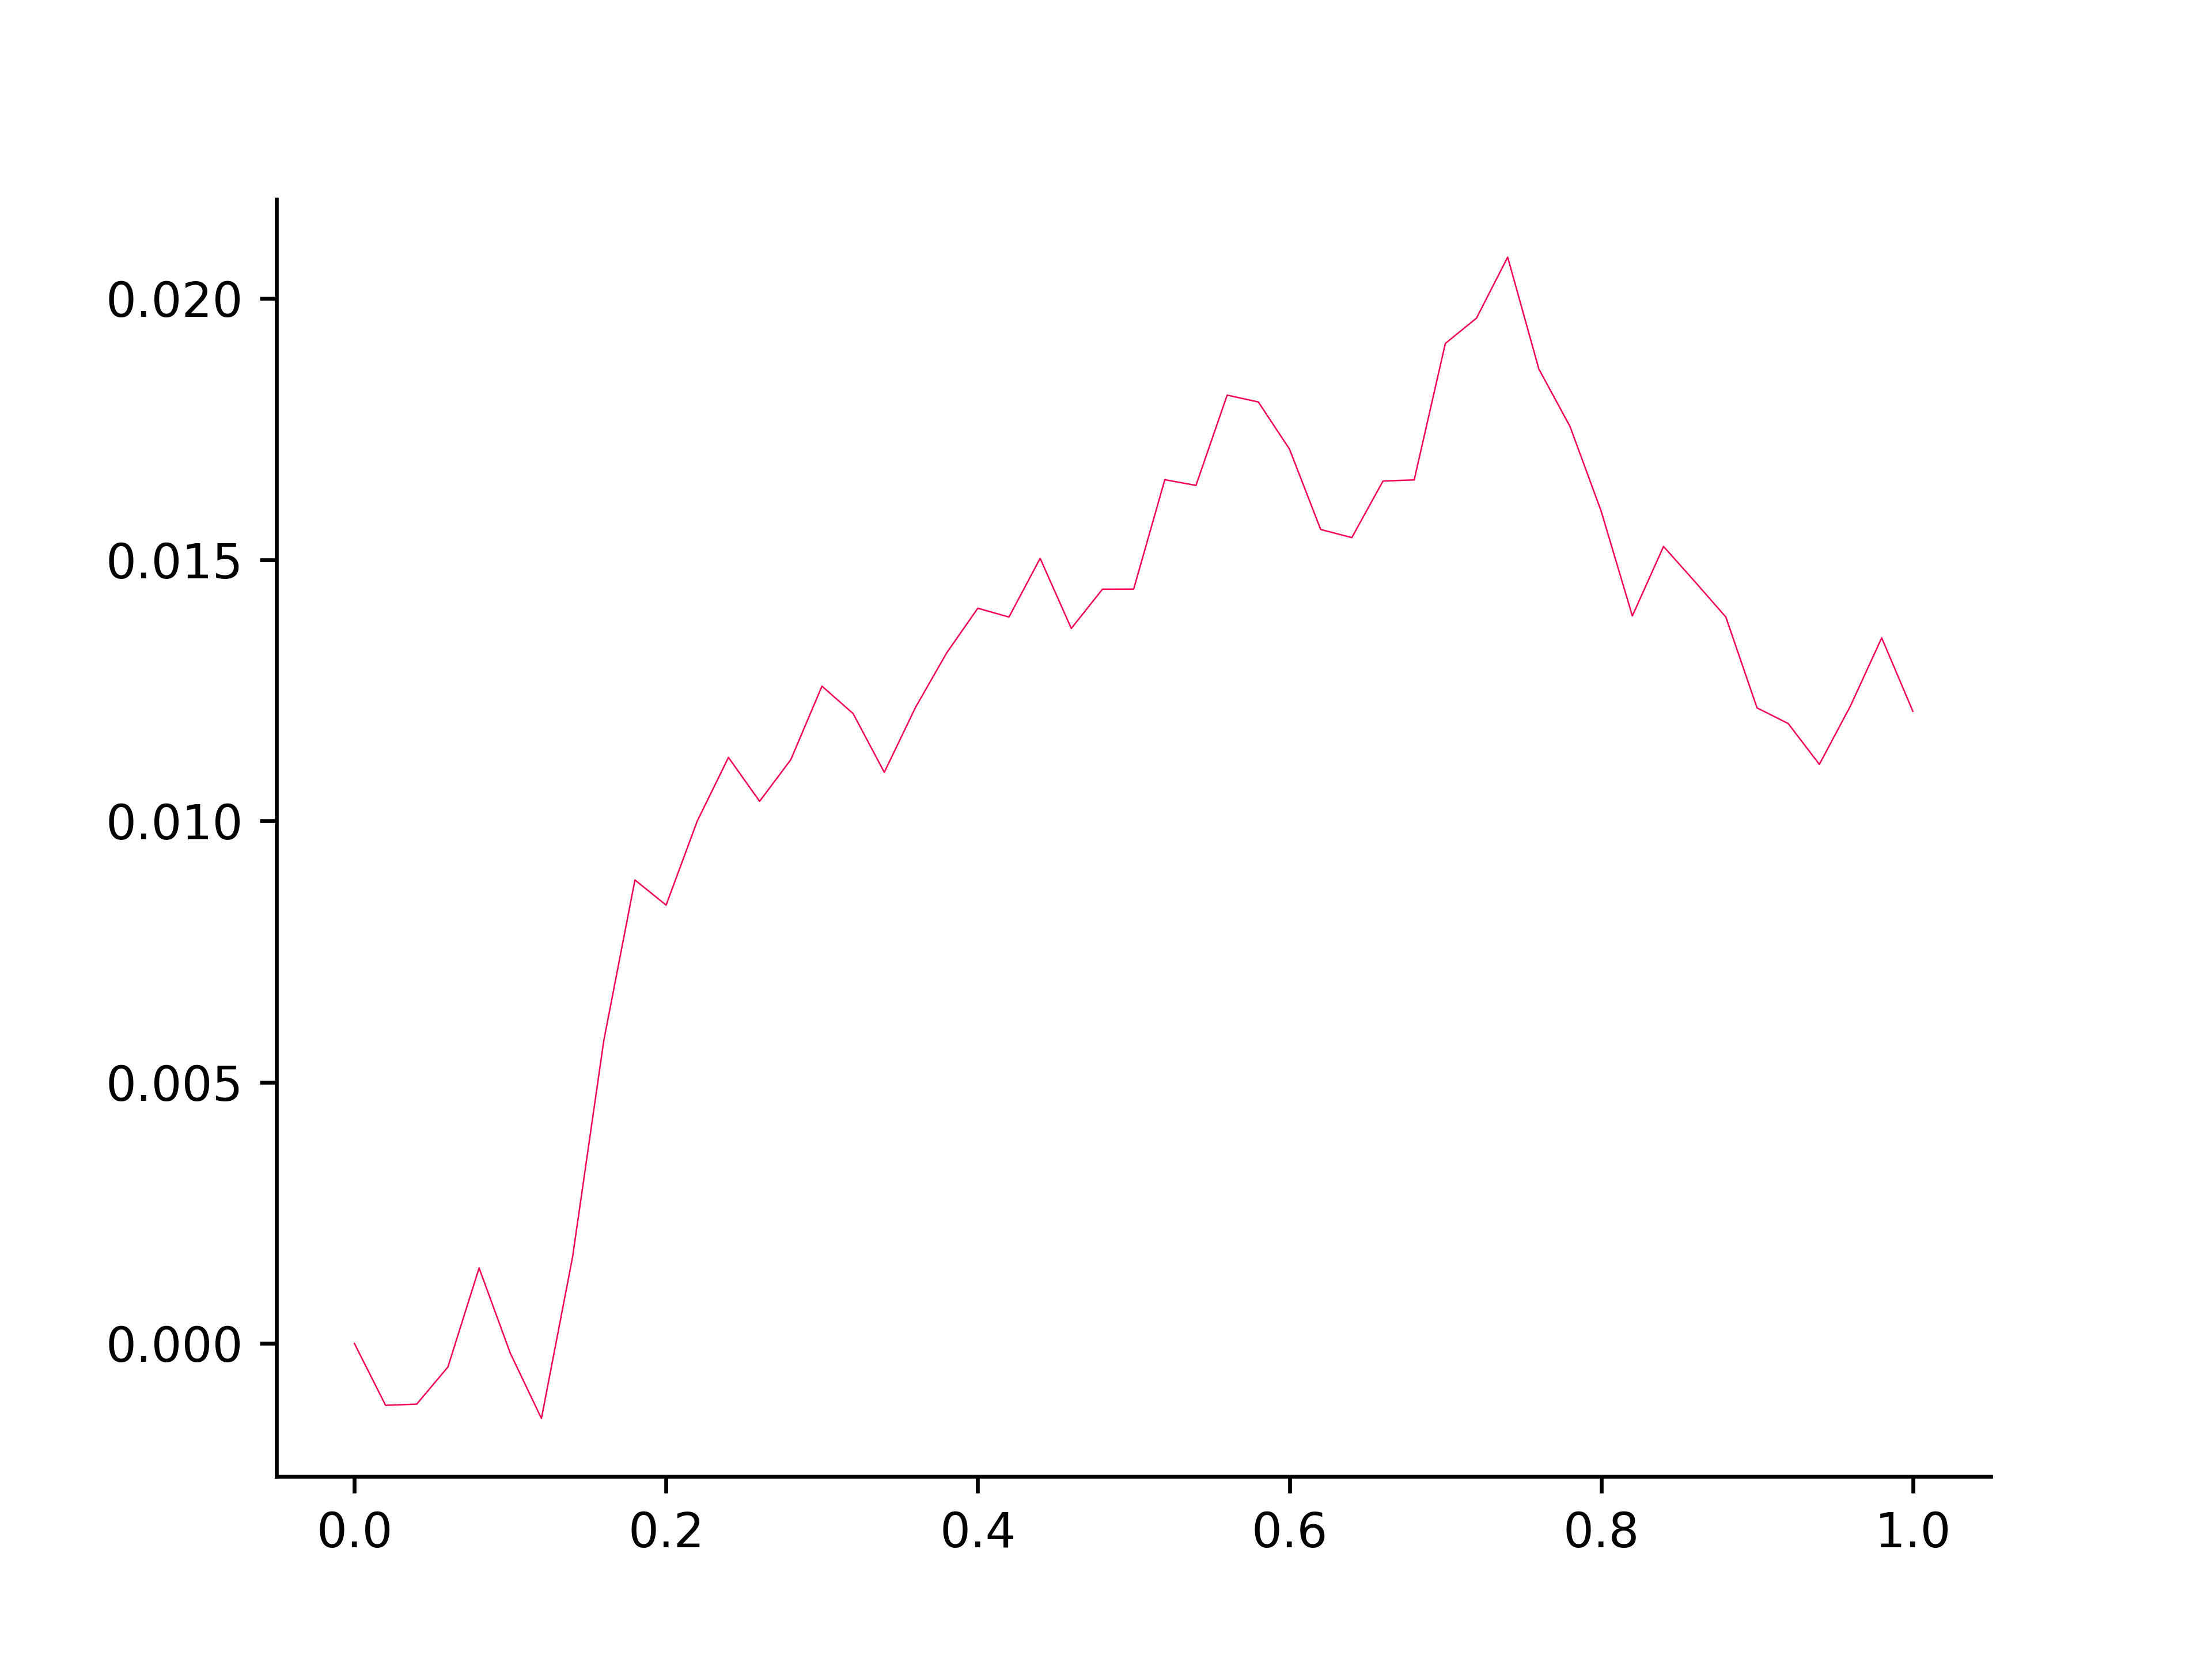
\includegraphics[scale=0.4]{mean-2-85.png}
		\caption{H=0.85}
	\end{figure}
	
	\section{Вывод}
	
	Из полученных результатов можно сделать вывод, что первый алгоритм позволяет моделировать дробное броуновское движение корректно. 
	
	Однако при выполнении второго алгоритма число участков моделирования случайно, а поэтому некоторые траектории сильно выделяются на общем фоне.
	\newpage
	\begin{thebibliography}	{99}
		\bibitem{Sam} G.Samorodnitsky, M.S.Taqqu,
		\textit{Stable non-Gaussian Random Processes}, Chapman and Hall, NY, 1994.
		
		\bibitem{Rusakov} Rusakov, O., Yakubovich, Y., Ласкин, М. Б., \textit{Self-similarity for information flows with a random load free on distribution: The long memory case}. In Proceedings - 2018 2nd European Conference on Electrical Engineering and Computer Science, EECS 2018 (pp. 183-189). [8910097]. 
		
		\bibitem{Devroye} Luc Devroye, \textit{Non-Unifrom Random Variate Generation}, 1986.
	\end{thebibliography}
\end{document}